\documentclass[12pt]{report}
\usepackage{graphicx} % Required for inserting images
\linespread{1.2}

\usepackage[dvipsnames]{xcolor}
\usepackage{tikz}
\usepackage[breakable]{tcolorbox}
\appto{\bibsetup}{\raggedright}

\tikzstyle{mybox} = [draw=Dandelion, fill=Dandelion!5, ultra thick, rectangle, rounded corners, inner sep=10pt, inner ysep=15pt, text width=0.90\textwidth, align=left] 
\tikzstyle{boxtitle} = [fill=Dandelion, text=Brown, ultra thick, rectangle, rounded corners, inner sep=10pt, inner ysep=8pt, text width=0.90\textwidth]

\newcommand{\BoxDef}[2]{%
\vspace*{10px}
\noindent

\begin{center}
\begin{tikzpicture}
    \node[mybox](box){\rule{0pt}{30pt}\ignorespaces#2\unskip};
    \node[boxtitle, anchor=north west] at (box.north west) {\textbf{#1}};
\end{tikzpicture}
\end{center}
}

\usepackage[]{hyperref}
\usepackage{amsmath}
\usepackage{amssymb}
\usepackage{bm}
\usepackage[top=2.5cm, bottom=2.5cm, left=3cm, right=3cm, centering]{geometry}
\usepackage{algorithm}
\usepackage{algpseudocode}
\usepackage{tabularx}
\usepackage{tabularray}

\begin{document}

\begin{titlepage}
\hrule
\vspace{15pt}
\begin{center}
    \Huge{\textbf{\Huge \textbf{Data Mining 2 23-24}} \\ Notes}\\
\end{center}
\vspace{15pt}
\hrule
\vfill
\hrule
\begin{center}
    \Large University of Pisa \\ M.Sc. in Data Science and Business Informatics
\end{center}
\end{titlepage}

\tableofcontents

\chapter{Rule Based Models}

A rule based classifier is a model that uses a \textbf{rule set} of ``if-then'' rules to classify instances. Each rule is expressed in the form:
\begin{equation*}
    r_i : (Cond_i) \xrightarrow{} y_i.
\end{equation*}
The left side contains a conjunction of attribute test conditions, and is called \textbf{antecedent} or \textbf{precondition}, while the right side represents the predicted class, and is called the \textbf{consequent}. Each condition is defined by a set of $k$ attribute-value pairs, such that:
\begin{equation*}
    Cond_i = (A_1 \ op \ v_1) \land (A_2 \ op \ v_2) \land \dots \land (A_k \ op \ v_k) \ ,
\end{equation*}
where $op$ is a comparison operator. Each attribute test is also known as a \textbf{conjunct}.

A rule $r$ \textbf{covers} an instance $x$ if the attributes of the instance satisfy the antecedent of the rule. Consider the following dataset:
\begin{table}[h]
    \centering
    \begin{tabular}{|c|c|c|c|}
    \hline
        Name & Can Fly & Gives Birth & Blood Type \\
    \hline
    \hline
        Bat & Y & Y & W \\
    \hline
        Owl & Y & N & W \\
    \hline
        Crocodile & N & N & C \\
    \hline
        Platypus & N & N & W \\
    \hline
    \end{tabular}
    \caption{Small example dataset.}
    \label{tab:small_dataset}
\end{table}
\\The rule $(Can Fly = Y) \land (Gives Birth = N) \xrightarrow{} Bird$ covers the instance ``Owl''.

The \textbf{coverage} of a rule is the fraction of records in the whole dataset that are covered by it. The \textbf{accuracy} (sometimes called \textbf{precision}) of a rule is the fraction of records in the dataset that satisfy the antecedent that also satisfy the consequent.
\BoxDef{Coverage and Accuracy}{
\begin{align*}
    &Coverage(r) = \dfrac{|A|}{|D|} \\\\
    &Accuracy(r) = \dfrac{|A \cap y|}{|A|}
\end{align*}
}

\section{How Rule-Based Models Work}

A rule based classifier classifies a test instance based on the rule triggered by the instance. Looking at the dataset pictured in Table \ref{tab:small_dataset}, assume we obtained the following rule set from a training set:
\begin{align*}
    &r_1 : (Can Fly = Y) \xrightarrow{} Bird \\
    &r_2 : (Gives Birth = Y) \land (Blood Type = W) \xrightarrow{} Mammal \\
    &r_3 : (Blood Type = C) \xrightarrow{} Reptile
\end{align*}
The instance Owl triggers the first rule, and is therefore classified as a $Bird$. The Bat triggers both the first and the second rule, which produce conflicting outcomes. None of the rules cover the example Platypus, so there's no immediate way to assign a class to this animal. The following section will explain how these issues can be solved.

\section{Properties of a Rule Set}

The rule set generated by the model can be characterized by the following two properties:
\BoxDef{Mutually Exclusive Rule Set}{
The rules in a rule set $R$ are mutually exclusive if no two rules in $R$ are triggered by the same instance; this property guarantees that each instance is covered by at most one rule in $R$.
}
\BoxDef{Exhaustive Rule Set}{
A rule set $R$ is exhaustive if each combination of attribute values is covered by at least one rule.
}
Unfortunately, many rule based classifiers do not have such properties. If the rule set is not exhaustive, a default rule with an empty antecedent can be added to classify all instances that are not covered by any other rule.

If the rule set is not mutually exclusive, the rules can be organized into an \textbf{ordered rule set} (also known as \textbf{decision list}).
\BoxDef{Ordered Rule Set}{
The rules in an ordered rule set $R$ are ranked in decreasing order of priority. 
}
The rank of the rule can be defined via either \textbf{rule-based ordering} (rules are ranked based on their quality, e.g., their accuracy) or \textbf{class-based ordering} (all rules that have the same consequent appear together). When a test instance is presented to the model, it is compared with the rules starting from the one at the top of the ranking, and the prediction will be the one appearing as the consequent of the highest ranking rule that covers the instance. If none of the rules are triggered, the default rule is reached, classifying the instance as the default class.

Another approach is to use a \textbf{voting scheme}, where, for each test instance, votes are accumulated for each class assigned to it by the rules it triggers. The prediction will correspond to the class with the highest number of votes, and votes may also be weighted depending on the rule that is producing it (for example, rules with lower accuracy will produce votes with lower weight).

The advantage of using an unordered rule set is that they're less susceptible to errors, since they are not biased by the chosen ordering. Model building is also less expensive, since the rules don't have to be sorted. On the other hand, classification can be more costly, since the same instance must be first compared to all the rules in the rule set before evaluating the votes.

\section{Building a Rule Set}

Rule extraction methods can be either:
\begin{itemize}
    \item \textbf{Direct}, if the rules are extracted from the data itself;
    \item \textbf{Indirect}, if the rules are extracted from some other model (e.g., Decision Trees).
\end{itemize}

\subsection{Direct Methods for Rule Extraction}

To illustrate how direct methods work, we'll consider a widely-used algorithm called \textbf{RIPPER} (Repeated Incremental Pruning to Produce Error Reduction). This algorithm scales almost linearly with the number of training examples, and is particularly suited for datasets with imbalanced class distributions. It also works well with noisy data, since it uses a validation set to prevent overfitting.

RIPPER uses the \textbf{sequential covering} algorithm to extract rules from data. This algorithm uses a greedy strategy to build rules, one class at a time. For binary problems, the majority class is chosen as the default, and the algorithm learns the rules to detect only the minority class. For multiclass problems, the classes are first ordered by prevalence in the dataset; then, starting from the least prevalent class $y_1$, all elements belonging to it are labeled as positive, while all the rest, belonging to $y_2, y_3, \dots y_c$, are labeled as negative. The sequential covering algorithm learns a set rules that discriminates between these positive and negative classes. Next, all instances in $y_2$ (the second least prevalent class) are labeled as positive, while all instances belonging to $y_3, y_4, \dots y_c$ are labeled as negative, and a new rule set is constructed. This process is repeated until only one class remains, $y_c$, which is designated as the default one.

\begin{algorithm}
\caption{Sequential covering algorithm.}
\begin{algorithmic}[1]
    \State $E$ = TR instances, $A$ = set of attribute-value pairs
    \State $Y_{\sigma} = \{y_1, y_2, \dots , y_k\}$
    \State $R = \{ \}$

    \For{each $y \in Y_{\sigma} - \{y_k\}$}
        \While{stopping cond is False}
            \State $r \xleftarrow{}$ Learn-One-Rule($E,A,y$)
            \State Remove TR instances from $E$ that are covered by $r$.
            \State $R \xleftarrow{} R \lor r$
        \EndWhile
    \EndFor
    \State Insert default rule: $R \xleftarrow{} R \lor (\{\} \xrightarrow{} y_k)$
\end{algorithmic}
\end{algorithm}

The algorithm always starts with an empty decision list, $R$, and extracts rules for each class following the ordering specified by their prevalence. The Learn-One-Rule function iteratively extracts all rules for the current class, and all training instances covered by each rule found is removed from $E$. The rule is then added to the bottom to the rule list, and the loop repeats until the specified stopping criterion is met.

\subsubsection{Rule Evaluation}

In the Learn-One-Rule function, the algorithm must search for an optimal rule by growing one in a greedy fashion. It starts with a rule with an empty antecedent, $r : \{ \} \xrightarrow{} +$. Then, new conjuncts are gradually added to the antecedent in order to improve the rule's accuracy.

RIPPER uses the \textbf{FOIL's First Order Inductive Learner) information gain} as the measure to choose which conjunctive to add to the rule's antecedent.

\BoxDef{FOIL's Information Gain}{
Given $p_0$ and $n_0$ the number of positive and negative examples covered by the original rule, and $p_1$ and $n_1$ the number of positive and negative examples covered by the new rule, the FOIL's information gain is defined as:
\begin{equation*}
    FOIL's \ inf. gain = p_1 \times \left( \log_2 \dfrac{p_1}{p_1 + n_1} - \log_2 \dfrac{p_0}{p_0 + n_0} \right)
\end{equation*}
}
RIPPER starts with a rule $r : A \xrightarrow{} +$. It then adds one conjunct, $B$, generating the rule $r : A \land B \xrightarrow{} +$, and the information gain is calculated for this addition. This step is repeated for different conjuncts, and the rule with the highest information gain is chosen to replace the original rule. The function stops once there's no additions that improve the information gain, so the rule covers only positive instances. Additionally, all instances covered by the rule are removed from the training set.

RIPPER also performs pruning of the rules to improve the generalization error based on their performance on a validation set. After generating a rule, the following metric is computed:
\begin{equation*}
    v = \dfrac{(p-n)}{(p+n)} \ ,
\end{equation*}
where $p$/$n$ are the number of positive/negative validation instances covered by that rule. If this measure improves after removing a conjunct, the latter is permanently pruned, and the measure is again evaluated for the next conjunct. The check follows the reverse order to the one established by the insertion of conjuncts during generation. Note that a pruned rule may cover both positive and negative examples of the training set; this means that the rule is less adapted to the training data, but performs better on unseen examples. 

The generation of rules is interrupted once a stopping condition is verified, such that the complexity of the model is high enough to generalize well, but not so high that it overfits the training data. Some common stopping conditions are evaluated based on the \textbf{Minimum Description Length} (\textbf{MDL}). The MDL measures the cost of a model as:
\begin{equation*}
    Cost(M, D) = Cost(D|M) + \alpha \times Cost(M) \ ,
\end{equation*}
where $M$ and $D$ are the model and the data, respectively, and $\alpha$ is a tuning hyperparameter (usually set to 0.5).  The first term of the addition encodes the misclassification error, while the second term uses node encoding (number of children) plus encoding of the splitting condition. The cost is evaluated in terms of how many bits are needed to encode the rule set: if the addition of a rule would increase the length of the set by at least $d$ bits, then RIPPER stops adding rules (by default, $d$ is 64 bits). This is a form of Pessimistic Error Estimate, since it evaluates the generalization error of the model as:
\begin{equation*}
    R(T) = R_{emp} + \Omega \times \dfrac{k}{l} \ ,
\end{equation*}
where $R_{emp}(T)$ is the training error, $\Omega$ is a trade-off hyperparameter that represents the cost of adding a new rule, $k$ is the size of the rule set, and $l$ is the number of training instances.

RIPPER also performs additional optimization steps to determine whether the rules in the set can be replaced by better alternatives. For each rule $r$, two new rules are considered as replacement:
\begin{itemize}
    \item A replacement rule $r^*$: a new rule is grown from scratch;
    \item A revised rule $r'$: conjuncts are added to the rule $r$ to extend it.
\end{itemize}
The rule set for $r$ is compared with the rule sets for $r^*$ and $r'$, choosing the rule that minimizes the MDL.

\subsection{Indirect Methods for Rule Extraction}

Indirect methods generate a rule set by using the output of some other model, typically an unpruned decision tree. In a decision tree, each path connecting the root to a leaf can be expressed as a classification rule, where each attribute test condition encountered on the path is a different conjunct of the antecedent, and the (majority) class in the leaf node is the consequent. This section will focus on the approach followed by the algorithm C4.5rules.

A rule is generated from each path in the tree. For each rule $r : A \xrightarrow{} y$ in the rule set, alternative rules $r' : A' \xleftarrow{} y$ are considered, where $A'$ is obtained by removing one of the conjuncts in $A$. The simplified rule with the lowest pessimistic error rate is retained as a replacement if the error rate is also lower than that of the original rule. Eventual duplicates of the new rule are eliminated from the rule set.

After generating the rule set, C4.5rules uses a class-based ordering to rearrange the rules, so that all rules predicting the same class appear close together in the same subset. The description length of each subset is calculated, and the classes are arranged in increasing order of their total description length. This way, the subset with the lowest description length is given priority over the others, since it is assumed to contain the best set of rules.

\section{Characteristics of Rule Based Models}

Rule based classifiers are very similar to decision trees, and have about the same expressiveness. Both models construct rectilinear decision boundaries in the input space, and assign a class to each partition. Rule based classifiers, however, can allow multiple rules to be triggered for the same instance, while in decision trees, each instance can only follow one specific path. Because of this, rule based models can approximate more complex functions.

Like decision trees, they can handle different types of attributes, both continuous and categorical, and can work for both binary and multiclass classification tasks. Additionally, rule based classifiers often produce models that are easier to interpret but have comparable performance to decision trees.

They can also handle redundant attributes, since if two or more highly correlated, only one of them is chosen to be added as a conjunct. Since irrelevant attributes will show poor information gain, rule based models will tend to avoid choosing them as conjuncts. Still, as seen for decision trees, if the problem is sufficiently complex, sometimes irrelevant attributes may be chosen over other more relevant ones that show poor information gain individually, but would be useful when interacting with others.

They cannot handle missing values in the test set, as the positioning of the rules in a rule set follows a specific ordering strategy, so if a test instance is covered by multiple rules they may produce conflicting outputs.

Since RIPPER uses a class-based ordering strategy, emphasizing classes with fewer instances, these models are very well suited for imbalanced class distributions. 
\chapter{Sequential Pattern Mining}

Sequential pattern mining is the discovery of subsequences that frequently appear in a sequential dataset, i.e., finding all the subsequences whose number of occurrences is greater or equal than a user-defined threshold ($minsup$). These frequent subsequences are also called \textbf{sequential patterns}. Unlike frequent itemset mining, sequences also contain spatio-temporal information that specifies when certain transactions happen. Common examples of sequential data may be the purchase history of customers in a supermarket, genome sequences, or web browsing history. 

\BoxDef{Sequence, element, event}{
    A sequence $s$ is an \textbf{ordered} list of elements $s = \langle e_1 e_2 \ldots e_n\rangle$. Each element (or ``transaction'') $e_j$ is an \textbf{ordered} list of one or more events (or ``items'') $e_j = \{ i_1, i_2, \ldots , i_m \}$. Each event is a literal.
}
Each event/item can occur only once in an element/transaction, but may occur multiple times in separate elements/transactions. Events in the same element appear according to lexicographical ordering. An example of a sequence is the following:
\begin{equation*}
    s = \langle \{1, 2, 3\} \{1\} \{1, 3\} \rangle \,.
\end{equation*}
The whole sequence is delimited by angle brackets $<,>$, and each element is delimited by curly brackets $\{,\}$.
This sequence contains three elements, three unique events, and a total of 6 events.
The \textbf{length} of a sequence ($|s|$) is the number of its elements. The \textbf{size} of the sequence is the total number of its events. A sequence of size $k$ is also known as a \textbf{$k$-sequence}.

\BoxDef{Subsequence}{
    A sequence $s = \langle s_1 s_2 \ldots s_n\rangle$ is a subsequence of a sequence $t = \langle t_1 t_2 \dots t_m\rangle$ if there exist integers $1 \leq i_1 < i_2 < \dots < i_k \leq n $ such that $s_1 \subseteq t_{i_1}, s_2 \subseteq t_{i_2}, \dots , s_n \subseteq t_{i_k}$.
}
If $s$ is a subsequence of $t$, then $s$ is \textbf{contained} in $t$.

Let \textit{D} be a dataset of one or more sequences, called data-sequences. Each data-sequence consists in a list of elements, ordered by increasing time. Each element is associated with a sequence-id, a timestamp, and a list of the events it contains. For simplicity, we will assume that elements occur at regular intervals and never overlap. For each pattern, we can calculate its \textbf{support} and \textbf{support count}, defined the same as they were defined for itemsets in association analysis.

\BoxDef{Support}{
    The support of a sequence $s$ is the fraction of data-sequences in a dataset $D$ that contain $s$.
}
\BoxDef{Support Count}{
    The support count of a sequence $s$ is the absolute number of data-sequences in a dataset $D$ that contain $s$.
}

For the purpose of sequential pattern mining, only a single valid occurrence of a sequence in a data-sequence is considered towards computing support, so even if a subsequence appears in $n$ different ways within the same data-sequence, its support count will only be increased by 1. We can now formally define sequential pattern mining as follows:
\BoxDef{Sequential Pattern Mining}{
    Given \textit{D} a dataset of data-sequences, and $minsup$ a user-defined minimum support threshold, the problem of mining sequential patterns
    is to find all sequences whose support $\geq minsup$; each such sequence is a \textbf{sequential pattern}, also called frequent sequence. 
}

Discovering all frequent sequences in a dataset is a computationally challenging task. The most basic algorithm that solves the problem uses a brute-force approach: generate all possible $k$-sequences for $k = 1,2,3 \ldots$, and compute support for every single one of them. The ones whose support is greater or equal than a $minsup$ threshold are declared frequent. However, the set of all possible candidate sequences is exponentially large and difficult to enumerate, even more than what was seen in association analysis. An event can appear multiple times in different elements within the same sequence, and elements arranged in different orders correspond to different sequences. This means that even when considering a relatively small set of events, the algorithm generates a large set of candidates; e.g., with only three unique events, the candidates generated for size $k = 2$ would be:
\begin{gather*}
    \langle\{i_1\} \{i_1\}\rangle, \langle\{i_1\} \{i_2\}\rangle, \langle\{i_1\} \{i_3\}\rangle, \langle\{i_1 i_2\}\rangle, \langle\{i_1 i_3\}\rangle \\ 
    \langle\{i_2\} \{i_1\}\rangle, \langle\{i_2\} \{i_2\}\rangle, \langle\{i_2\} \{i_3\}\rangle, \langle\{i_2 i_3\}\rangle \\
    \langle\{i_3\} \{i_1\}\rangle, \langle\{i_3\} \{i_2\}\rangle, \langle\{i_3\} \{i_3\}\rangle \,,
\end{gather*}
for a total of 12 candidates. As the number of items increases (it can easily be in the order of the hundreds, thousands, or more), the number of candidates would explode beyond what could be analyzed in appropriate time. Even if we were to generate candidates from input sequences, removing one item at a time and calculating support, we would still have a disproportionate amount of sequences to check.

One approach to solve the problem efficiently is to exploit the anti-monotonicity property of support and the Apriori property, already used for frequent itemset mining. As a reminder:
\BoxDef{Anti-monotone property}{
A measure $f$ possesses the anti-monotone property if for every itemset $X$ that is a proper subset of an itemset $Y$, it holds that $f(Y) \leq f(X)$.
}

\BoxDef{Apriori principle}{
    If a $k$-sequence is frequent, then all of its $k-1$-subsequences must also be frequent.
}

\section{Time Constraints}
\label{sec:tconstr}

Time constraints control how support is calculated by considering the time elapsed between elements of a sequence. For example, consider a dataset that represents market basket data: each product is an event, each individual purchase is an element, and each data-sequence is a set of purchases made by a customer within some interval of time (months or years). If we're interested in finding a correlation between certain products, we may want to limit the time passed between transactions: if a customer bought product $A$, and then bought product $B$ several months after, then the sequence $\langle \{A\} \{B\} \rangle$ is not significant for the purposes of our analysis. The time constraints are three: \textbf{maxspan}, \textbf{maxgap}, and \textbf{mingap}.

\BoxDef{maxspan}{
The $maxspan$ constraint specifies the maximum time passed between the first and last element of a sequence. If $t_{i,i+1}$ is the time passed between consecutive elements $i$ and $i+1$ of a data-sequence, then the following inequality must hold true:

\begin{equation*}
	\sum t_{i,i+1} \leq maxspan
\end{equation*}
}

\BoxDef{maxgap and mingap}{
The $maxgap$ and $mingap$ constraints specify the maximum time and minimum time passed between two consecutive elements of a sequence, respectively. If $t_{i,i+1}$ is the time passed between consecutive elements $i$ and $i+1$ of a data-sequence of length $n$, then the following inequality must hold true for $i = 1 \ldots (n-1)$:

\begin{equation*}
    mingap < t_{i,i+1} \leq maxgap
\end{equation*}
}
The $maxgap$ constraint violates the Apriori principle. A modification of this principle is used instead, which refers to \textbf{contiguous subsequences}: 

\BoxDef{Contiguous Subsequence}{
Given a sequence $s = \langle s_1s_2 \ldots s_n \rangle$, a sequence $t$ is a contiguous subsequence of $s$ if:

	\begin{itemize}
		\item $t$ is obtained by dropping an event from either $s_1$ or $s_n$;
		\item $t$ is obtained by dropping one event from any element $s_i$ that contains more than one event;
		\item $t$ is a contiguous subsequence of $w$, and $w$ is a contiguous subsequence of $s$.
	\end{itemize}
}
The Apriori principle can then be modified in the following way:
\BoxDef{Modified Apriori Principle}{
If a $k$-sequence is frequent, then all of its \textbf{contiguous} $k-1$-subsequences must also be frequent.
}

\section{Generalized Sequential Patterns Algorithm}

the Generalized Sequential Patterns (GSP) algorithm is an efficient algorithm that uses the anti-monotonicity of support to extract sequential patterns; it also supports time constraints. It is very similar to the Apriori algorithm, with the same exact basic structure. The pseudocode of the algorithm is presented in the next pseudocode block.

\begin{algorithm}
\caption{Generalized Sequential Patterns pseudocode.}
\begin{algorithmic}[1]
    \State $k=1$.
    \State $F_k = \{ i : i \in I \land s(i) >= minsup \}$ \# find all frequent 1-sequences
    \Repeat
        \State $k = k + 1$
        \State $C_k$ = \texttt{candidate-gen}
        \State $C_k$ = \texttt{candidate-prune}($C_k$, $F_{k-1}$)

        \For{all $t \in T$}
            \State $C_t$ = \texttt{subsequences}($C_k$, $t$)

            \For{all $c \in C_t$}
                \State $\sigma(c) = \sigma(c) + 1$
            \EndFor
        \EndFor

        \State $F_k = \{ c | c \in C_k \land s(c) \geq minsup \}$ \# find all frequent k-sequences
    \Until{$F_k = \emptyset$}
\end{algorithmic}
\end{algorithm}
The algorithm does a first pass over the dataset and computes support for all unique events, determining which 1-sequences (sequences with only a 1-event element) are frequent. The main loop of the algorithm has a candidate generation phase, a candidate pruning phase, and finally a support counting phase.

\subsection{Candidate generation}

This phase generates new candidate $k$-sequences by merging together the frequent $(k-1)$-sequences found in the previous iteration. There's two possible cases: 
\begin{itemize}
    \item For $k = 2$, all frequent 1-sequences are merged with each other (including with themselves). For each couple of events $i_1$ and $i_2$, the generated candidates will be: $\langle\{i_1\} \{i_2\}\rangle$, $\langle\{i_2\} \{i_1\}\rangle$, and $\langle\{i_1 i_2\}\rangle$, if $i_1 \neq i_2$; only $\langle\{i_1\} \{i_2\}\rangle$, if $i_1 = i_2$.

    \item For $k > 2$, two frequent $(k-1)$-sequences $s_1$ and $s_2$ are merged only if the subsequence obtained by dropping the first event from $s_1$ is the same as the one obtained by dropping the last event from $s_2$. Then, the candidate can be generated in two ways. 
    
    If the last element of $s_2$ has only one event, append that last element to $s_1$ and obtain the merged sequence.
    
    If the last element of $s_2$ has more than one event, append the last event of that last element to the last element of $s_1$ and obtain the merged sequence.
\end{itemize}
Note that a sequence can, in some cases, be merged with itself, as long as the conditions described above hold true. Also, this procedure is both complete and generates no duplicates.

\subsection{Candidate Pruning}

A $k$-candidate can be pruned if at least one of its $(k-1)$-subsequences is infrequent, since support shows anti-monotone property, and therefore its support can only be less-or-equal-than any of its subsequences. Pruning is done by dropping one event at a time from the $k$-candidate, and checking if the resulting $(k-1)$-sequence is contained in the frequent ones found in the previous iteration. If any of them are not frequent, the candidate can be discarded.

\subsection{Support Counting}

After the candidate set is pruned, the algorithm iterates over the data-sequences, and for each of them finds which $k$-candidates it contains, increasing their support count accordingly. At the end, all $k$-candidates whose support is less than $minsup$ are discarded, while the rest form the set of frequent $k$-sequences.

\section{Generalized Sequential Patterns and Time Constraints}

Introducing the $mingap$, $maxgap$, and $maxspan$ time constraints requires the support counting and candidate pruning procedures to be modified. Support counting must now consider the time gap between consecutive elements (for the $mingap$ and $maxgap$ constraints) and the overall span of the sequence (for the $maxspan$ constraint) when determining if a candidate is contained in a sequence. This means that the procedure can't simply determine the first occurrence of a candidate within a data-sequence, but must keep searching for an occurrence that satisfies all three constraints at once, such that $mingap < t_{i,i+1} \leq maxgap$, and $\sum t_{i,i+1} \leq maxspan$, where $t_{i,i+1}$ is the gap between consecutive elements in a data-sequence.

As for candidate pruning, the Apriori principle and anti-monotonicity of support no longer hold true because of the $maxgap$ constraint. If a candidate $c$ is being pruned, and all of its subsequences are checked, some of them may be infrequent, even though the candidate is actually a frequent sequence.

For example, let sequence $s = \langle \{1, 2\} \{2\} \{3\} \{4\} \rangle$ be a data-sequence, and sequence $c = \langle \{1\} \{2\} \{4\} \rangle$ a candidate sequence. If $maxgap = 2$, then $c$ is contained in $s$, but the subsequence $c' = \langle \{1\} \{4\} \rangle$ is not, because the gap between $\{1\}$ and $\{4\}$ is $3$.

Therefore, the procedure must check all of a candidate's contiguous subsequences, removing one event at a time only from the elements that contain two events or more. If at least one of the contiguous subsequences of a candidate is infrequent, the candidate can be pruned. This new pruning strategy ensures that no candidate frequent sequences are accidentally discarded, since it skips all the elements that, when removed, could produce a sequence that contains a gap between consecutive elements that violates the $maxgap$ constraint. However, this strategy inevitably decreases the effect that pruning has on the overall execution.
\chapter{Transactional Clustering}

Clustering is a task whose objective is to find grouping of objects of a dataset into sets, called clusters, where each member of a cluster is more similar to all other elements in the same cluster than it is to elements in different clusters. For numerical data, proximity between objects is measured using distances, typically Euclidean or Manhattan, since records with numerical attributes only can be interpreted as points in an $n$ dimensional space. However, these measures are not appropriate to carry clustering tasks on categorical attributes, which are used to represent transactional data. The biggest issue is that the way two transactions are deemed ``near'' each other does not correspond to geometrical proximity.

This issue can be illustrated with a simple example. Assume we have 4 transactions:
\begin{align*}
    &T1 = \{1,2,3,4\} \\
    &T2 = \{1,2,4\} \\
    &T3 = \{3\} \\
    &T4 = \{4\}
\end{align*}
Usually, transactional data can be represented with a set of boolean attributes, one for each item, where a value of ``1'' indicates the presence of the corresponding item, while a ``0'' indicates its' absence. In this case, the dataset will be represented as:
\begin{align*}
    &P1 = \{1,1,1,1\} \\
    &P2 = \{1,1,0,1\} \\
    &P3 = \{0,0,1,0\} \\
    &P4 = \{0,0,0,1\} \\
\end{align*}
If Euclidean distance were used to calculate how far or close there transactions are to each other, we would find out that the distance between transactions 3 and 4 is:
\begin{equation*}
    d(P3, P4) = \sqrt{(0)^2 + (0)^2 + (1)^2 + (-1)^2} = \sqrt{2}    
\end{equation*}
However, the two transactions don't share any item, making them completely different.

This chapter will present four different algorithms that can cluster categorical data, each of which define proximity between transactions in different ways.

\section{K-Modes}

K-modes is similar to K-means, but can be used for categorical attributes. It starts by randomly choosing $k$ data points at random to elect to representative points. The algorithm then enters a loop, in which it assigns all points to the closest mode, recomputes the mode of each cluster, and repeats the past two steps until no object changes assignment between two successive iterations (or until some stopping criterion is verified).

The distance between two records is calculated as the number of mismatches between their attributes:
\begin{gather*}
    d(X,Y) = \sum_i \delta(x_i, y_i) \\
    \delta(x,y) = \begin{cases}
        0 & (x = y) \\
        1 & else
    \end{cases}
\end{gather*}
The representative object of a cluster is calculated as the mode of the objects in the same cluster.

This algorithm minimizes the function:
\begin{equation*}
    P(W,Q) = \sum_{i}^k \sum_{j}^n w_{i,j} d(x_i, Q_i) \,,
\end{equation*}
where $w_{i,j}$ is 1 if object $i$ belongs to cluster $j$, 0 otherwise, and $Q$ is the set of the modes of each cluster.

\section{ROCK (RObust Clustering using linK)}

ROCK is a hierarchical algorithm that uses \textbf{neighborhoods} and \textbf{links to clusters} to define closeness between two transactions. Neighborhoods are calculated locally, while links are calculated globally. The algorithm can be split into three main parts:
\begin{enumerate}
    \item \textbf{A random sample is drawn from the dataset}. A sample of points is uniformly extracted, using it to form clusters instead of the entire data. This ensures the algorithm can be used even on very large dataset while still producing an accurate enough clustering.

    \item \textbf{An agglomerative hierarchical clustering algorithm is performed on the sample}. ROCK follows the same steps as other hierarchical agglomerative algorithms: it starts by assigning each point to a singleton cluster, then computes the similarity measure for all pairs of clusters, and merges the two ``closest'' objects. These steps repeat until some stopping condition is met (usually, until $k$ clusters are formed).

    Two objects $A$ and $B$ are \textbf{neighbors} if their similarity is greater or equal than some hyperparameter threshold $\theta$, chosen between 0 and 1:
    \begin{equation*}
        A \in N_B \land B \in N_A \iff sim(A,B) \geq \theta \,,
    \end{equation*}
    where similarity is calculated with Jaccard's coefficient (the ratio of the number of matching items between the objects and the total number of distinct items between the two):
    \begin{equation*}
        sim(A,B) = \dfrac{|A \cap B|}{|A \cup B|}
    \end{equation*}
    A point is also considered a neighbor of itself.

    A \textbf{link} is calculated as the number of common neighbors between two objects:
    \begin{equation*}
        link(A,B) = |N_A \cap N_B|
    \end{equation*}
    Higher values of link means that there's a higher probability that the two objects belong to the same group (since they share neighbors). 
    
    \item \textbf{The entire dataset is labeled by assigning each object to a cluster}. A random sample is selected from each cluster, and each point $p$ in the original dataset is assigned to the cluster $i$ such that $p$ has the maximum number of neighbors in the corresponding sample.
\end{enumerate}
The best clusters are the ones that maximize the criterion function of the algorithm:
\begin{align*}
    &E_l = \sum_{i=1}^k n_i \sum_{p_q,p_r \in C_i} \dfrac{link(p_q, p_r)}{n_i^{1 + 2 f(\theta)}} \,, \\
    & f(\theta) = \dfrac{1-\theta}{1+\theta}
\end{align*}
where $n_i$ is the size of cluster $C_i$. This function penalizes clusters that present very few links compared to the expected number of links in the entire cluster, so that we avoid that objects with a low number of links are assigned to the same cluster. At each merging step of the algorithm, the two clusters that are merged are the ones that maximize the goodness measure:
\begin{equation*}
    g(C_i, C_j) = \dfrac{link(C_i, C_j)}{(n_i + n_j)^{1+2f(\theta)} - n_i^{1+2f(\theta)} - n_j^{1+2f(\theta)}} \,,
\end{equation*}
where the numerator is the number of cross-links between the two clusters, and the denominator is the expected number of them.

\section{CLOPE (Clustering with sLOPE)}

CLOPE is a clustering algorithm that is efficient for high dimensional data. It uses an exclusively global criterion function that tries to increase the intra-cluster overlap of transactions. This is done by increasing the height-to-width ratio of the cluster histogram. It is especially suitable for big datasets with a high number of unique items, since it uses an array representation of the data instead of binary.

For each cluster, the width is calculated as the number of distinct items, while the height is calculated as the ratio between the total number of (non unique) items and the width. In the example below, the cluster has a width of 5 and a height of 2.4.
\begin{figure}[h]
    \centering
    \begin{minipage}{0.49\textwidth}
    \centering
    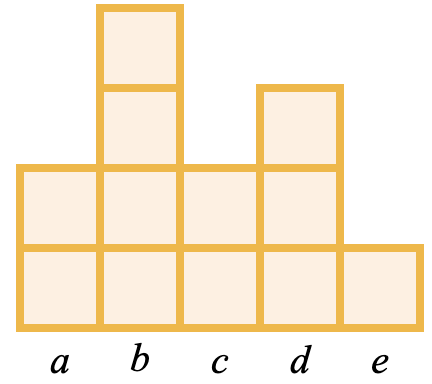
\includegraphics[width=0.5\linewidth]{img/CLOPE_cluster.png}
    \begin{equation*}
        C_i = \{abcd, bcd, ab, bde\}
    \end{equation*}
    \end{minipage}
\hfill
    \begin{minipage}{0.49\textwidth}
        \begin{gather*}
            W(C_i) = 5 \\
            S(C_i) = 12 \\
            H(C_i) = \dfrac{12}{5} = 2.4
        \end{gather*}
    \end{minipage}
\end{figure} \\
Higher ratios of height/width mean higher item overlapping.

The goodness of a clustering is calculated as the \textbf{gradient} of each cluster:
\begin{equation*}
    Profit_r(C) = \dfrac{\sum_{i=1}^k \dfrac{S(C_i)}{W(C_i)^r} \times |C_i|}{\sum_{i=1}^k |C_i|}
\end{equation*}
The hyperparameter $r$ is called \textbf{repulsion}; for higher values of $r$, transactions within the same cluster must share a large portion of items, while for lower values transactions may share a lower amount of items, which can be useful for sparse databases.

The algorithm has two phases: first, each transaction is added to a new cluster or to an existing one such that the profit is maximized. Then, for each transaction, it is checked whether moving it to a different cluster improves profit, repeating this step until all transactions remain in the same cluster (no moves will improve the profit).

\section{TX-Means}

TX-Means is a parameter-free transactional clustering algorithm, and is useful to partition data obtained from a massive amount of different datasets. It finds a representative transaction for each cluster, which summarizes the pattern presented by the elements of that cluster. Like X-Means, it starts out with a cluster that contains all the objects in the dataset, and chooses how to recursively split it into subpartitions by using the Bayesian Information Criterion.
\begin{algorithm}
\caption{TX-Means pseudocode.}
\begin{algorithmic}[1]
    \State $r$ = \texttt{getRepr}($B$) \# get representative basket of entire set of baskets
    \State $r$ is added to queue $Q$

    \While{$Q \neq \emptyset$}
        \State $C, r$ are extracted from $Q$
        \State Common items are removed from $C$ and $r$
        \State $C1,C2,r1,r2$ = \texttt{bisectBasket}($C$)
        \If{$BIC(C1,C2,r1,r2) > BIC(C,r)$}
            \State Add $C1,C2,r1,r2$ to $Q$
        \Else
            \State Add $C, r$ to result 
        \EndIf
    \EndWhile

    \State Return result
\end{algorithmic}
\end{algorithm} \\
The algorithm starts by finding a representative for all objects in the dataset, then enters a loop in which each cluster currently in the queue is split. Each split is either accepted, reinserting the new subpartitions in the queue, or rejected, adding the parent cluster to the result, depending on whether it produces an improvement in the BIC score. Below is the pseudocode for the functions \texttt{getRepr()} and \texttt{bisectBasket()}.

\begin{algorithm}[H]
\caption{\texttt{getRepr} pseudocode.}
\begin{algorithmic}[1]
    \State $I$ = set of items not shared among all baskets in $B$
    \State $r$ = set of items in common to all baskets in $B$
    \State Calculate frequencies of items in $I$
    \State $i = 0$, $d_0 = \inf$
    \While{$I \neq \emptyset$}
        \State $i = i + 1$
        \State Add the items in $I$ with maximum frequency to $r$
        \State Calculate the distance $d_i$ between $r$ and the baskets in $B$ via Jaccard coefficient
        \If{$d_i \geq d_{i-1}$}
            \State Return $r$
        \Else
            \State Remove from $I$ items with maximum frequency
        \EndIf
    \EndWhile 
    \State Return $r$
\end{algorithmic}

\end{algorithm}
\begin{algorithm}
\caption{\texttt{bisectBasket} pseudocode.}
\begin{algorithmic}[1]
    \State $SSE = \inf$
    \State Select two random baskets $r1,r2$
    \While{True}
        \State $C1,C2$ = clusters obtained by assigning baskets to either $r1$ or $r2$
        \State $r1_{new}$ = \texttt{getRepr}($C1$)
        \State $r2_{new}$ = \texttt{getRepr}($C2$)
        \State $SSE_{new} = SSE(C1,C2,r1_{new},r2_{new})$
        \If{$SSE_{new} \geq SSE$}
            \State Return $C1,C2,r1,r2$
        \EndIf
        \State $r1 = r1_{new}$
        \State $r2 = r2_{new}$
    \EndWhile
\end{algorithmic}
\end{algorithm}
TX-Means is also scalable thanks to the following sampling strategy. A random subset of transactions is chosen from the dataset, and TX-Means is run on that subset, returning a set of clusters and their respective representative transactions. Then, all the remaining transactions in the dataset are assigned to the clusters using a nearest neighbor approach with respect to the representatives found by the algorithm.
\chapter{Time Series}

A \textbf{time series} is a collection of observations made sequentially in time, usually at constant time intervals. They can be constructed out of measurements of many different phenomenons, such as annual rainfall levels, earthquakes, fMRI data, quarterly earnings, audio/video data, and so on. Time series can analyzed through clustering, classification, motif discovery, rule discovery, forecasting, and trend/seasonality analysis. The key issues that arise when working with time series are:
\begin{itemize}
    \item \textbf{The amount of data to work with can be incredibly large}: for datasets with several different sources and short intervals of time between measurements, the size can be very high.

    \item \textbf{Similarity is not easy to estimate}: since series are complex objects with several values each, defining how two series can be considered similar is not as easy as it can be for numerical data.

    \item \textbf{Different data formats}: different series in the same dataset may be represented using a different scale or format; e.g., atmospheric temperatures recorded in both $^{\circ}C$ and $^{\circ}F$.

    \item \textbf{Different sampling rates}: while usually it is assumed that series are recorded all with the same rate, in many real life cases this may not be true. Different series may have different lengths and different time intervals.

    \item \textbf{Noise, missing values, and other defects}: as with other types of data, time series can also present noisy information or missing values.
\end{itemize}
The following sections will explain how some of these issues can be dealt with.

\section{Similarity Between Time Series}

\subsection{Structural-based Similarities}

Especially when analyzing long time series, similarity is calculated on a structural level. This means that global features are extracted from the time series, creating a feature vector, and measuring similarity looking at those features. Some examples are the mean and variance, maximum/minimum, skewness, mean and variance of the $1^{st}$ derivative, and so on.

A measure used to calculate structural dissimilarity is \textbf{compression based dissimilarity}, which is calculated as:
\begin{equation*}
    d(x,y) = \textit{CDM}(x,y) = \dfrac{C(x,y)}{C(x) + C(y)} \,,
\end{equation*}
where $C$ is a compression algorithm. The numerator is the compression of the concatenation of the two series, while the denominator is the sum of the compressions of the series done singularly: the Compression Dissimilarity Measure equal to 1 if the two series are unrelated, otherwise it is less than one. The smaller its value, the closer the series are to each other. CDM is never zero.

\subsection{Shape-based Similarities}

Shape-based similarities can be calculated using distance measures. Recall that distances have the following properties:
\begin{align*}
    &d(a,b) \geq 0, d(a,b) = 0 \iff a = b \ (\text{Positivity}) \\
    &d(a,b) = d(b,a) \ (\text{Symmetry}) \\
    &d(a,c) \leq d(a,b) + d(b,c) (\text{Triangle Inequality})
\end{align*}
One way to calculate shape-based dissimilarity is using Euclidean distance. Given two time series (with the same exact number of points/measurements), the Euclidean distance is calculated as if the series were points in an Euclidean space. However, this distance is very sensitive to distortions in the data, which should be removed in a preprocessing phase.\\
The most common distortions are:
\begin{itemize}
    \item \textbf{Offset translation}: the series have different offsets on the y axis. Calculating the distance without addressing this problem would return a value that is drastically larger than the actual shape distance. This can be corrected by subtracting each series with its own mean value.
    \begin{figure}[ht]
        \centering
        \begin{minipage}{0.40\textwidth}
         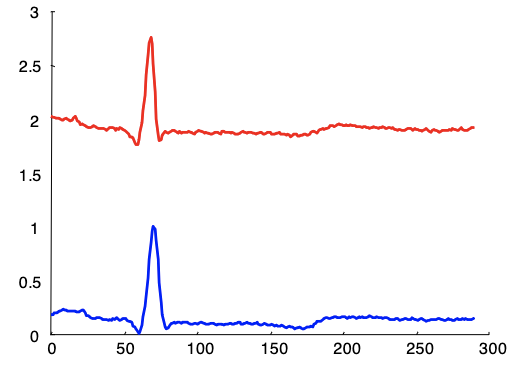
\includegraphics[width=1.0\linewidth]{img/offset_trans_1.png}
        \end{minipage}
        \hfill
        \begin{minipage}{0.40\textwidth}
            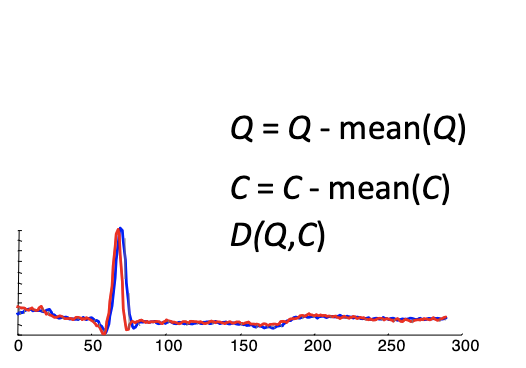
\includegraphics[width=1.0\linewidth]{img/offset_trans_2.png}
        \end{minipage}
        \label{fig:offset-trans}
        \caption{Offset translation transformation.}
    \end{figure}

    \item \textbf{Amplitude scaling}: the series have the same shape, but are scaled differently on the y axis. This is corrected by applying Z-score normalization to the values of the series (subtracting the mean and dividing by the standard deviation).
    \begin{figure}[ht]
        \centering
        \begin{minipage}{0.40\textwidth}
            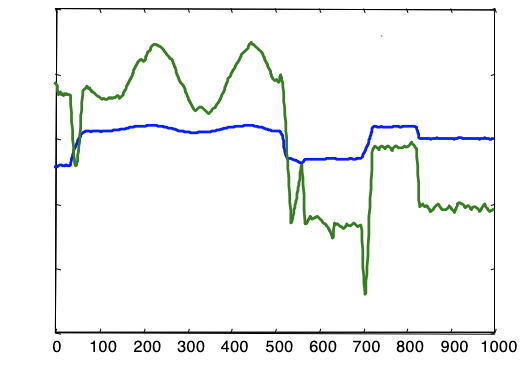
\includegraphics[width=1.0\linewidth]{img/ampli_scaling_1.png}
        \end{minipage}
        \hfill
        \begin{minipage}{0.40\textwidth}
            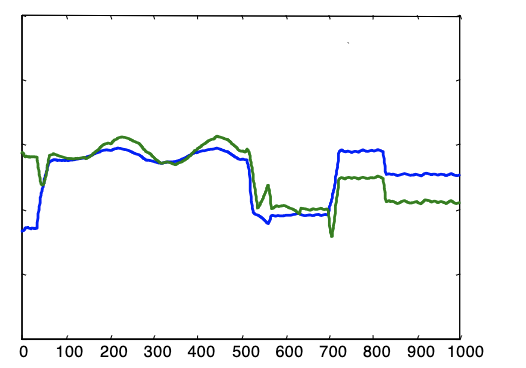
\includegraphics[width=1.0\linewidth]{img/ampli_scaling_2.png}
        \end{minipage}
        \caption{Amplitude scaling transformation.}
        \label{fig:ampli-scaling}
    \end{figure}

    \item \textbf{Linear trend}: series can follow upwards or downwards linear trends, which means that as they progress they increase or decrease in level. This can be corrected by finding the best fitting line to a time series, and subtracting it from the time series itself.
    \begin{figure}[ht]
        \centering
        \begin{minipage}{0.40\textwidth}
            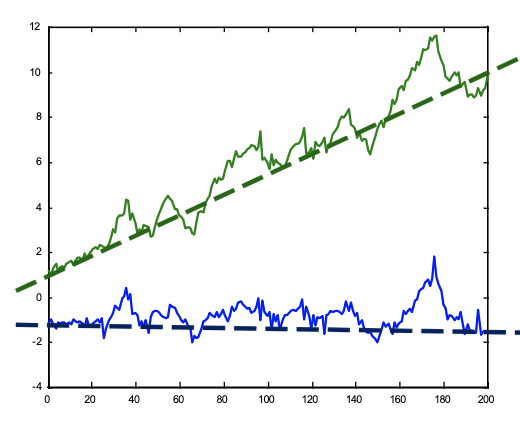
\includegraphics[width=1\linewidth]{img/lin_trend_1.png}
        \end{minipage}
        \hfill
        \begin{minipage}{0.40\textwidth}
            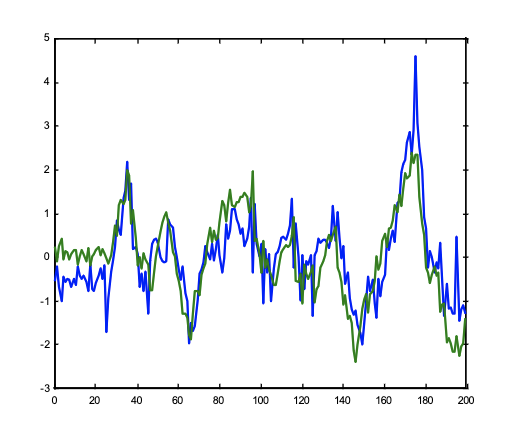
\includegraphics[width=1\linewidth]{img/lin_trend_2.png}
        \end{minipage}
        \caption{Linear trend transformation.}
        \label{fig:lin-trend}
    \end{figure}

    \item \textbf{Noise}: noise is the presence of random error in the series. To remove noise, each data point can be replaced with the average value of its neighbors.
    \begin{figure}[ht]
        \centering
        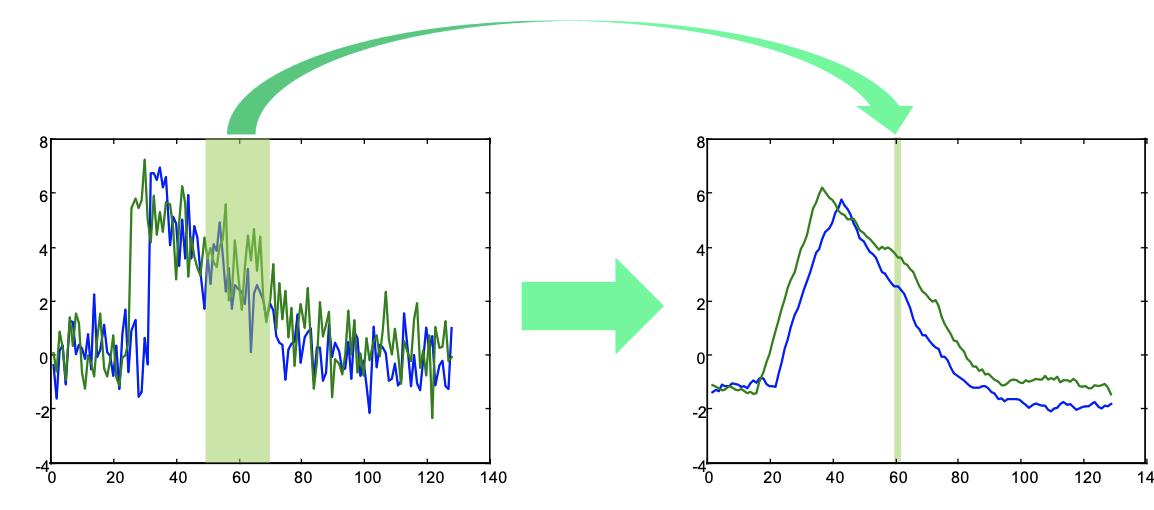
\includegraphics[width=0.9\linewidth]{img/noise_trans.png}
        \caption{Noise transformation.}
        \label{fig:noise-trans}
    \end{figure} \\
    Noise can be removed by a \textbf{moving average} (\textbf{MA}): given a window of length $w$ and a time series $t$, the MA is applied as:
    \begin{equation*}
        t_i = \dfrac{1}{w} \sum_{j=i-w/2}^{w/2} t_j \ i = 1, \dots , n
    \end{equation*}
\end{itemize}

\subsubsection{Dynamic Time Warping}

It's often the case that two time series have approximately the same shape, but they do not line up on the x axis. The euclidean distance calculated between such series would be high, despite them being similar: this is because it considers a fixed time axis for both series. In order to find the similarity between them, the time axis must be ``warped'' for one or both time series to align them correctly.

In practice, DTW is calculated in three steps. First, given the series $Q$ and $C$, a matrix of size $|Q| \times |C|$ is constructed, and each cell of index $i,j$ contains the distance between the $i^{th}$ component of $Q$ and the $j^{th}$ component of $C$. The diagonal of this matrix corresponds to the comparison done by the Euclidean distance. Every possible warping between two time series corresponds to a path from the bottom left corner $(0,0)$ and the top right corner $(0,|C|)$ of the matrix. The DTW will be the best path, i.e., the one that yields the lowest sum of costs. The best path is found recursively, using the following formula:
\begin{equation*}
    \gamma(i,j) = d(q_i,c_j) + \min\{\gamma(i-1, j-1), \gamma(i-1, j), \gamma(i, j-1)\}
\end{equation*}

The dynamic programming approach to the problem starts by calculating the distance matrix for the two series; then, the matrix of cumulative costs for each path; finally, the path with the best alignment is found, connecting the cells with the lowest cost.
\begin{figure}[ht]
    \centering
    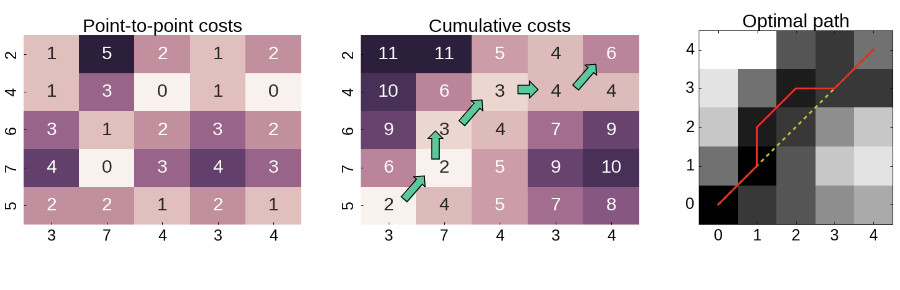
\includegraphics[width=1.0\linewidth]{img/dtw.png}
    \caption{How Dynamic Time Warping is calculated.}
    \label{fig:dtw}
\end{figure}

When the performances of Euclidean distance and DTW are compared for classification tasks, the former leads to much lower accuracy than the latter; however, DTW is also two to three orders of magnitude slower than Euclidean distance, meaning that it is unsuitable for larger datasets if used as is. In order to speed up the calculation of DTW, different approaches can be used depending on the length of the time series.

\begin{itemize}
    \item If the time series are short, then they can be \textbf{approximated} via compression or downsampling; alternatively, computation can be sped up by introducing \textbf{global constraints}.
    
    \item If the time series are long, compression/approximation-based dissimilarity can be used.
\end{itemize}

\paragraph{Global Constraints}

A global constraint limits the indices of the warping path $w_k = (i,j)_k$, such that $j-r \leq i \leq j+r$, where $r$ is an integer that defines the allowed range of warping for a given point in the series. This restricts the computation of distances and cumulative costs to a small window described by $r$. Two types of global constraints are the \textbf{Sakoe-Chiba Band} (restriction around the diagonal) and the \textbf{Itakura Parallelogram} (greater restriction at extremes of series, less restriction in the middle). Empirical analysis shows that given a dataset, the increase in the value of $r$ will rapidly improve performances, but after reaching a maximum they will decrease and then plateau.

\begin{figure}[ht]
    \centering
    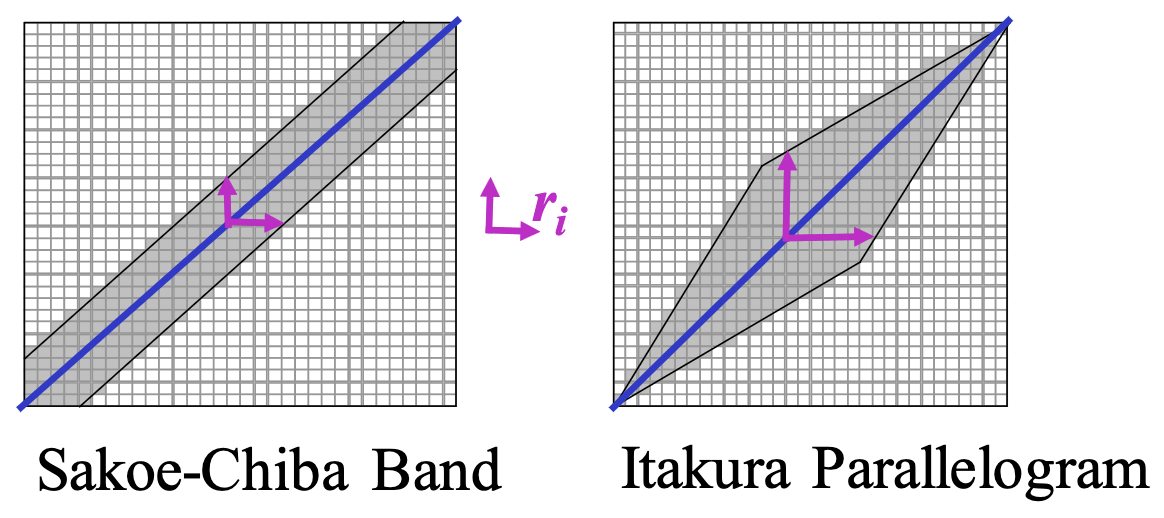
\includegraphics[width=0.7\linewidth]{img/dtw_global_constr.png}
    \caption{Global constraints.}
    \label{fig:dtw-global-constr}
\end{figure}

\paragraph{Approximation}

Approximation is a form of Dimensionality Reduction designed for time series. Compared to compression, approximation maps the series to a smaller space that is understandable, while the compressed space is not necessarily understandable.

\begin{itemize}
    \item \textbf{Discrete Fourier Transform (DFT)}: the time series is represented as a linear combination of sine and cosine functions, but only the first $n/2$ coefficients are kept. Each sine wave only requires 2 numbers: the phase and the amplitude. Many of the coefficients have very low amplitude, so they contribute very little to reconstructed signal: they can be discarded without significant loss of information, saving storage space.

    This approximation works great for most time series that represent natural signals, and many fast ($O(n \log(n))$) implementations exist. However, it struggles with series of different lengths and cannot support weighted distance measures. This approximation loses the temporal information of the original time series.

    \item \textbf{Discrete Wavelet Transform (DWT)}: the time series is represented as a linear combination of wavelet basis functions, but only the first $n$ coefficients are kept. Wavelets represent data in terms of sum and difference of a prototype wavelet, called analyzing/mother wavelet; they are localized in time, so some of the wavelet coefficients will represent small subsections of the data (unlike Fourier coefficients which always represent global contribution to data).

    This approximation has a good ability to compress stationary signals, and many fast ($O(n)$) implementations exist. However, it can only be defined for sequences whose length is an integral power of two; wavelets tend to approximate the left side of the sequence at the expense of the right one; it cannot support weighted distance measures. This approximation loses the temporal information of the original time series.

    \item \textbf{Singular Value Decomposition (SVD)}: the time series is represented as a linear combination of eigenwaves, but only the first $n$ coefficients are kept. This approach is similar to the previous two, but the eigenwaves are extracted from the data and are not a set of default waves.
    
    Time series can be thought of as points in a high-dimensional space, so the axes on which they are represented can be rotated so that axis 1 is aligned with the direction of maximum variance, axis 2 is aligned with the direction of maximum variance and is also orthogonal to axis 1, and so on, until the desired number of axes is obtained. Since the first eigenwaves will capture the most variance in the data, the rest can be truncated with little loss. This approximation loses the temporal information of the original time series.

    \item \textbf{Piecewise Linear Approximation (PLA)}: the time series is represented as a sequence of $k$ straight lines, which can be either connected or disconnected. Each line is described by its length and the height of its leftmost point; the height of the rightmost one can be inferred from the next segment.
    
    This approximation requires to choose the ``best'' value of $k$, that is, the optimal number of segments used to represent the time series that corresponds to the best trade-off between accuracy and compactness; this problem has no general solution.

    This approximation can efficiently compress data and filters noise. It also supports non-euclidean similarity measures.

    \item \textbf{Piecewise Aggregate Approximation (PAA)}: the time series is represented as a sequence of $N$ box basis functions, where each box has the same size. The mean value of the points in each segment is calculated, so that the approximation will be a series made up of several constant lines of fixed length. The dimensionality of the data is reduced from $n$ to $N$ (the number of segments). If $N=1$, the transformed representation is identical to the original series; if $N=n$, the approximation is a single segment equal to the mean of the entire series.

    This approximation is fast to calculate, supports Euclidean and non-Euclidean distance measures, as well as weighted Euclidean distance.
    
    \item \textbf{Adaptive Piecewise Constant Approximation (APCA)}: this approximation was developed as an extension of PAA. It allows the segments in the approximation to have different lengths, so that each segment is represented by two values: the first one corresponds to the mean value of the points falling within the same segment, the second one is its length.

    APCA can place bigger segments for areas of lower activity and many smaller segments for areas with higher activity (hence the ``adaptive''). In general, finding the optimal piecewise polynomial representation of a time series requires a $O(Nn^2)$ dynamic programming algorithm; in practice, however, an optimal representation is not needed, so fast algorithms ($O(n \log(n))$) to calculate high quality approximations exist. It supports Euclidean and non-Euclidean distance measures, as well as weighted Euclidean distance.

    \item \textbf{Symbolic Aggregate Approximation (SAX)}: a time series is \textbf{segmented} using a predefined length $w$, predefined number of segments $k$, or using change point detection methods. SAX converts a time series into a discrete sequence of symbols, using a small alphabet size. Every part of the representation contributes about the same amount of information about the shape of the time series. The series is first normalized, and then two steps of discretization are performed.

    First, the time series of length $n$ is split into $w$ equal-sized segments, and each segment is approximated by the mean of all the points falling in it. Aggregating the resulting $w$ coefficients forms the PAA representation of the time series. Next, the breakpoints that divide the representation into $\alpha$ equiprobable regions are found, where $\alpha$ is the alphabet size (can be set by the user or derived from the Minimum Description Length). These breakpoints are chosen so that the probability of a segment falling into any of the regions is approximately the same: if the symbols were not equiprobable, some substrings would be more probable than others, introducing a probabilistic bias.

    Each region is assigned a different symbol from the chosen alphabet. The PAA coefficients can be mapped to the region to which they reside in a bottom-up fashion: the coefficients that fall in the lowest region are converted to $a$, the ones in the second lowest region to $b$, and so on. At the end, the representation will correspond to a sequence of symbols.
\end{itemize}
\clearpage
\begin{figure}[ht]
    \centering
    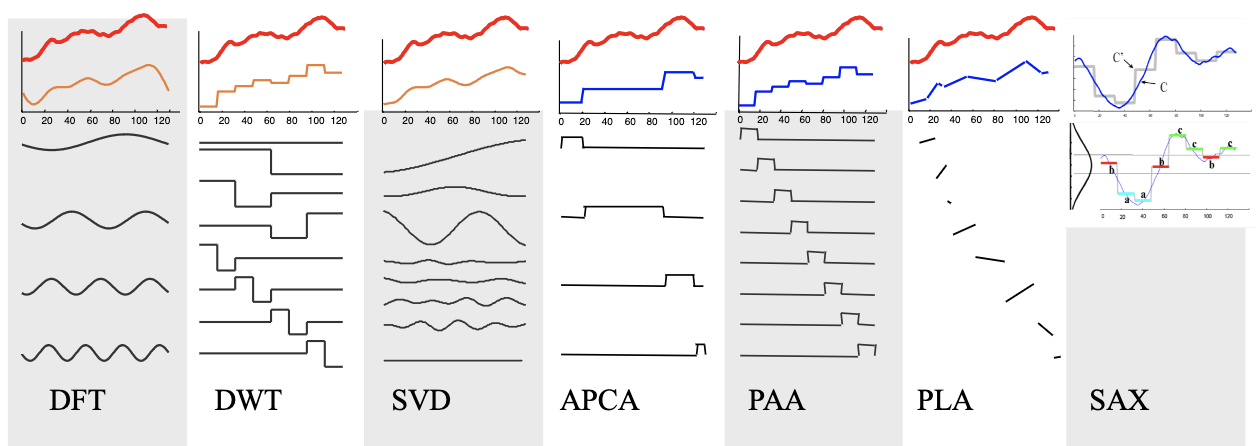
\includegraphics[width=1.0\linewidth]{img/approximations.png}
    \caption{The most common time series approximations.}
    \label{fig:approx-ts}
\end{figure}
\chapter{Time Series: Clustering and Classification}

\section{Clustering}

For time series, the most common methods are Partitional Clustering and Hierarchical Clustering. \textbf{Partitional Clustering} uses the K-means algorithm (or some variant) to optimize the objective function by minimizing the SSE. \textbf{Hierarchical Clustering} starts by computing pairwise distance between time series (using whatever appropriate distance measure is specified by the user), and then merges clusters in a bottom-up way, merging at each step the two closest clusters, until the cluster containing all data points is obtained. This approach is however limited to small datasets, since it is computationally complex.

Time series clustering can be of the following types:
\begin{itemize}
    \item \textbf{Whole clustering}: the conventional type of clustering, where the goal is to assign each data object to a cluster.

    \item \textbf{Feature-based clustering}: features (or motifs, see next section) are extracted from the series, and then used to cluster.

    \item \textbf{Compression-based clustering}: compress time series and run clustering on the compressed versions.

    \item \textbf{Subsequence clustering}: subsequence clustering is done on the subsequences extracted from a single long time series using a sliding window.
\end{itemize}

\section{Motif and Discord Discovery}

\textbf{Motifs} are repeated patterns within a time series. \textbf{Discords} are exceptionally unusual patterns withing a time series. Motif discovery is a preprocessing phase for other analysis: mining association rules, where motifs are referred to as primitive shapes and frequent patterns, classification, which in some cases works by constructing typical prototypes (motifs) of each class, and anomaly detection, in which algorithms use motifs to model typical time series behaviour and detect future patterns that are dissimilar.

Given a predefined motif length $m$, a brute-force approach would simply search all possible motifs obtainable from all possible comparisons of subsequences of length $m$. This approach is clearly inefficient; the most commonly used algorithm was originally developed in bioinformatics, and is based on \textbf{random projections} and SAX.

First, an alphabet size $\alpha$, SAX window size $w$, and motif length $n$ are set. All approximated subsequences of length $w$ are extracted via SAX from the time series by shifting forward the window one measurement at a time, for a total of $|T| - (n - 1)$ subsequences. Then, a mask is randomly chosen to only select certain ``columns'' of the subsequences; i.e., if the mask $\{1,3\}$ is chosen, only the first and third symbols in the representation are considered. Collisions between masked subsequences are recorded with a \textbf{collision matrix}, increasing the value in the corresponding cell. This step is repeated multiple times choosing different masks.

At the end of these random perturbations, motifs can be observed in the collision matrix, looking at the cells that have the highest values: their indexes are the positions in which the motifs start in the time series. The problem with this approach, however, is that it is highly dependent on the approximation technique used.

\subsection{Matrix Profile}

Given a time series $T$, and having calculated the pairwise distance among all the $|T| - (n - 1)$ subsequences that can be extracted from $T$ using a sliding window of length $n$, the \textbf{Matrix Profile} (\textbf{MP}) of a $T$ is the vector that annotates the distance between each subsequence and its nearest neighbor. The index of the corresponding nearest neighbor of each subsequence is stored in a vector called \textbf{Matrix Profile Index}, which can be used to find the nearest neighbor in constant time. Pointers are not necessarily symmetric: if $n$ is the nearest neighbor of $m$, the nearest neighbor of $n$ is not necessarily $m$, but may be some other subsequence. However, for the two smallest values in the MP, the pointers of the corresponding subsequences must be mutual.

\begin{figure}[h]
    \centering
    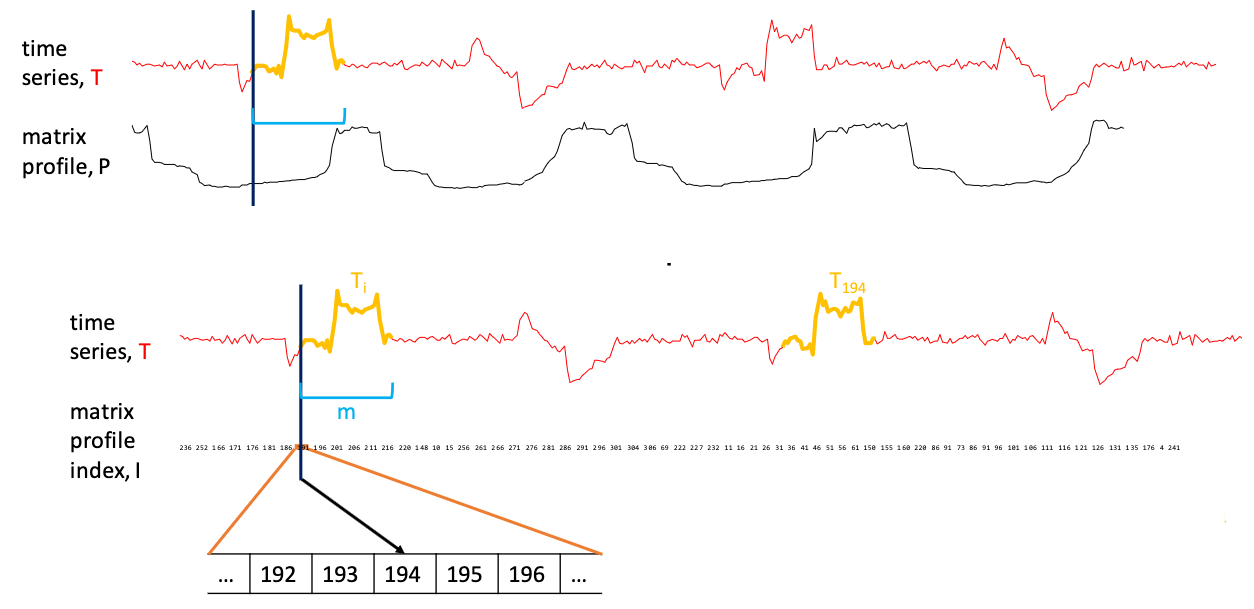
\includegraphics[width=0.9\linewidth]{img/mp_mpi.png}
    \caption{Matrix Profile (on top) and Matrix Profile Index (on the bottom).}
    \label{fig:mp-mpi}
\end{figure}

Low values in the matrix profile indicate that the corresponding subsequence has at least one similar subsequence in the data: these regions indicate motifs. Areas that instead have very high values indicate discords, since they are subsequences whose nearest neighbor is very distant.

To compute the matrix profile of a time series, the cells of the vector are initialized to $\infty$. Then, a random subsequence $T_i$ is selected, and the distance with every other subsequence is stored in a different vector. This step has complexity $O(|T| \log(|T|))$. The matrix profile is updated, applying element-wise minimum to the two vectors (skipping the cell for $T_i$). A new subsequence is randomly selected, and the process is repeated, updating the matrix profile with the new minimum values. The algorithm stops once all subsequences have been selected. The total time complexity is $O(|T|^2 \log(|T|))$.

It may be useful to think of time series subsequences as points in an $m$ dimensional space: subsequences that are very similar will be close together in denser areas, which will in turn correspond to regions in the MP with low values. To understand how the top-k motifs are extracted, we can consider this data-point interpretation. A parameter $R > 1$ is chosen, and the two nearest points are found, called the \textbf{motif pair}. Given the distance $D_1$ between these two points, a circle with radius $D_1 * R$ is drawn around each point: any point that falls within either circles are added to this motif: this is the top-1 motif. To find the top-2 motif, the next closest pair of points is found (excluding the ones in the previous motif), whose distance is $D_2 > D_1$. Again, a circle of radius $D_2 * R$ is drawn around each circle, and all points in this circle are added to the motif. To choose when to stop, i.e., to choose the value of $k$, we can either use a predefined value, or use the Minimum Description Length.

\begin{figure}[h]
    \centering
    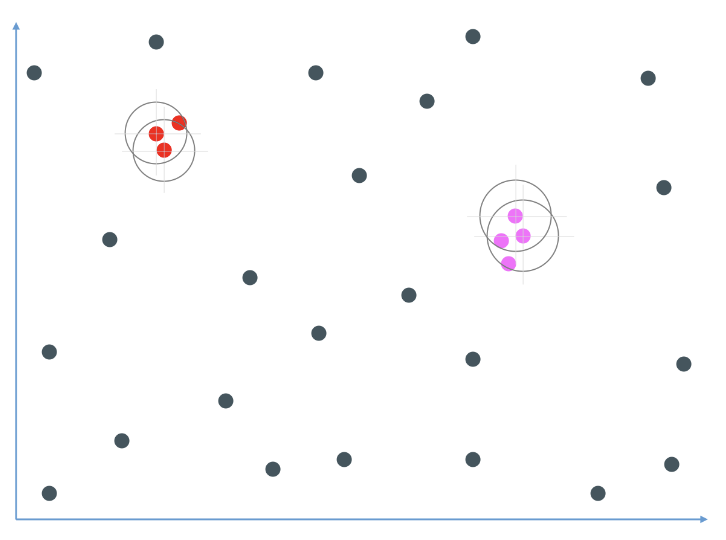
\includegraphics[width=0.5\linewidth]{img/topk_motifs.png}
    \caption{A graphical interpretation of how top k-motifs are found. The red dots are the top 1-motif, and the magenta ones are the top-2 motifs.}
    \label{fig:top-k-motifs}
\end{figure}

If we're interested in finding top-k discords instead, a parameter $E$ is set to select how many subsequences will be excluded in the vicinity of the anomaly, and the subsequence with the highest distance in the MP is found. The $E$ closest subsequences to the anomaly are selected, and removed with the anomaly. Again, the value of $k$ can be either set to a predefined value or chosen as the MDL.

\section{Classification}

For classification tasks, given a set of $n$ time series all assumed of length $m$, each time series $x_i$ is associated with a class label $c_i$. The objective is to find a target function $f$ that maps all possible time series to the space of possible class labels. The most widely used algorithm for time series classification is K-NN, used in the raw data. It is simple, and can be used with Dynamic Time Warping. However, it is a lazy classifier, meaning that prediction is costly as it is, and DTW slows the execution even further. Additionally, K-NN based classification does not provide much insight into the data.

An alternative is shapelet-based classification. \textbf{Shapelets} are time series subsequences that are maximally representative of a class. Once extracted, shapelets can be used to transform the dataset so that it can be used as input for classifiers; additionally, they provide interpretable results, and can be incredibly accurate since they are local features, unlike most other time series classifiers which only consider global features. They also tend to be faster at classification compared to other methods, since the time complexity of the prediction phase is only $O(ml)$, where $m$ is the length of the query time series, and $l$ is the length of the shapelet. In contrast, DTW-based K-NN has a time complexity of $O(km^3)$, where $k$ is the number of objects in the training set.

Since shapelets are much shorter than the time series they're extracted from, we need to define a measure to evaluate the similarity between a subsequence and a time series. The distance between two time series $T$ and $S$, with $|S| < |T|$, is calculated via:
\begin{equation*}
    SubsequenceDist(T,S) = \min(Dist(S,S')) \ \forall S' \in S_T^{|S|}
\end{equation*}
where $S_T^{|S|}$ is the set of all possible subsequences of $T$. This function returns the distance between $S$ and the ``best matching'' location in $T$. Each time series in a dataset can be represented as a vector of distances with the shapelets extracted from them: if a given time series belongs to a certain class, it will be very close to the representative shapelet(s) of that specific class, and further away from shapelets that represent other classes.

\begin{figure}[h]
    \centering
    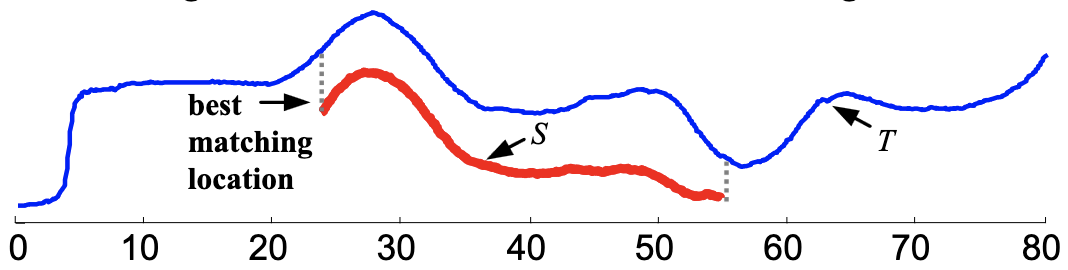
\includegraphics[width=0.5\linewidth]{img/subsequencedist.png}
    \caption{The best matching location of $S$ over $T$.}
    \label{fig:subseq-dist}
\end{figure}

\subsection{Shapelet Extraction}

The simplest way to extract shapelets is the brute-force approach, which generates all possible subsequences of all possible lengths from the time series in the dataset, adding them to the pool of candidates. Assume the time series are each assigned to one of two possible class labels. For each candidate, the algorithm must check how well it separates the objects of one class from the other, and choose the candidate that performs best. First, all time series are rearranged in the dataset based on the distance from the current candidate; then, the optimal split point that maximizes the \textbf{information gain} is found, similarly to how splits are chosen in Decision Tree training algorithms. After calculating the information gain of all candidates, the one with the highest value is selected.

A common measure used to evaluate information gain is entropy:
\begin{equation*}
    I(D) = -p(A) \log_2 (p(A)) -p(B) \log_2 (p(B)) \,,
\end{equation*}
where $p(A)$ and $p(B)$ are the proportion of objects belonging to each respective class $A$ and $B$. Given a strategy that divided the dataset $D$ into two subsets $D_1$ and $D_2$, the information remaining in the dataset after the split is calculated as the weighted average entropy of each subset.
If the fraction of objects in $D_1$ is $f(D_1)$, and the fraction of objects in $D_2$ is $f(D_2)$, the total entropy of the dataset after a split is calculated as:
\begin{equation*}
    \hat{I}(D) = f(D_1)I(D_1) + f(D_2)I(D_2)
\end{equation*}
The information gain for a splitting rule is given by the difference of the entropy before and after the split:
\begin{equation*}
    Gain(split) = I(D) - \hat{I}(D)
\end{equation*}

The total number of candidates generated by the brute-force approach amounts to:
\begin{equation*}
    \sum_{l = minlen}^{maxlen} \sum_{T_i \in D}(|T_i| - l + 1)
\end{equation*}
Then, for each of these candidates, the distance with every training time series must be calculated, as well as the entropy for each split. Obviously, this solution is highly space and time inefficient; two speedup methods are:
\begin{itemize}
    \item \textbf{Distance Early Abandon}: in the brute-force approach, the distance from the time series $T$ with the subsequence $S$ is done by calculating the Euclidean distance between each subsequence of length $|S|$ in $T$ and $S$, and choosing the minimum. This operation costs $O(|T|)$. However, the only distance we need is the one we keep, i.e., the minimum one. Instead of calculating all distances, the calculations can stop after the distance starts to increase compared to the smallest value recorded so far; this technique is known as early abandon.

    \item \textbf{Admissible Entropy Pruning}: we want to find only the best shapelet for each class. Obtaining the distance between a candidate and its nearest matching subsequence in each time series in the dataset is the most expensive operation. Instead of waiting until all distances from all time series are calculated, an upper bound of the information gain can be calculated based on the distances known so far. If at any point this upper bound cannot beat the best-so-far information gain, the distance calculations are stopped, pruning the candidate, since there's no way it could ever be better than the best candidate found so far. This is done by comparing the information gain of the best candidate with the information gain of the current one where all training instances that haven't been compared yet are assumed to be perfectly classified. 
\end{itemize}




\chapter{Imbalanced Learning}

Most classification tasks assume that classes are equally represented withing the training set. In reality, it's very common to have a majority (negative) class and a minority (positive) class, of which the latter contains only a small fraction of the training data, since it represents a set of more interesting events/objects. In order to handle imbalanced data, we can follow these approaches:
\begin{itemize}
    \item \textbf{Do nothing}: ?
    \item \textbf{Balance the training set}: the training set is modified, using either under- or oversampling.
    \item \textbf{Balance at the algorithm level}: the algorithm is modified, adjusting the weight associated to the classes, using a different decision threshold, or using specific algorithms that perform well on imbalanced data.
    \item \textbf{Switch to Anomaly Detection}: ?
\end{itemize}

\section{Balancing the Training Set}

\subsection{Undersampling}

\textbf{Undersampling} is done on the majority class to reduce its size and make it comparable to that of the minority class. The simplest way is using \textbf{random undersampling}, with or without replacement, simply randomly selecting elements from the majority class until a set of the desired size is obtained.

Another technique is \textbf{Tomek Links}: it selects pairs of examples $(a,b)$ that respect the following properties:
\begin{itemize}
    \item $a$ is the nearest neighbor of $b$;
    \item $b$ is the nearest neighbor of $a$;
    \item $a$ and $b$ belong to different classes.
\end{itemize}
From this pair, the element belonging to the majority class is removed from the dataset. This way, all samples from the majority class that are very close to those in the minority class (i.e., they're harder to distinguish) can be excluded from the dataset.

\textbf{Edited Nearest Neighbor} works as follows: for each example, it finds its k-nearest neighbors, and checks the predicted class by that neighborhood; if this predicted class does not match the class of the example, it is removed along with the neighborhood. At the end, all examples that were too close to instances of the opposite class will have been removed from the dataset.

\textbf{Condensed Nearest Neighbor} performs a smart undersampling, constructing the subset of records which are able to correctly classify the original data using $k$-NN (typically, $k$ is set to 1). The algorithm operates using these steps:
\begin{enumerate}
    \item A random example is extracted and added to \texttt{STORE}. All other records are added to \texttt{GRABBAG}.
    \item A loop iterates over all other samples in the dataset; for each example, it is classified via $k$-NN using the contents of \texttt{STORE}, and, if the prediction does not match the class label, it is moved to \texttt{STORE}. The loop continues until either \texttt{GRABBAG} becomes empty or a whole pass over it is done without no transfers to \texttt{STORE}.
    \item Return \texttt{STORE}.
\end{enumerate}

Finally, undersampling can be done by first performing centroid-based clustering on the data representing the majority class, and then using only the centroids instead of the entire data.

\subsection{Oversampling}

\textbf{Oversampling} the minority class increases the amount of examples belonging to it. Oversampling can also be done with random sampling, with or without replacement, as seen for undersampling.

\textbf{SMOTE} (Synthetic Minority Oversampling TEchnique) oversamples the minority class by adding data points via interpolation. It operates in the feature space, introducing synthetic examples along the segments that connect each sample with any/all of its minority class $k$ nearest neighbors. Depending on the amount of oversampling needed, the value of $k$ can be changed (by default, $k=4$). In practice, interpolation is done by taking the difference between the current sample and one of its neighbors; this difference is multiplied by a random number between 0 and 1, and the result is added to the values of the current sample. The final record represents a point that is somewhere along the segment that connects the sample and the neighbor.

An alternative to SMOTE is \textbf{ADASYN} (ADAptive SYNthetic). This algorithm operates as follows:
\begin{enumerate}
    \item The ratio of min to maj class examples is calculated as $d = \#min/\#maj$.

    \item The total number of synthetic minority class examples as $G = (\#maj - \#min) / \beta$, where $\beta$ is the desired ratio of minority.

    \item The $k$-NN of each minority sample is found, and the ratio of majority class examples is found for that neighborhood as $r_i = \#maj_i / k$; this ratio is then normalized by dividing it by the sum of all the $r_i$.

    \item The number of synthetic samples to generate for each neighborhood is calculated as $G_i = G_{r_i}$.

    \item $G_i$ samples are generated for each neighborhood, taking two minority samples $(x_i, y_i)$ within the neighborhood, and interpolating among them (as SMOTE does).
\end{enumerate}

\section{Balancing at the Algorithm Level}

Another way to handle unbalanced data is to modify the behaviour of the training algorithm to take into account the disparity between the classes. There's two main ways this can be done: using class weights, or adjusting the decision threshold.

The overall performances of a classifier can be summarized using a confusion matrix. A corresponding \textbf{cost matrix} can be constructed, associating a different cost (weight) to each ``event''.

\begin{figure}[H]
\centering
\begin{minipage}{0.49\textwidth}
    \begin{tabular}{|c||c|c|}
         \hline
         & pred. + & pred. - \\
        \hline
        \hline
        actual + & $f_{++}$ & $f_{+-}$\\
        \hline
        actual - & $f_{-+}$ & $f_{--}$\\
        \hline
    \end{tabular}
\end{minipage}
\hfill
\begin{minipage}{0.49\textwidth}
    \begin{tabular}{|c||c|c|}
         \hline
        $C(i|j)$ & pred. + & pred. - \\
        \hline
        \hline
        actual + & $C(+|+)$ & $C(-|+)$\\
        \hline
        actual - & $C(+|-)$ & $C(-|-)$\\
        \hline
    \end{tabular}
\end{minipage}
\caption{Confusion matrix on the left, cost matrix on the right.}
\end{figure}
The objective of the training algorithm is to minimize the total cost given by:
\begin{equation*}
    \sum_X C_X * freq_X
\end{equation*}
There's some classifiers, called \textbf{Meta-Cost Sensitive Classifiers}, that calculate the risk of classifying a certain instance $x$ as class $i$:
\begin{equation*}
    R(i|x) = \sum_j P(j|x)C(i,j)
\end{equation*}

Many classifiers predict what class an instance belongs to by computing scores that represent the probability that the given instance belongs to a class. The score is usually the probability that the instance belongs to the positive/minority class. By default, if the score is greater than 50\%, the instance is predicted as positive, otherwise it is predicted as negative. This schema can be generalized: if the score is greater than some threshold $THR$ the instance is classified as positive, otherwise it is negative. For each possible threshold, we will get a different set of predictions, and all associated metrics change as well (accuracy, precision, recall, etc.).

To monitor how changing this threshold influences the behaviour of the model, it can be useful to study the \textbf{Receiving Operating Curve} of the model, which plots the True Positive Rate against the False Positive Rate for different values of the threshold.
\chapter{Dimensionality Reduction}

Dimensionality reduction is the process of reducing the number of variables in the dataset, obtaining a set of \textbf{principal variables}. Approaches for dimensionality reduction can be divided into feature selection and feature projection.

\section{Feature Selection}

\textbf{Feature selection} extracts a subset of the variables via different strategies: \begin{itemize}
    \item \textbf{Filter strategy}: the relevance of each feature is evaluated using some appropriate measure (e.g., Information Gain), removing the ones whose corresponding value falls below a given threshold. Commonly, a variance threshold is used. By default, it removes all zero-variance features, meaning the ones that have a constant value. Another technique is Univariate Feature Selection, which selects the best features based on univariate statistical tests. An example of statistical test is the ANOVA F-Value between dependent and independent variables:
    \begin{equation*}
        \textit{F-value} = \dfrac{\sum_{i=1}^K n_i(\bar{Y}_i - \bar{Y})^2 / (K-1)}{\sum_{i=1}^K \sum_{j=1}^{n_i} (Y_{ij} - \bar{Y}_i)^2 / (N-K)} \,,
    \end{equation*}
    where $Y_i$ is the sample mean over the $i^{th}$ group, $n_i$ is the number of observations in the $i{th}$ group, $\bar{Y}$ is the overall mean, $Y_{ij}$ is the $j^{th}$ observation in the $i^{th}$ out of $K$ groups, and $K$ and $N$ are the number of groups and the sample size, respectively. The F-value is large when the numerator is large, which is unlikely if the population means of the groups have the same value;

    \item \textbf{Wrapper strategy}: the performances of different subsets of features are compared using a model (e.g. a classifier of which we evaluate accuracy), and the subset that yields the best result is selected. An example is Recursive Feature Elimination (RFE), which selects features by recursively considering smaller and smaller sets of features: first, an estimator is trained on the data, and the ``importance'' of each feature is returned. The least important features are pruned from the current set in a recursive fashion, until the desired number of features to select is reached.

    \item \textbf{Embedded strategy}: feature selection is done at the algorithm level, where parameters are modified and appropriate weights are assigned to each feature.
\end{itemize}

\section{Feature Projection}

\textbf{Feature projection} transforms the features via either linear or non-linear transformations. The most common approaches include:
\begin{itemize}
    \item Random Subspace Projection;

    \item Principal Component Analysis (PCA) and Singular Value Decomposition (SVD);
    
    \item Multidimensional Scaling (Sammon maps, ISOMAP, t-SNE);

    \item Non-negative Matrix Factorization (NMF);

    \item Linear Discriminant Analysis (LDA);

    \item Autoencoders.
\end{itemize}
Random Subspace Projection is a very simple approach: the data is projected into low-dimensional space using a random matrix whose columns have unit length. It preserves the structure of the data, and is computationally cheap.

\subsection{Principal Component Analysis (PCA)}

The goal of \textbf{Principal Component Analysis} is to find a new set of attributes that better capture the variability of the data; the first dimension is chosen as the one that captures as much of the variability as possible, the second one as the dimension that is orthogonal (uncorrelated) to the first and also captures the most of the remaining variability in the data, and so on until the number of desired dimensions is reached. These dimensions are obtained via linear transformations of the original attributes. The steps of PCA are the following:
\begin{enumerate}
    \item The dataset $X$ is standardized.
    
    \item The mean value of data is calculated across each dimension.
    
    \item The covariance matrix of all pairs of features is calculated; given a matrix of data $X$, the mean of each column is removed from the column vectors to get the centered matrix $C$, and so the covariance matrix of the row vectors of $X$ is calculated as $\Sigma = C^TC$.
    
    \item The eigenvalues and eigenvectors of $\Sigma$ are found, and the $k$ eigenvectors corresponding to the largest eigenvalues are chosen.
    
    \item The original dataset is transformed using the eigenvectors found in the previous step as the new axes.
\end{enumerate}
Once the dataset has been transformed, any reconstruction will have some error.

The covariance matrix is used to store the covariance between each pair of attributes in the dataset. The diagonal of the matrix contains the variance of each attribute (since the covariance of a variable with itself is its variance). Since this matrix is symmetric, its eigenvectors are guaranteed to be orthonormal.

In order to compute the eigenvalues and eigenvectors of the covariance matrix, \textbf{Singular Value Decomposition} is often used. A matrix $A \in R^{m \times n}$ can be written as:
\begin{equation*}
    A = U \Sigma V^T \,,
\end{equation*}
where $\Sigma$ is the diagonal of $A$, and the columns of $V$ are the eigenvectors of the covariance matrix, sorted from largest to smallest eigenvalues.

\subsection{Multi-Dimensional Scaling (MDS)}

Given a pairwise dissimilarity matrix, the goal of MDS is to learn a mapping of data into a lower dimensional space such that the relative distances are preserved. These methods are used to map data to very low configurations (e.g., 2 or 3 dimensions).

The key steps of MDS are the following:
\begin{enumerate}
    \item Given a pairwise dissimilarity matrix $D$, and the dimensionality $k$, find a mapping such that $d_{ij} = \|x_i - x_j\|$ for all points in $D$.

    \item The function
    \begin{equation*}
        J(x) = \sum_{i=1}^n \sum_{j=1}^n d_1 (d_{ij}, d_2(x_i, x_j))
    \end{equation*}
    is minimized, usually via a gradient descent algorithm, solving the associated optimization problem.
\end{enumerate}
Depending on the distances used, the approach will return a different result. Classic MDS uses Euclidean distances for every calculation, Metric-MDS uses metrics as distances, and Non-Metric-MDS uses ranks of distances instead of their values.

\textbf{Sammon Mapping} is an algorithm that, similarly to MDS, maps the data to a lower dimensional space while trying to preserve relative distances. It can be seen as a generalization of Metric-MDS. It introduces a weighting system that normalizes the squared errors in pairwise distances using the distance in the original space:
\begin{equation*}
    J(x) = \sum_{i=1}^n \sum_{j=1}^n \dfrac{d_1 (d_{ij}, d_2(x_i, x_j))}{d_{ij}}
\end{equation*}
As a consequence, Sammon Mapping preserves the small $d_{ij}$, making them more ``important'' in the fitting procedure than larger distances. In general, Sammon mapping better preserves inter-distances for smaller dissimilarities, and proportionally squeezes the inter-distances for larger dissimilarities.

\textbf{ISOmetric Feature MAPping} (\textbf{ISOMAP}) is used for dimensionality reduction when the data points have a complicated, non-linear relationship to one another; it preserves the intrinsic geometry of the data. The basic ISOMAP algorithm is:
\begin{enumerate}
    \item For each data point, the nearest neighbors are found using Euclidean distance. These neighborhood relationships are represented as a weighted graph $G$, where each link between nodes $u$ and $v$ has a weight that corresponds to the distance between $u$ and $v$.

    \item The geodesic distance between all pairs of points on the data manifold is calculated by computing the shortest path distances on the graph $G$.

    \item An embedding of the data in a $k$-dimensional Euclidean space is constructed. This embedding is the one that best preserves the manifold geometry.
\end{enumerate}

\textbf{t-Distributed Stochastic Neighbor Embedding} (\textbf{t-SNE}) is mostly used for data visualization. While PCA tries to find a global structure, t-SNE tries to preserve local structure, i.e., distances and neighbors are preserved by the mapping. SNE encodes high dimensional neighborhood information as a distribution.

For each input data point $x_i$, imagine we have a Gaussian distribution centered around it. The probability that $x_i$ chooses another data point $x_j$ as its neighbor is proportional with the density under this Gaussian: if the standard deviation is high this probability is low, and vice-versa. This probability is calculated as:
\begin{equation*}
    p_{j|i} = \dfrac{e^{-\frac{\|x_i - x_j\|^2}{2 \sigma_i^2}}}{\sum_{k \neq i} e^{-\frac{\|x_i - x_k\|^2}{2 \sigma_i^2}}}
\end{equation*}
The final distribution over pairs is symmetrized: $p_{ij} = 1 / 2N(p_{ij} + p_{ji})$. For each distribution $p_{j|i}$, we define the \textbf{perplexity}:
\begin{equation*}
    \textit{perp}(p_{j|i}) = 2^{H(p_{j|i})} \,,
\end{equation*}
where $H(p)$ is the entropy. If the distribution is uniform over $k$ elements, the perplexity is $k$; if the perplexity is low, the sigma is small, while if the perplexity is high the sigma is large.

The objective of SNE can be defined as: given a dataset $x_1, \dots, x_n \in R^m$, defined the distribution $p_{ij}$, find a good embedding $y_1, \dots, y_n \in R^k, k < m$, such that
\begin{equation*}
    q_{j|i} = \dfrac{e^{-\|y_i - y_j\|^2}}{\sum_{k \neq i} e^{-\|y_i - y_k\|^2}}
\end{equation*}
is optimized to be the closest possible to $p$, minimizing the \textbf{KL-divergence}. KL-divergence measures the distance between two distributions $P$ and $Q$, as:
\begin{equation*}
    C = \sum_i KL(P_i | Q_i) = \sum_i \sum_j p_{j|i} \log(\frac{p_{j|i}}{q_{j|i}})
\end{equation*}
This is not a metric function, since it's not symmetric. It measures the penalty for using a wrong distribution, and is usually minimized using gradient descent. This is not a convex problem, so there's no guarantee an optimum will be reached, but multiple restarts can be done attempt at finding a good enough solution.

The peculiarity of t-SNE is that for $Q$, instead of using a Gaussian distribution, it uses a heavy tailed distribution:
\begin{equation*}
    q_{ij} = \dfrac{(1 + \|y_i - y_j\|^2)^{-1}}{\sum_{k \neq l} (1 + \|y_k - y_l\|^2)^{-1}}
\end{equation*}

\chapter{Outlier Detection}

An \textbf{outlier} (anomaly) is an observation that doesn't fit the distribution of the data for normal instances, i.e., is unlikely under the distribution of the majority of instances. Outlier (anomaly) detection has the goal of finding these anomalies in datasets. Although outliers are by definition unusual, their discovery and analysis may provide critical insights on the data, in applications like fraud detection, intruder detection, ecosystem disturbances, medicine and public health, aviation safety, and so on. In all these fields, finding exceptional events or objects is often the main focus of analysis: in fraud detection we're interested in finding anomalous credit card transactions; in intrusion detection attacks can be identified by noticing weird behaviour in systems and networks.

Outliers can be caused by natural variation in values or data belonging to a minority class, or may be caused by errors. In comparison, \textbf{noise} is a random error addition to data typically caused by imprecision during measurements; it does not necessarily produce unusual values or objects, and is normally not interesting per se. Also, data objects may be outliers only for some attributes, or considering all of them. Identifying outliers in a multivariate setting can be challenging, especially when the dimensionality is high.

There are two ways in which an outlier detection method can be used. In the first one, given a dataset with both normal and anomalous instances, we are required to identify these anomalies. In the second one, we're also provided a test set of instances which we want to classify as either outliers or normal data objects. All the techniques presented in the next section can operate in the first way, and most of them (with a few exceptions) can operate in the second way.

\section{Characteristics of Outlier Detection Methods}

\begin{itemize}
    \item \textbf{Model-based vs. Model-free}: many approaches build actual models that can be used to identify whether a test instance is anomalous or not. Most \textbf{model-based} techniques construct a model trained on the normal class and identify any data point that does not fit the model. Alternatively, a model can be trained on both normal and anomalous data, and outliers are identified as those data points which are more likely to belong to the anomalous class. Both cases don't necessarily need label data (i.e., models can be trained in an unsupervised way), since they can make assumptions about the nature of the anomalous class.

    On the other hand, \textbf{model-free} approaches don't explicitly construct a model that characterizes the distribution of the anomalous and/or normal class. Instead, they directly identify instances as outliers without the need for any training, using a simpler calculation.

    If the ground truth of anomalies is available, we could define a classification problem to find outliers and solve it using popular machine learning models (ensemble models, support vector machines, deep neural networks,...). The dataset would often be unbalanced, so ad-hoc formulations should be adopted.

    \item \textbf{Global vs. Local}: some approaches consider the global context, building a model or computing an output considering the entire dataset, or by only considering the local context of each data instance; specifically, an outlier detection approach is local if its output on a given instance does not change if instances outside the local neighborhood of that point are modified or removed.

    Some approaches may be both, either because the reference set for an instance varies automatically during execution, or because it can be set by an hyperparameter.

    \item \textbf{Label vs. Score}: different approaches produce outputs in different formats. Some produce a binary \textbf{anomaly label}, and each object is identified as either an outlier or a normal instance. Others produce an \textbf{anomaly score}, indicating how strongly an instance is likely to be an anomaly. After calculating the score of a set of instances, a ranking can be obtained to identify the top-most scoring anomalies. Optionally, a cut-off threshold can be set so that all instances with a score above that are definitely classified as outliers, while the ones below are normal instances.
\end{itemize}
A very simple visual technique to find outliers is using boxplots and scatterplots. However, they do not return explicit values, and are highly subjective, since they cannot find points that are outliers when considering all dimensions. An alternative is calculating the \textbf{Histogram-based Outlier Score}, which is done by building histograms for each feature. These histograms are then normalized to the $[0,1]$ range, and the \textbf{HBOS} for each record $p$ is computed as a product of the inverse of the estimated density (according to the histograms):
\begin{equation*}
    \textit{HBOS}(p) = \sum_{i=0}^d \log(\dfrac{1}{\textit{hist}_i(p)})
\end{equation*}
This approach assumes that features are independent.

\section{Statistical Approaches}

Statistical approaches use probability distributions to model the normal class, associating a probability value to each data instance indicating how likely it is for that instance to be generated from that distribution. Outliers will be all instances with an associated low probability.

In practice, it applies a statistical test that depends on data distribution, parameters of the distribution (mean, variance, etc.), and the number of expected outliers (a confidence limit). One of the main issues in these approaches lies in identifying the distribution of a dataset (which is not known a priori), considering that often datasets have a mixture of distributions. These approaches are also influenced by the number of attributes in the data.

\textbf{Grubb's Test} detects outliers in univariate data. It assumes a normal distribution. One outlier is detected at a time and removed from the dataset, using a statistical test: the null hypothesis $H_0$ is \textit{``there is no outlier in the dataset''}, while the alternative hypothesis $H_A$ is \textit{``there is at least one outlier in the dataset''}. The Grubb's test statistic is:
\begin{equation*}
    G = \dfrac{\max |X - \bar{X}|}{s} 
\end{equation*}
with $\bar{X}$ being the sample mean and $s$ the sample standard deviation of the data.
The null hypothesis is rejected at significance level $\alpha$ if:
\begin{equation*}
    G > \dfrac{N-1}{\sqrt{N}} \sqrt{\dfrac{t^2_{\alpha/N, N-2}}{N-2+t^2_{\alpha/N, N-2}}}
\end{equation*}
where $t_{alpha/N, N-2}$ is the upper critical value of the t-distribution with $N-2$ degrees of freedom and a significance level of $\alpha/N$. This is a one-sided test, but it can be defined as a two-sided test by using $\alpha/2N$.

Another approach is based on \textbf{likelihood}. Assume the dataset contains samples from a mixture of two probability distribution, $M$ (majority) and $A$ (anomalous), such that $D = (1-\lambda)M + \lambda A$. Initially, all points are assumed to belong to $M$. Let $L_t(D)$ be the log likelihood of the dataset at time $t$; for each data point $x_t$ that belongs to $M$, it is moved to $A$, and the following check is done:
\begin{itemize}
    \item Calculate $L_{t+1}(D)$, the new log-likelihood of the dataset.
    \item Compute $\Delta = L_t(D) - L_{t+1}(D)$.
    \item If $\Delta > c$ ($c$ is a user-defined threshold), then $x_t$ is declared an outlier and permanently moved to $A$. Otherwise, it is moved back to $M$.
\end{itemize}

\paragraph{Pros} statistical approaches have a firm mathematical foundation, can be very efficient, and produce good results if the data distribution is known.

\paragraph{Cons} in many cases, the data distribution is unknown, and for high-dimensional data estimating it may be difficult, therefore the assumptions done by these approaches may be completely incorrect. Also, these are global approaches, and anomalies distort the parameters of the distribution.

\section{Deviation-based Approaches}

Given a set of data points, outliers are those which do not fit to the general characteristics of that set, i.e, the variance of the set is minimized if those outliers are removed from it. This idea is at the basis of deviation-based approaches, which assume that outliers are the outermost points.

An example of such approach is the one proposed in \cite{arning1996linear}, where the problem is defined as follows. Given:
\begin{itemize}
    \item A set of items $I$;
    \item A dissimilarity function $D$;
    \item A cardinality function $C$, such that $I_1 \subset T_2 \implies C(I_1) < C(I_2)$ for all $I_1, I_2 \subseteq I$;
\end{itemize}
Define for each $I_j \subset I$ the \textbf{smoothing factor}:
\begin{equation*}
    SF(I_j) = C(I-I_j) * (D(I) - D(I-I_j))
\end{equation*}
Then, we say that $I_x \subset I$ is an \textbf{exception set} with respect to $D$ and $C$ if
\begin{equation*}
    SF(I_x) \geq SF(I_j) \forall I_j \subset I
\end{equation*}
Intuitively, the exception set contains all instances that contribute the most to the dissimilarity of the itemset $I$ with the least number of elements; in other words, its outliers. The smoothing factor indicates how much the dissimilarity can be reduced by removing the subset $I_j$ from $I$. 

This approaches is similar to statistical-based ones, although it does not depend from a chosen distribution. The naive solution is in $O(2n)$ for $n$ data objects, and can be applicable to any data type. It often applies an heuristic such as random sampling or best first search. It outputs a labeling.

\section{Depth-based Approaches}

Depth-based approaches search for outliers at the border of the data space. Instances are first organized in convex hull layers, and outliers are points that lie in the outermost layers, while normal points are those which lie in the center of the data space, therefore in the innermost layers.

The figure below shows an example dataset.
\begin{figure}[h]
    \centering
    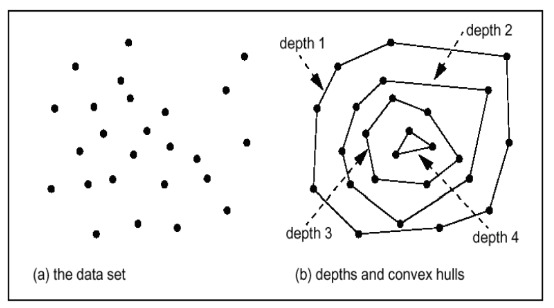
\includegraphics[width=0.5\linewidth]{img/depth_based_od.png}
    \caption{Example of depth-based outlier detection.}
    \label{fig:depth-od}
\end{figure} \\
The points on the convex hull of the full dataset have depth 1. The points in the convex hull of the dataset obtained by removing the points of depth 1 have depth 2, and so on. Once a certain number of convex hulls have been calculated, all points with a depth smaller than some hyperparameter $k$ are reported as outliers. By default it produces a label, but it can be modified so that it returns the depth of each point instead of a 0/1 classification. This algorithm, however, is typically only efficient for two- or three-dimensional spaces. 

Another depth-based algorithm is \textbf{Elliptic Envelope}. It finds the center of the data samples and draws an ellipsoid around it, creating an imaginary elliptical area around the dataset. Instances that fall inside the envelope are considered normal, and anything outside is an outlier. This algorithm works best for data with a Gaussian distribution.

\section{Proximity-based Approaches}

\subsection{Distance-based}

A simple way to define the anomaly score of an instance $x$ is to use its distance to the $k^{th}$ nearest neighbor, $\textit{dist}(x,k)$. If an instance has a lot of close points (so it belongs to the group of normal data), this distance will be small, otherwise the point will be far away from the rest and have a very high distance compared to the rest. Outlier detection algorithms which use $k$-NN distances to score data follow two approaches: either they have a simple \textbf{nested-loop} structure, where a sequential scan computes the $k$-NNs of each instance, or they are \textbf{partition-based}, i.e., they first partition data into micro clusters, and information is aggregated for each partition. This way, micro clusters that cannot qualify when searching for the $k$-NNs of a point can be pruned.

Another common algorithm uses two parameters, a radius $\varepsilon$ and a percentage $\pi$, such that a point $p$ is considered an outlier if at most $\pi$ percent of all other points have a distance to $p$ less than $\varepsilon$ ($p$ is close to very few points). Formally, the set of outliers is computed as:
\begin{equation*}
    \textit{OutlierSet}(\varepsilon, \pi) = \left\{ p | \dfrac{\#\{q \in D | \textit{dist}(p,q) < \epsilon}{\# D} \leq \pi \right\}
\end{equation*}

Finally, outliers can be identified using the \textbf{in-degree number}. Given a dataset, the $k$-NN graph is constructed: each vertex is a data point, and each directed edge between two vertices $p$ and $q$ means that $q$ is one of $p$'s k-nearest neighbors. The in-degree of a point is calculated as the number of reverse $k$-NNs (R$k$-NN), i.e., the number of points who have it as a neighbor. If a point has an in-degree lower than some user-defined threshold, it is declared an outlier. This algorithm outputs an outlier label.

\paragraph{Pros} Distance-based approaches are very simple to implement. They do not require any training, since they're model-free.

\paragraph{Cons} Since the outcome depends on distances, they tend to be slow, and they're not as accurate in high-dimensional spaces. Also, they're sensitive to the chosen hyperparameters and to variations in density.

\subsection{Density-based}

The density around an instance can be defined as $n/V(d)$, where $n$ is the number of instances within a given distance, and $V(d)$ is the volume of the neighborhood. Since $V(d)$ is constant for a given $d$, the density is often only represented using $n$ after fixing a value of $d$. Outliers can be defined as points that are in regions of low density, and their anomaly score as the inverse of the density around them (or the inverse of distance to the $k^{th}$ distance, or the inverse of the average distance to $k$ neighbors). However, if the dataset has regions of different density, this approach can present problems (as seen when discussing DBSCAN).

To fix this problem, the \textbf{average relative density} can be used instead. Given a point $x$ and a number of neighbors $k$, it is calculated as:
\begin{equation*}
    \textit{avg. relative density}(x,k) = \dfrac{\textit{density}(x,k)}{\sum_{y \in N(x,k) \textit{density}(y,k)/|N(x,k)|}}
\end{equation*}
where $N(x,k)$ is the $k$-nearest neighbor of $x$. This way, the density around a point depends on that of its nearest neighbors. If the dataset has areas with differing densities, points in lower density areas will not be classified as outliers. If a point is so faraway that its normal density is high, this relative density will also be high. However, if a point is an outlier only for a very dense cluster, it may not be identified (such as the situation in the figure below).
\begin{figure}[h]
    \centering
    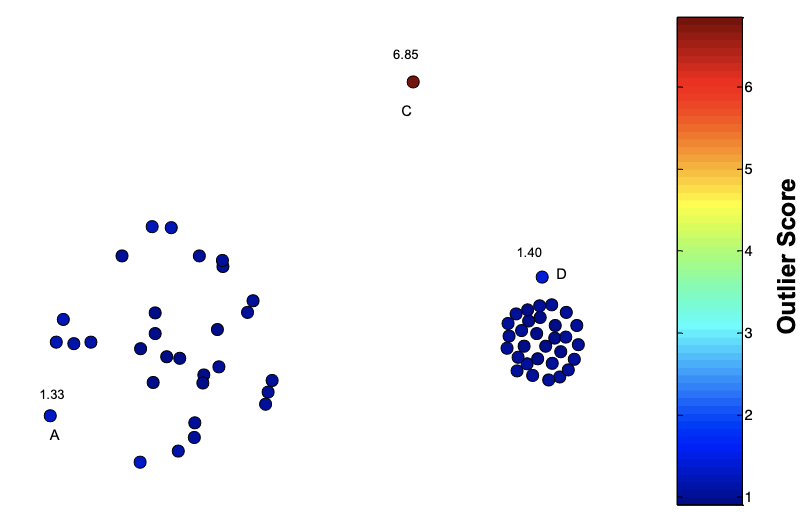
\includegraphics[width=0.5\linewidth]{img/relative_density.png}
    \caption{An example in which average relative density fails. Notice how point $D$ is an outlier for the denser cluster, but it is treated as a normal point.}
    \label{fig:relative-dist}
\end{figure}

\subsubsection{Local Outlier Factor (LOF)}

An alternative is using the \textbf{Local Outlier Factor} (\textbf{LOF}). First, for each pair of points $p$ and $o$ in the dataset, their \textbf{reachability distance}is calculated, identical to that used in OPTICS:
\begin{equation*}
    \textit{reachability-dist}_k(p,o) = \max \{\textit{k-dist}(o), \textit{dist}(p,o)\}
\end{equation*}
then, each point is associated with its \textbf{local reachability distance}:
\begin{equation*}
    \textit{LRD}_k(p) = 1 / \dfrac{\sum_{o \in \textit{N}_k(p)} \textit{reach.-dist}_k(p,o)}{k}
\end{equation*}
Finally, the LOF is calculated as:
\begin{equation*}
    \textit{LOF}_{\textit{k}}(p) = \dfrac{\sum_{o \in N_{k(p)}} \textit{LRD}_{k(o)} / \textit{LRD}_{k(p)} }{k}
\end{equation*}
If a point's LOF is close to 1, then the point is inside a cluster, and if it is much greater than 1, it is an outlier. The result is influenced by the chosen $k$, but an increase in $k$ does not necessarily mean an increase in LOF.

\subsubsection{Connectivity-based Outlier Factor (COF)}

Sometimes, in regions of low density, LOF may fail to detect outliers, unless we use a small $k$. However, using a too small $k$ may include outliers as normal points. A solution is using the \textbf{Connectivity-based Outlier Factor}. It uses \textbf{chaining distance} to calculate a point's nearest neighbor. The average chaining distance is calculated as:
\begin{equation*}
    \textit{ac-dist}_{N_{k(p)}}(p) = \sum_{i=1}^{r-1} \dfrac{2(r-i)}{r(r-1)} CDS_i
\end{equation*}
where $r$ is the number of neighbors in $p$'s $k$-neighborhood, and $CDS_i$ is the cost description sequence of removing the $i^{th}$ neighbor. The chaining distance for a point can be seen as the minimum of the total sum of the distances linking all neighbors. In practice, it is calculated with a graph-like structure. \\
The COF is then calculated as:
\begin{equation*}
    \textit{COF}_k(p) = \dfrac{|N_k(p)| \textit{ac-dist}_{N_{k(p)}}}{\sum_{o \in N_{k(p)}} \textit{ac-dist}_{N_{k(o)}}(o)}
\end{equation*}

\subsubsection{INFLuenced Outlierness (INFLO)}

Another issue that the previous methods fail to address is if clusters of different densities are not well separated.
\begin{figure}[h]
    \centering
    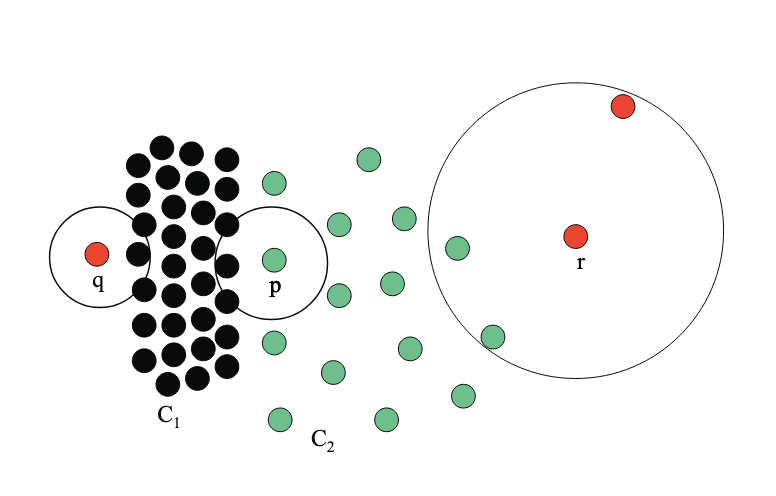
\includegraphics[width=0.5\linewidth]{img/inflo.png}
    \caption{In this example, points $q$ and $r$ have a lower LOF compared to $p$, despite it not being an outlier for the sparse cluster on the right.}
    \label{fig:inflo}
\end{figure}
The idea behind INFLO is to take symmetric neighborhood relationships into account. In other words, it considers both nearest neighbors as well as the reverse nearest neighbors (that is, the points having $p$ as a neighbor), defining the \textbf{influence space} of a point $p$ (indicated with $kIS(p)$).

Density is simply calculated as the inverse of the $k$-distance of a point. The INFLO is then calculated as:\begin{equation*}
    \textit{INFLO}_k(p) = \dfrac{\sum_{o \in kIS(p)} \dfrac{\textit{dens}(o)}{\# kIS(p)}}{dens(p)}
\end{equation*}
Similarly to LOF, if it is close to 1 the point is in a cluster, if instead it is much greater than 1, the point is an outlier.

\paragraph{Pros} Density-based approaches are, like distance based ones, very simple to implement.

\paragraph{Cons} They're computationally expensive since there is a need to find the distance between all points in the dataset, and densities are less meaningful as the dimensionality of the data increases. They are sensitive to the chosen hyperparameters.

\section{Clustering-based Approaches}

Cluster-based outliers are points that do not fit strongly into any cluster. For prototype-based clusters, it means they are far away from it; for density-based clusters, it means the object has a too low density around it; for graph-based clusters, it means the point in not well connected.

Some clustering algorithms are already capable of separating points belonging to clusters from outliers (DBSCAN, OPTICS). An idea would be to simply execute those algorithms feeding the dataset and choosing the appropriate hyperparameters, and analyze the set of ``noise'' points returned by them. However, these are first and foremost clustering algorithms: they are not optimized to find outliers and sets of abnormal data objects may be recognized as a cluster instead of outliers.

Just as we have seen for density-based outliers, we can use \textbf{Cluster-Based Local Outlier Factor} (\textbf{CBLOF}). To calculate it, first a clustering algorithm is used to find clusters in the dataset. Then, each cluster is classified as either a \textbf{small cluster} (\textbf{SC}), or \textbf{large cluster} (\textbf{LC}), using two parameters, $\alpha$ and $\beta$. Specifically, given the clustering $C = \{C_1, C_2, \dots, C_k \}$ such that $|C_1| \geq |C_2| \geq \dots \geq |C_k|$, a boundary $b$ is found if one of the following inequalities hold:
\begin{gather*}
    |C_1| + |C_2| + \dots + |C_b| \geq |D|*\alpha \\
    |C_b|/|C_{b+1} \geq \beta
\end{gather*}
This means that all clusters up until the $b^{th}$ contain $\alpha \%$ of the data points (first formula), or that the smallest of the large clusters must be at least $\beta$ times larger than the larger of the small clusters (second formula). 

The CBLOF is calculated depending on the size of the cluster the point belongs to, as well as the distance to the nearest large cluster. If the point is in a LC, the outlier score is the product between the size of the cluster and the distance with the cluster center. If it is in a SC, the score is the product between the size of the cluster and the distance to the center of the closest LC.
\begin{equation*}
    CBLOF(p) = \begin{cases}
        |C_i|*\min(d(p, C_j)), p \in C_i \land C_j \in LC & \text{if $C_i \in SC$} \\
        |C_i|*d(p, C_i) & \text{if $C_i \in LC$}
    \end{cases}
\end{equation*}

\paragraph{Pros} Cluster-based approaches are simple to implement and a variety of different algorithms exist.

\paragraph{Cons} A main issue is that the presence of outliers itself will distort the clustering. Also, it may be difficult choosing the appropriate hyperparameters and number of clusters when we don't have any knowledge about the structure of the data.

\section{High-dimensional Approaches}

All the approaches seen until now have one big problem in common: they are affected by the curse of dimensionality, and so they don't work well in high-dimensional spaces. An alternative to considering distances is instead considering angles, with \textbf{angle-based outlier detection}. The idea is to compare the angles between pairs of distance vectors that start from the same point. If a point is inside a cluster of data, most angles forming between distance vectors connecting that point and all other points will differ widely. For outliers, instead, all those angles will be similar to each other.
\begin{figure}[h]
    \centering
    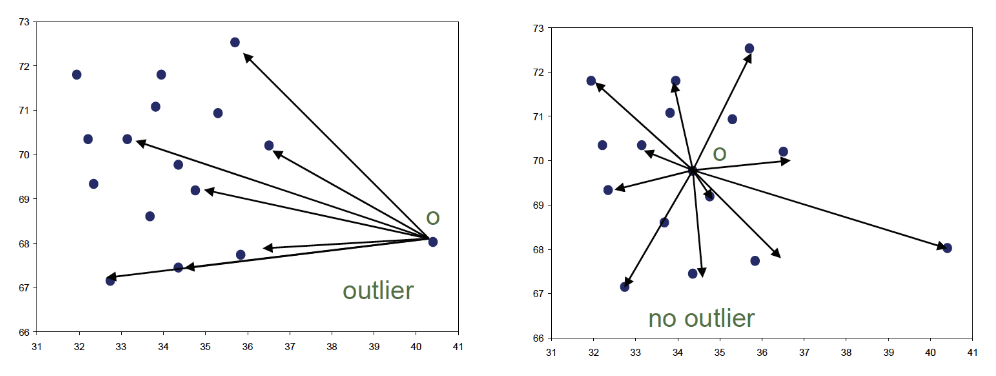
\includegraphics[width=0.7\linewidth]{img/angle_based_od.png}
    \caption{Intuition behind angle-based outlier detection.}
    \label{fig:angle-based}
\end{figure}
For each point $p$, the angle between any two other instances is calculated. The spectrum of all these angles is computed, and depending on its broadness, a score can be assigned to $p$: a small spectrum assigns an high outlier score, a large spectrum assign a small outlier score. Specifically, the \textbf{angle-based outlier degree} (\textbf{ABOD}) is assigned to $p$, calculated as the variance of the angle spectrum weighted by the corresponding distances:
\begin{equation*}
    \textit{ABOD}(p) = \underset{x,y \in D}{\mathrm{Var}} \left ( \dfrac{< \vec{xp}, \vec{yp} >}{\|\vec{xp}\|^2 \cdot \|\vec{yp}\|^2}  \right )
\end{equation*}
Note that the lower the ABOD, the more likely a point is to be an outlier.

The naive algorithm that calculates these degrees has a cost of $O(n^3)$, but it can be approximated by using random sampling to mine the top-$n$ outliers; ABOD is calculated only on the pairs of points in the sample, finding a lower bound of the real ABOD, and filtering out points that have a high ABOD lower bound. The real ABOD is only calculated for a small number of points.

A second approach is called \textbf{grid-based subspace outlier detection}. The data space of $k$ dimensions is partitioned into an equi-depth grid of $\Phi$ cells. The \textbf{sparsity coefficient} of a grid cell $C$ is:
\begin{equation*}
    S(C) = \dfrac{\textit{count}(C) - n (1/ \Phi)^k}{\sqrt{n(1/\Phi)^k (1-(1/\Phi)^k)}}
\end{equation*}
where $\textit{count}(C)$ is the number of data objects in $C$. If $S(C) < 0$, then $\textit{count}(C)$ is lower than expected: all points in those cells are labeled as outliers. This algorithm has a cost of $O(\Phi k)$.

This is a very coarse model: all the points within a cell with low sparsity are automatically outliers, without doing any further analysis on those points, so the quality of the result depends on the grid resolution and position. 

\section{Ensemble-based Approaches}

Ensemble-based means that a group of methods is used on the same dataset, and the final result will be a combination of their singular outcomes. For outlier detection, \textbf{feature bagging} (\textbf{FeaBag}) is used: a set of different outlier detection methods is selected, and each of them is applied on a random set of features selected from the original feature space. Each method will identify different outliers, assigning them outlier scores. The average of those scores is then returned for each point.

An extension of histogram-based outlier score is \textbf{lighteight on-line detector of anomalies} \textbf{(LODA)}. It is especially useful in real-time scenarios where a big amount of records must be processed. LODA approximates the joint probability using a collection of one-dimensional histograms, each constructed on an input space projected onto a randomly generated vector. Even thoug one-dimensional histograms are weak outlier detection methods by themselves, their collection yields good results.

\section{Model-based Approaches}

\textbf{Isolation forests} are a model specialized for outlier detection. First, a set of trees is initialized. Then, each tree receives a different sample of the data. The construction of the tree is done by repeating the following steps until the entire structure is complete, isolating each point in a leaf:
\begin{enumerate}
    \item Pick a random dimension;
    \item Pick a random value on that dimension;
    \item Draw a separating hyperplane at that value, and split the data in the two sides the hyperplanes separates them.
\end{enumerate}
Outliers will tend to be separated in few steps (so the leaves containing them will have low depth), while normal points will be separated after a long time (so they will be found in the deeper leaves). \\
Given a dataset of size $n$, the outlier score of a point $x$ is:
\begin{equation*}
    s(x,n) = 2^{\dfrac{-\mathrm{E}[h(x)]}{c(n)}}
\end{equation*}
where $h(x)$ represents the path length from the root to $x$, and $c(n)$ is the average $h(x)$ given $m$, calculated as:
\begin{equation*}
    c(m) = \begin{cases}
        1 & n = 2 \\
        2 * H(n-1) - \dfrac{2(n-1)}{n} & n > 2 \\
        0 & \text{else}
    \end{cases}
\end{equation*}
$H(i) = \ln(i) + \gamma, \gamma \approx 0.57$ is the $i^{th}$ \hyperlink{https://en.wikipedia.org/wiki/Harmonic_number}{harmonic number}.
\begin{figure}[h]
    \centering
    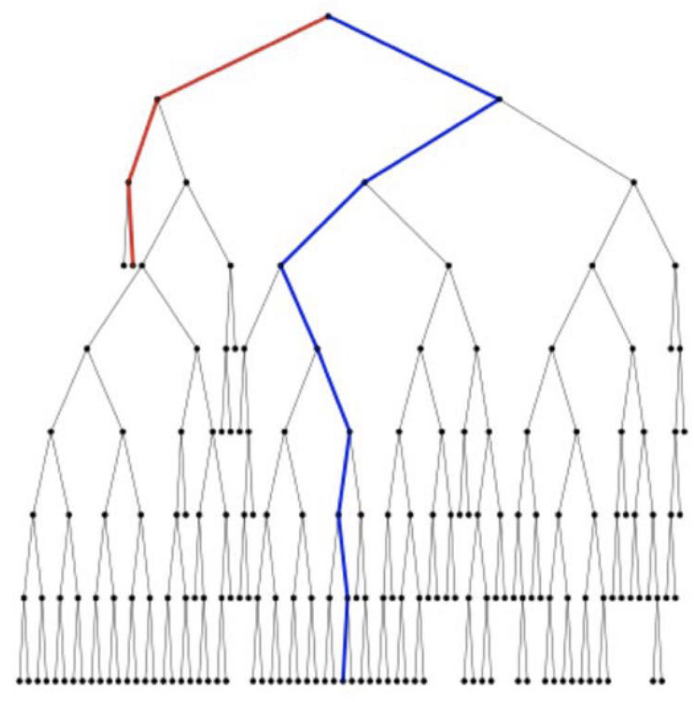
\includegraphics[width=0.35\linewidth]{img/isolation_tree.png}
    \caption{An example of tree: in red the path from the root to an anomaly, in blue the path to a normal point.}
    \label{fig:isolation-tree}
\end{figure}
Isolation forests are computationally efficient, paralellizable, and can handle high dimensional data. However, inconsistent scoring can be observed since the space is always split across one dimension at a time. The \textbf{extended isolation forest} model solves this problem: instead of choosing a dimension, each tree randomly selects both a normal vector and an intercept describing an angled hyperplane.
\clearpage
\begin{figure}[H]
    \centering
    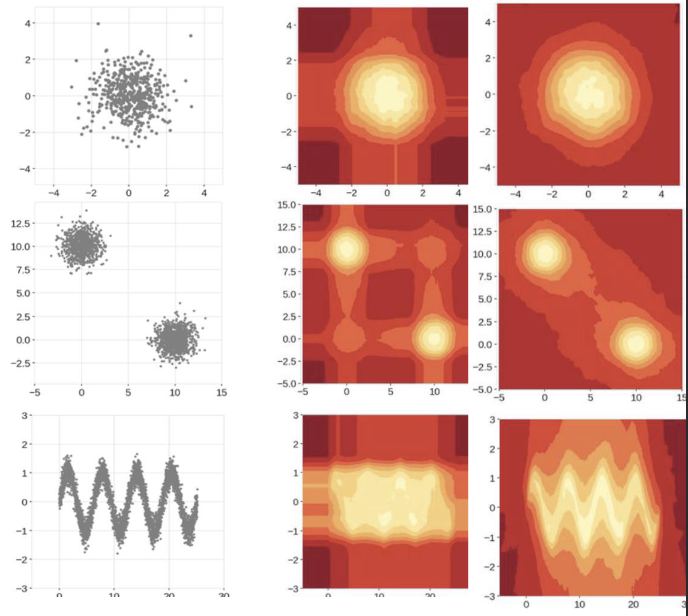
\includegraphics[width=0.5\linewidth]{img/isolation_forests.png}
    \caption{Isolation forests and Extended isolation forests, compared.}
    \label{fig:isolation-forests}
\end{figure}

\chapter{Logistic Regression}

Logistic regression is the task of finding a model that represents the log-odds of an event, used for binary classification problems. The function used by the model is called \textbf{logistic function}, which converts the log-odds of a point to the probability of it being labeled 0 or 1. The model is fitted to the data by maximum likelihood estimation.

The idea is to model the probability using a linear function, written as:
\begin{equation*}
    f(x_i) = \beta_1 x_i + \beta_0
\end{equation*}
where $\beta_0$ and $\beta_1$ are regression coefficients. Since the value returned by this function for each $x_i$ is its corresponding log-odds, we can write the following equation:
\begin{gather*}
    \ln \left (\dfrac{p}{1-p} \right ) = \beta_1 x_i + \beta_0 \\
    \iff \\
    \dfrac{p}{1-p} = e^{\beta_1 x_i + \beta_0} \\
    \iff \\
    p = e^{\beta_1 x_i + \beta_0} - p e^{\beta_1 x_i + \beta_0} \\
    \iff \\
    p + p e^{\beta_1 x_i + \beta_0} = e^{\beta_1 x_i + \beta_0} \\
    \iff \\
    p (1 + e^{\beta_1 x_i + \beta_0}) = e^{\beta_1 x_i + \beta_0} \\
    \iff \\
    \boxed{p = \dfrac{e^{\beta_1 x_i + \beta_0}}{1 + e^{\beta_1 x_i + \beta_0}} = \dfrac{1}{1 + e^{-(\beta_1 x_i + \beta_0)}}}
\end{gather*}
So, for a set of given values for the model's parameters, its \textbf{likelihood} is calculated as:
\begin{equation*}
    \mathcal{L}_n(\beta_0, \beta_1; x) = \prod_{i: y_i = 1} f(x_i) * \prod_{j: y_i = 0}^{l-k} 1 - f(x_j)
\end{equation*}
i.e., it's the product of the likelihoods of each data point. In practice, the \textbf{log-likelihood} is used instead:
\begin{equation*}
    l(\beta_0, \beta_1; x) = \sum_{i: y_i = 1} \ln(f(x_i)) + \sum_{j: y_j = 0} \ln(1 - f(x_i))
\end{equation*}
The likelihood is calculated for different parameters, gradually increasing it until it finds the optimal fit.
\chapter{Support Vector Machines}

Support Vector Machines (SVMs) are a type of model used for both classification and regression. They used to be the most popular approach for supervised learning when there's little to no domain knowledge for the data, but they've been mostly replaced by neural networks and random forests.

\section{Hard Margin SVM}

Assume a classification task. Given a training set $TR = <x_i,d_i>, \, i=1 \dots N$, we want to find an hyperplane of equation $w^T x + b = 0$ to separate the examples; specifically, we want:

\begin{gather*}
    w^T x_i + b \geq 0 \text{ for } d_i = +1 \\
    w^T x_i + b < 0 \text{ for } d_i = -1
\end{gather*}

$g(x) = w^T x + b$ is called the \textbf{discriminant function}, and $h(x) = sign(g(x))$ is the hypothesis. Note that here the bias is referred to as $b$ instead of $w_0$. To find the hyperplane that separates all the points, instead of simply minimizing the empirical risk, the SVM minimizes the expected generalization error by finding the separator that is farthest away from all the examples in the dataset. It also establishes a margin ($\rho$) around it, whose width is exactly twice the distance between the hyperplane and the closest data point(s). The optimal hyperplane is the one that maximizes this margin $\rho$: $w_o^Tx + b_o = 0$, where $\rho = 2 / \|w_o\|$.

The two terms $w$ and $b$ can be rescaled so that the closest points to the separating hyperplane satisfy $\|g(x)\| = 1$, so we can write:

\begin{gather*}
    w^T x_i + b \geq 1 \text{ for } d_i = +1 \\
    w^T x_i + b \leq -1 \text{ for } d_i = -1 \, ,
\end{gather*}
or, in a compact form,
\begin{gather*}
    d_i(w^T x_i + b) \geq 1 \, .
\end{gather*}
Any $x_i$ that satisfies this equation is called a \textbf{support vector}, and is referred to as $x^{(s)}$. Let's denote the distance between the optimal hyperplane and a point $x$ as $r$, such that $x = x_p + r\frac{w_o}{\|w_o\|}$ (where $x_p$ is a point on the hyperplane). Evaluating $g(x)$ we obtain:

\begin{align*}
    g(x) = g(x_p + r\dfrac{w_o}{\|w_o\|}) = \\
    = w_o^Tx_p + b_o + w_o^T r \dfrac{w_o}{\|w_o\|} = \\
    = g(x_p) + w_o^T r \dfrac{w_o}{\|w_o\|} = \\
    = 0 + r \dfrac{\|w_o\|^2}{\|w_o\|} = r \|w_o\| \, ,
\end{align*}
thus, $r = \dfrac{g(x)}{\|w_o\|}$. \\
Consider the distance between the hyperplane and a positive support vector $x^{(s)}$, then $r$ is calculated as:

\begin{equation*}
    r = \dfrac{g(x^{(s)})}{\|w_o\|} = \dfrac{1}{\|w_o\|} = \dfrac{\rho}{2} \, ,
\end{equation*}
therefore, $\rho = \dfrac{2}{\|w_o\|}$.

\subsection{Primal Problem}

The optimum hyperplane will maximize $\rho$ and minimize $\|w\|$. One approach to find it is to perform a gradient descent to find the $w$ and $b$ that minimize/maximizes them, but there's another approach, that is solving a \textbf{quadratic optimization problem}.

\BoxDef{Quadratic optimization problem (primal form)}{
Given the training examples $TR = < x_i,d_i >$, find the optimal values of $w$ and $b$ which minimize
\begin{equation*}
    \Psi (w) = \dfrac{1}{2}w^T w
\end{equation*}
satisfying the constraints
\begin{equation*}
    d_i(w^T x_i + b) \geq 1 \, .
\end{equation*}
}
The objective function $\Psi (w)$ is quadratic and convex in $w$. The constraints are linear in $w$, and solving the problem scales with the size of the input space $m$.

To solve this problem, the \textbf{Lagrangian multipliers method} is used. The Lagrangian function corresponding to the quadratic optimization problem is constructed:
\begin{equation*}
    J(w,b,\alpha) = \dfrac{1}{2}w^T w - \sum_{i=1}^N \alpha_i(d_i(w^T x_i + b) - 1) \, ,
\end{equation*}
where $\alpha_i \geq 0$ are the \textbf{Lagrangian multipliers}. Each term in the sum corresponds to a constraint of the primal problem; $J$ must be minimized with respect to $w$ and $b$ and maximized with respect to $\alpha$. The solution will correspond to a saddle point of $J$. \\
If we minimize $J$ with respect to $w$, then:
\begin{gather*}
    \dfrac{\partial J}{\partial w} = \dfrac{2}{2} w - \sum_{i=1}^N \alpha_i(d_i(1*x_i + 0) + 0) = \\
    = w - \sum_{i=1}^N \alpha_i(d_i(x_i)) = 0
\end{gather*}
so
\begin{equation*}
    w = \sum_{i=1}^N \alpha_i(d_i(x_i)) \, .
\end{equation*}
Thus the optimal hyperplane is expressed as:
\begin{gather*}
    g(x) = w_o^T x + b_o = 0 \\
    \iff \\
    \sum_{i=1}^N \alpha_{o,i} d_i x_i^T x + b_o = 0 \, .
\end{gather*}
If instead we minimize it with respect to $b$:
\begin{gather*}
    \dfrac{\partial J}{\partial b} = 0 - \sum_{i=1}^N \alpha_i d_i = 0 \, .
\end{gather*}
These can be substituted in $J$ to study the dual form of the problem. \\
From the \textbf{Kuhn-Tucker Conditions}, it follows that
\begin{equation*}
    \alpha_i (d_i (w^T x_i + b) - 1) = 0 \, , \forall i = 1, \dots , N
\end{equation*}
in the saddle point of $J$. If $\alpha_i > 0$, then $(d_i (w^T x_i + b) = 1$, and $x_i$ is a support vector. If $x_i$ is not a support vector, then $\alpha_i = 0$. Hence we can restrict the computation to $N_s : w_o = \sum_{i=1}^{N_s} \alpha_{o,i} d_i x_i$. The hyperplane depends only on support vectors.

\subsection{Dual Problem}

To obtain the Lagrangian multipliers $\alpha_i$, we solve the problem in its dual form:

\BoxDef{Quadratic optimization problem (dual form)}{
Given the training examples $TR = < x_i,d_i >$, find the optimal values of $\alpha_i$ which maximize
\begin{equation*}
    Q(\alpha) = \sum_{i=1}^N \alpha_i - \dfrac{1}{2} \sum_{i=1}^N \sum_{j=1}^N \alpha_i \alpha_j d_i d_j x_i^T x_j
\end{equation*}
satisfying the constraints
\begin{gather*}
    \alpha_i \geq 0 \, , \forall i = 1, \dots , N \, ,\\
    \sum_{i=1}^N \alpha_i d_i = 0 \, .
\end{gather*}
}
The value of $\alpha_i$ can be found by solving the quadratic programming (QP) problem, or by more recent and efficient approaches (such as sequential minimal optimization (SMO)). Solving this problem scales with the number of training examples, less with the dimensionality. To find $w_o$ and $b_o$, we proceed as follows:
\begin{gather*}
    w_o = \sum_{i=1}^N \alpha_{o,i} d_i x_i \\
    b_o = 1 - w_o^T x^{(s)} = 1 - \sum_{i=1}^N \alpha_{o,i} d_i x_i^T x^{(s)} \, .
\end{gather*}
How do we use all of this? We don't actually need to explicitly know $w_o$. All we need are calculating the Lagrangian multipliers by solving the dual problem, and then calculating $b_o$. So, given the input pattern $x$, we compute $g(x) = \sum_{i=1}^N \alpha_{o,i} d_i x_i^T x + b_o$, and classify it as $h(x) = sign(g(x))$.

This approach of finding optimal separating hyperplane maximizing the margin also provides:
\begin{itemize}
    \item An unique solution with zero errors for the binary classifier;
    \item An automatized approach to Structural Risk Minimization that minimizes the VC-confidence without having to deal with hyperparameters;
    \item The use of a solver in the class of constrained quadratic programming (instead of gradient descent) with a nice dual form;
    \item A solution focused on a selection of training data points: the support vectors.
\end{itemize}
But what about noisy or non linearly separable data?

\section{Soft Margin SVM}

In realistic datasets, the training set is not going to be perfect. It will contain noisy points and outliers that make the problem not linearly separable. The solution is to find a separator with a soft margin, that is, a margin that allows some errors within it. Because the margin can allow points to fall inside of it, the support vectors are no longer going to be the closest points to the margin.

We introduce what are called \textbf{slack variables}, which are non negative scalar variables:

\begin{gather*}
    \xi_i \geq 0 \, , \forall i = 1, \dots , N \\
    d_i(w^T x_i + b) \geq 1 - \xi_i \, , \forall i = 1, \dots , N
\end{gather*}
If $x^{(s)}$ is a support vector, it will satisfy the equation:
\begin{equation*}
    d_i(w^T x^{(s)} + b) = 1 - \xi_i 
\end{equation*}
The problem can be then rewritten to admit points in the margin.

\BoxDef{Quadratic optimization problem with Soft Margin (primal form)}{
Given the training examples $TR = < x_i,d_i >$, find the optimal values of $w$ and $b$ which minimize
\begin{equation*}
    \Psi(w, \xi) = \dfrac{1}{2}w^T w + C \sum_{i=1}^N \xi_i
\end{equation*}
satisfying the constraints
\begin{gather*}
    d_i (w^T x_i + b) \geq 1 - \xi_i \, , \forall i = 1, \dots N \\
    \xi_i \geq 0 \,, \forall i = 1, \dots N
\end{gather*}
}
The term $C$ is a user-defined regularization hyperparameter; so this version of SVM is no longer ``automatic'' like hard margin SVM was. $C$ is found as the trade-off between empirical risk minimization and capacity term (VC-confidence). If $C$ is too low, we allow many training errors, leading to underfitting. If $C$ is too high, we don't let any training error, leading to overfitting.

\BoxDef{Quadratic optimization problem with Soft Margin (dual form)}{
Given the training examples $TR = < x_i,d_i >$, find the optimal values of $\alpha_i$ which maximize
\begin{equation*}
    Q(\alpha) = \sum_{i=1}^N \alpha_i - \dfrac{1}{2}\sum_{i=1}^N \sum_{j=1}^N \alpha_i \alpha_j d_i d_j x_i^T x_j
\end{equation*}
satisfying the constraints
\begin{gather*}
    0 \leq \alpha_i \leq C \, , \forall i = 1, \dots , N \\
    \sum_{i=1}^N \alpha_i d_i = 0
\end{gather*}
}
The Kuhn-Tucker conditions can be redefined as:
\begin{gather*}
    \alpha_i (d_i (w^T x_i + b) + \xi_i - 1) = 0 \, , \forall i = 1, \dots , N \\
    \mu_i \xi_i = 0 \,, \forall i = 1, \dots , N \, ,
\end{gather*}
where $\mu_i$ are Lagrange multipliers introduced to enforce non-negativity of the slack variables in the primal function. If $0 < \alpha_i < C$, then $\xi_i = 0$. If $\alpha = C$, then $\xi_i \geq 0$. To solve the problem, we again solve the dual problem with respect to $\alpha_i$, and calculate $w_o$ and $b_o$ exactly as before.

\section{Mapping To a High-dimensional Space}

\href{https://en.wikipedia.org/wiki/Cover%27s_theorem#The_Theorem}{If the TR set represents a non-linearly separable problem, the data points can be mapped from the input space to a high-dimensional \textbf{feature space}, where they are linearly separable}. The approach we follow is analogous to the LBE for linear models. We define some function $\phi : \mathbb{R}^{m_0}\xrightarrow{} \mathbb{R}^{m_1}$. Finding this function, however, is not always easy, unless we have some prior knowledge allowing us to select the proper feature space. Also, using high dimensional feature spaces can lead to overfitting.

Given this function, we map all points to the new feature space: $x \mapsto \phi(x)$. The problem is formulated as before, with a new training set $TR = < \phi(x_i),d_i >$, and a new hyperplane $g(x) = w^T \phi(x) + b = 0$. The notation used here incorporates the bias in the weight vector, with $w_0 = b$ and $\phi_0(x) = 1$:
\begin{equation*}
    \phi(x) = (\phi_0(x) = 1, \phi_1(x), \dots , \phi_{m_1}(x))^T
\end{equation*}
The weight vector is now a linear combination of the feature vectors:
\begin{equation*}
    w = \sum_{i=1}^N \alpha_i d_i \phi(x_i)
\end{equation*}
and the hyperplane equation can be written as:
\begin{equation*}
    g(x) = \sum_{i=1}^N \alpha_i d_i \phi^T (x_i) \phi(x) = 0
\end{equation*}
Evaluating $\phi(x)$ may be intractable. Fortunately, under certain conditions we do not need to evaluate it directly, or even know the feature space itself. This is possible with a so-called \textbf{kernel trick}, i.e. by using a function $k$ to directly compute the dot products $\phi^T (x_i) \phi(x)$ in the feature space:
\begin{equation*}
    k : \mathbb{R}^{m_0} \times \mathbb{R}^{m_0} \xrightarrow{} \mathbb{R}
\end{equation*}
This function is known as the \textbf{inner product kernel function}. It's also a symmetric function, so $k(x_i, x) = k(x, x_i)$. Consider the function $\phi(x) = \phi((x_1, x_2)^T) = (x_1^2, \sqrt{2}x_1x_2, x_2^2)^T$. Given $x = (x_1, x_2)^T$ and $y=(y_1,y_2)^T$ in $\mathbb{R}^2$, we compute $\phi^T(x)\phi(y)$ in this 
\begin{gather*}
    \phi^T(x)\phi(y) = (x_1^2, \sqrt{2}x_1x_2, x_2^2) (y_1^2, \sqrt{2}y_1x_2, y_2^2)^T = \\
    x_1^2y_1^2 + 2x_1y_1x_2y_2 + x_2^2y_2^2 = (x_1y_1 + x_2y_2)^2 = \\
    ((x_1,x_2)(y_1,y_2)^T)^2 = (x^Ty)^2 = k(x,y)
\end{gather*}
We can arrange the dot products in the feature space between the image of the input training patterns in a $N$ by $N$ matrix, called \textbf{kernel matrix}:
\begin{equation*}
    K = \begin{pmatrix}
        k(x_1,x_1) & \dots & k(x_1, x_N) \\
        k(x_2,x_1) & \dots & k(x_2, x_N) \\
        \vdots & & \vdots \\
        k(x_N,x_1) & \dots & k(x_N, x_N) \\
        \end{pmatrix} \,, \,
        K = \{k(x_i, x_j)\}_{(i,j)=1)}^N
\end{equation*}
The kernel matrix is symmetrical, as the inner product kernel is symmetrical. Not every kernel function computes the inner product in a feature space; \href{https://en.wikipedia.org/wiki/Mercer%27s_theorem}{this property holds only for kernels gaining positive semi-definite kernel matrices. This is related to the matrix having non negative Eigenvalues}. \\
Given $k_1$ and $k_2$ both kernels over $\mathbb{R}^{m_0} \times \mathbb{R}^{m_0}$. The following are also kernel functions:
\begin{itemize}
    \item $k_1(x,y) + k_2(x,y)$;
    \item $\alpha k_1(x,y) \, \forall \alpha \in \mathbb{R}_+$;
    \item $k_1(x,y)k_2(x,y)$.
\end{itemize}
The problem is reformulated in both forms as follows.

\BoxDef{Quadratic optimization problem in feature space (primal form)}{
Given the training examples $TR = < \phi(x_i),d_i >$, find the optimal values of $w$ which minimizes
\begin{equation*}
    \Psi(w, \xi) = \dfrac{1}{2}w^T w + C \sum_{i=1}^N \xi_i
\end{equation*}
satisfying the constraints
\begin{gather*}
    d_i (w^T \phi(x_i)) \geq 1 - \xi_i \, , \forall i = 1, \dots N \\
    \xi_i \geq 0 \,, \forall i = 1, \dots N
\end{gather*}
}

\BoxDef{Quadratic optimization problem in feature space (dual form)}{
Given the training examples $TR = < \phi(x_i),d_i >$, find the optimal values of $\alpha_i$ which maximize
\begin{equation*}
    Q(\alpha) = \sum_{i=1}^N \alpha_i - \dfrac{1}{2}\sum_{i,j=1}^N \alpha_i \alpha_j d_i d_j k(x_i,x_j)
\end{equation*}
satisfying the constraints
\begin{gather*}
    \sum_{i=1}^N \alpha_i d_i = 0 \\
    0 \leq \alpha_i \leq C \,, \forall i = 1, \dots N
\end{gather*}
}
To classify an unseen input pattern $x$ using the machine we trained, we compute $\sum_i \alpha_i d_i k(x, x_i)$, and then classify $x$ as $h(x) = sign(\sum_{i=1}^n \alpha_i d_i k(x, x_i))$. Note: we have to memorize the $x_i$ in the training set for the test phase.

Some examples of commonly used kernels include:
\begin{itemize}
    \item \textbf{Polynomial Learning Machine}: $k(x,x_i) = (x^T x_i + 1)^p$ (where $p$ is a user-specified parameter);
    \item \textbf{Radial Basis Function Net}: $k(x, x_i) = e^{-\frac{\|x - x_i\|^2}{2 \sigma^2}}$ (where $\sigma$ is a user-specified parameter);
    \item \textbf{Two-layer Perceptron}: $k(x,x_i) = tanh(\beta_0 x^T x_i + \beta_1)$ (where $\beta_0 > 0$ and $\beta_1 < 0$ are user-specified parameters).
\end{itemize}
Using an RBF always leads to a feature space with an infinite number of dimensions.

\section{Pros and Cons of SVM}

\textbf{Pros:}
\begin{itemize}
    \item The regularization is embedded within the optimization problem, so it does not need any external hyperparameter for it;
    \item It automatically approximates SRM by finding the hypothesis with the best possible VC-dim;
    \item It's a convex problem, so the global minimum can always be found;
    \item Features are implicitly transformed through kernels;
    \item Linear model with bound of the  complexity that depends on the margin (which is optimized);
    \item Rich set of non-linear decision functions in the input space via kernels.
\end{itemize}

\textbf{Cons:}
\begin{itemize}
    \item Kernel and kernel parameters must be chosen explicitly;
    \item It uses a batch algorithm to update the weights, so no chance to parallelize;
    \item Very large problems were computationally intractable (although nowadays many efficient solutions have been proposed, including gradient descent ones);
    \item For soft margin SVM, since we have to select the $C$ parameter and the kernel function, we have no guarantee that the final model will have high accuracy.
\end{itemize}

Note that for the last point about soft margin, the VC-dim of the model is controlled by the width of the margin. If we choose the smallest possible margin (with just one support vector), we can classify an arbitrarily large number of training points correctly, thus the VC-dim will be infinite. If instead we have a very large width, we end up in a situation where all points in the TR set are used as support vectors, therefore leading to a low VC-dim. This is analogous to using a k-NN classifier with $k=1$ and $k=l$, respectively. Also, the hyperparameter $C$ used for regularization must be chosen appropriately for the kernel hyperparameters, so cross-validation is needed.

\chapter{Neural Networks}

(Artificial) neural networks are a flexible machine learning tool, encompassing a wide set of models capable of approximating functions. They can learn from examples, are universal approximators (\href{https://en.wikipedia.org/wiki/Universal_approximation_theorem}{Cybenko's/Universal approximation Theorem}), can deal with noisy and/or incomplete data, and can handle both continuous real and discrete data.

\section{Artificial Neurons}

Artificial neural networks are made up of several \textbf{nodes} (also called artificial neurons, or units) connected in a net capable of solving artificial intelligence problems. They are heavily inspired by biological neural networks, down to how the single units work and communicate with each other to learn a certain function. \\
The main ideas that these models are based on are:

\begin{itemize}
    \item \textbf{Strength reinforcement}: stimuli ``reinforce'' the weights;

    \item \textbf{Plasticity}: the nervous system is highly capable of adapting.
\end{itemize}

Each neuron $i$ has a number of \textbf{inputs} coming from external sources or other units, and corresponding \textbf{weights}, the free parameters that can be modified during the learning phase. Each neuron calculates its \textbf{net input} (weighted sum of inputs) and its output as follows:

\begin{equation*}
    \begin{cases}
        net_i(x) = \sum_j w_{ij} x_j \\
        o_i(x) = f(net_i(x)),
    \end{cases}
\end{equation*}
where $f$ is the unit's \textbf{activator function}. Note that $w_{ij}$ is the weight of the input coming from the node $j$ and going into the node $i$; some books/libraries/simulators, etc. may use the opposite notation.

\begin{figure}[ht]
    \centering
    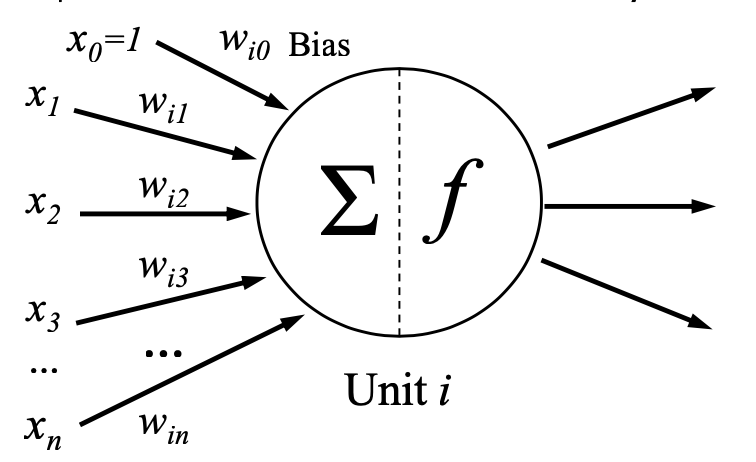
\includegraphics[width=0.5\linewidth]{img/Neuron.png}
\end{figure}

\subsection{Perceptrons}

The perceptron was proposed and implemented in 1958 by Frank Rosenblatt. The first perceptron was an actual physical machine designed for image recognition, and not a program. It had a few hundreds of photocells, randomly connected to a layer of neurons. Multiple perceptrons can be composed and connected to build a network. This is called a \textbf{multi-layer perceptron neural network (MLP NN)}. 

McCulloch and Pitts proposed a neural network model in 1943. In this model, each neuron is in one of two possible states: firing (1), or not firing (0). All synapses (connections) are equivalent and characterized by a weight $w_i$ which is positive for ``excitatory'' connections, and negative for ``inhibitory'' connections. A neuron $i$ becomes active when the sum of the connections coming from other active neurons and the bias is larger than 0. Both inputs and outputs are binary, so it can implement binary classification tasks.

The following pictures illustrate how this model can be used to represent boolean functions AND and OR by using a single neuron. Each neuron has two inputs, plus a bias ($w_0$). Both problems are linearly separable, so if the inputs are represented graphically on a plane, we can draw a single line (described by the net function) that separates all inputs that produce a 0 from all the ones that produce a 1.

\begin{figure}[ht]
    \centering
    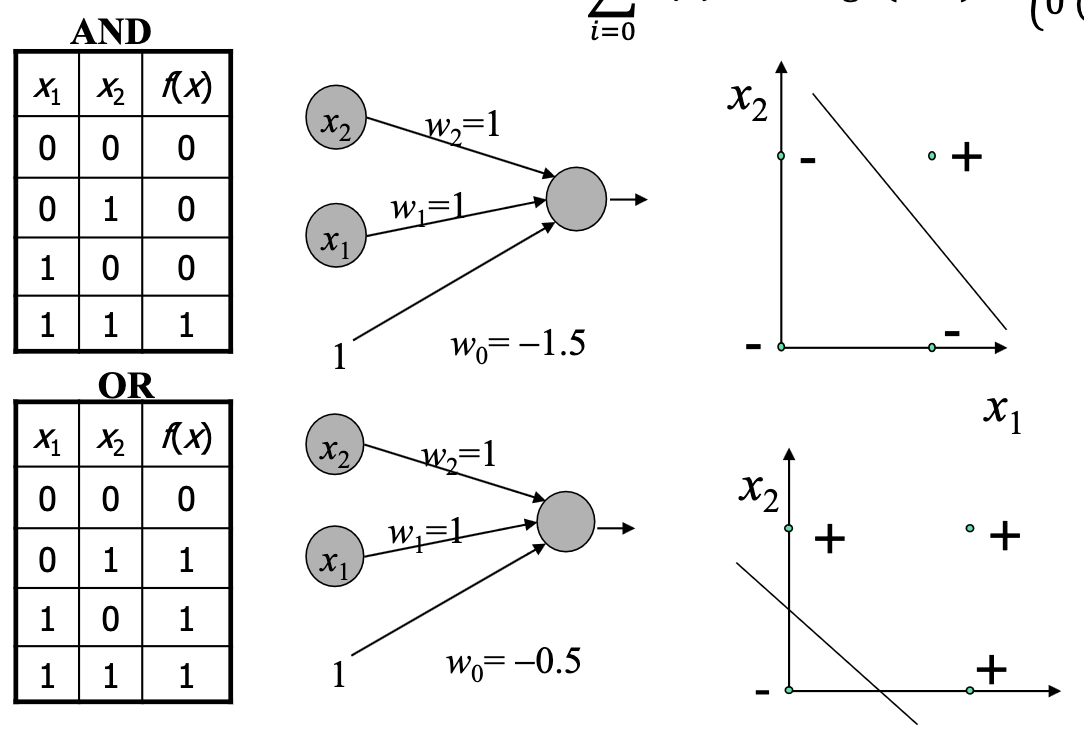
\includegraphics[width=0.5\linewidth]{img/boolean perceptron.png}
\end{figure}

If we instead consider the XOR operator, it corresponds to a non-linearly separable problem, so we can't use a single neuron. The solution is to use a two layer network. The operation can be rewritten as follows:

\begin{equation*}
    x_1 \oplus x_2 = x_1 \cdot \Bar{x_2} + \Bar{x_1} \cdot x_2
\end{equation*}
then we have:
\begin{equation*}
    x_1 \oplus x_2 = \Bar{h_1} \cdot h_2
\end{equation*}
So the XOR operation is moved to a new space that represents the problem as linearly separable:
\begin{figure}[ht]
    \centering
    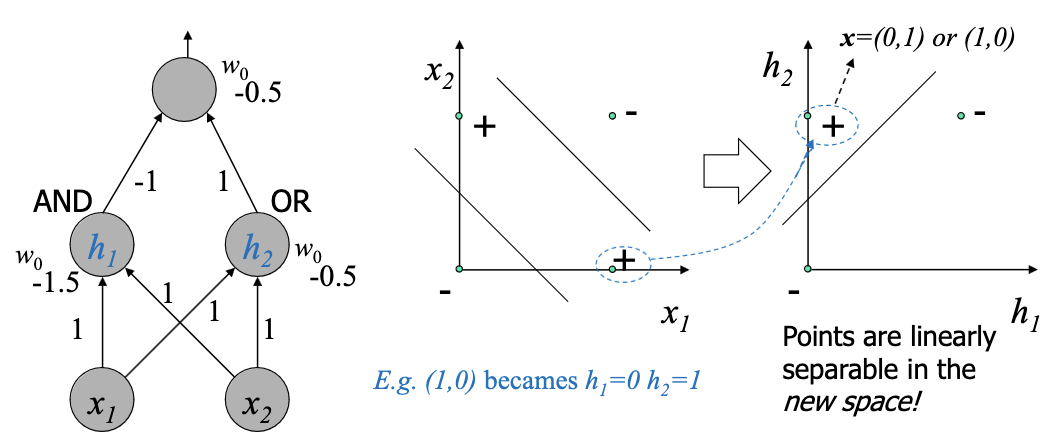
\includegraphics[width=0.55\linewidth]{img/xor perceptron.png}
\end{figure}
This type of composition can be used to perform more complex tasks, extending the network to many layers of abstraction. In NN, this internal representation can be learned.

\section{Learning Algorithms For One Unit Models}

There's two kinds of learning algorithms:
\begin{itemize}
    \item \textbf{Adaline (Adaptive Linear Neuron)}: linear unit during training, can use LMS with either SVD or gradient descent algorithm. This approach an be generalized to multi-level perceptron NNs.

    \item \textbf{Perceptron}: non-linear unit during training, with hard limit or threshold activation function. Can only be used for classification.
\end{itemize}

\subsection{Perceptron Learning Algorithm}

The goal of the algorithm is to minimize the number of misclassified patterns; so it must find $w$ such that $sign(w^Tx)=d$. This is an on-line algorithm, so one step can be done for each input pattern. The algorithm can be summarized as follows:

\begin{enumerate}
    \item Initialize the weights (either to 0 or a small random value);

    \item Pick a learning rate $\eta$;

    \item For each training pattern $<x,d>$, where $d$ is either $+1$ or $-1$, compute $out = sign(w^Tx)$; if $out = d$, don't change the weights, otherwise modify the weights as:
    \begin{equation*}
        w_{new} = w + \eta d x
    \end{equation*}
    or, in a different form,
    \begin{equation*}
        w_{new} = w + \frac{1}{2} \eta (d-out) x
    \end{equation*}
\end{enumerate}

Looking at the problem from a geometrical point of view, it's as if we modified the weight vector $w$ by summing the vector $\eta d x$, where $d$ indicates the direction of the vector with respect to that $x$: if positive, the addition will move $w$ ``towards'' the point, if negative, it will move it ``away'' from it. \\
The form $w_{new} = w + \eta d x$ is in the form of Hebbian learning, while $w_{new} = w + \eta (d-out) x = w + \eta \delta x$ is in the form of error-correcting learning.

\subsection{Differences Between LMS and Perceptron Learning Algorithm}

They are apparently very similar; they both calculate the new value of $w$ by adding a $\delta$ multiplied by the learning rate $\eta$, along with the input $x$ for the Perceptron Learning Algorithm. The $\delta$ for LMS is calculated as $(d - w^Tx)$, while for perceptron learning algorithm it's $(d - sign(w^Tx))$. However similar they are, there a few important differences:

\begin{itemize}
    \item LMS does not necessarily minimize the number of training examples misclassified by the LTU, since it changes the weights for both misclassified and correctly classified ones;

    \item The perceptron learning algorithm always converges for a linear separable problem to a perfect classifier, while LMS has asymptotic convergence (also for non linearly separable problems);

    \item The perceptron learning algorithm is difficult to extend to a NN, while the LMS can be extended to a NN by using the gradient based approach.
\end{itemize}

\section{Activation Functions}

As seen before, the possible activation functions can be a linear function, a threshold function (perceptron/LTU), or a non-linear function such as the \textbf{sigmoidal logistic function}. The latter is a function that assumes a continuous range of values in the bounded interval $[0,1]$. It has the important property of being a smoothed differentiable function. The slope of the sigmoid function is defined by the parameter $a$. Some common examples of functions are:

\begin{itemize}
    \item \textbf{Logistic function}: $f_{\sigma}(x) = \dfrac{1}{1+e^{-ax}}$ (with output in the range $[0,1]$)

    \item \textbf{tanh function}: $f_{tanh}(\frac{x}{2}) = 2f_{\sigma}(x) - 1$ (with output in the range $[-1,+1]$)

    \item \textbf{Radial basis function}: $f(x) = e^{-ax^2}$

    \item \textbf{Rectified linear unit (ReLU)}:
    $f(x) = \begin{cases}
            0 & x < 0 \\
            x & x \geq 0
            \end{cases}$

    \item \textbf{Softplus function}: $f(x) = ln(1+e^x)$
\end{itemize}
The derivative of the identity function is 1. The derivative of the threshold function is not defined, which is why it's not used in LMS. As for sigmoid functions:

\begin{equation*}
    \dfrac{df_{\sigma}(x)}{dx} = f_{\sigma}(x)(1-f_{\sigma}(x)) 
\end{equation*}

\begin{equation*}
    \dfrac{df_{tanh}(x)}{dx} = 1 - f_{tanh}(x)^2
\end{equation*}

\section{LMS With Sigmoidal Function}

Since the sigmoidal logistic function is differentiable, we can derive a LMS algorithm by computing the gradient of the mean square loss function as for the linear units. The output of a neuron is calculated as:
\begin{equation*}
    out(x) = f_{\sigma}(x^Tw)
\end{equation*}
The objective of the algorithm is to find $w = argmin_w E(w) = \sum_p (d_p - out(x_p))^2 = \sum_p (d_p - f_{\sigma}(x_p^Tw))^2$, so the weights that minimize the residual sum of squares.

The gradient descent algorithm is the same, except it uses the new delta rule: $w_{new} = w + \eta \delta_p x_p$, where $\delta_p = (d_p - out(x_p))f'_{\sigma}$. Additionally, the parameter $a$, the slope of the function $f_{\sigma}$, can affect the step of the gradient descent.

Overall: the max of $f'$ corresponds to net inputs close to 0, while the minimum of $f'$ corresponds to \textbf{saturated cases}, as in where the function $f$ goes to either 0 or 1 asymptotically.

\section{Multi Layer Perceptrons}

A MLP can be seen in two possible ways: either as a network of units, or as a flexible function. As a network, a MLP contains a number of units connected by \textbf{weighted links}. The units are organized in layers: the first layer that loads the input is called the \textbf{input layer}; the layer that produces the final output is called the \textbf{output layer}; all other inbetween layers are called \textbf{hidden layers}. The notation used to refer to networks will be the following:

\begin{itemize}
    \item the index $t$ denotes a generic unit, while $k$ denotes an output unit;

    \item the index $u$ denotes a generic input component;

    \item $x$ is a generic input from an external source (if it's an input vector) or from another unit;

    \item if the pattern $x$ is loaded in the input layer, the notation $o$ can be used for both inputs and hidden layer inputs, so, inside the network, the input to each unit $t$ from any source $u$ is simply denoted as $o_u$.
\end{itemize}
As a flexible function, the MLP can be written as a function in the following form:

\begin{equation*}
    h(x) = f_k(\sum_j w_{kj} f_j (\sum_i w_{ji} f_i(\dots))) \, ,
\end{equation*}
where $f_k$ is a sigmoid activation function.

\subsection{Architecture}

The architecture of a NN defines the topology of the connections between units. A \textbf{feedforward architecture} describes a network that operates as follows. For each input pattern $x$, do:

\begin{enumerate}
    \item load the input in the input layer;
    \item compute the output of all the units in the first hidden layer;
    \item compute the output of all the units in the second hidden layer;
    \item ...
    \item compute the output of all the units in the output layer;
    \item compute the error (delta) at the output level.
\end{enumerate}
A \textbf{recurrent architecture} describes a network with feedback loops, which allow the output of units to go ``back'' in the network towards units in previous layers.

\section{Flexibility of NNs}

The hypothesis space of a NN is the continuous space of all the functions that can be represented by assigning the weight values of the given architecture. Depending on the class of values produced as output, the model can deal with both regression and classification tasks, by using, respectively, a linear function or a sigmoidal one. It can also implement multi-regression and multi-class classifiers by defining multiple output units. \\
When we consider a NN as a function, so in the form
\begin{equation*}
    h(x) = f_k(\sum_j w_{kj} f_j (\sum_i w_{ji} f_i(\dots))) \, ,
\end{equation*}
each $f_j$ can be seen as computed by an independent unit, or a special kind of $\phi$ of Linear Basis Expansion. Additionally, $h(x)$ is non-linear in the parameters $w$. So, we can reformulate the function as follows:
\begin{equation*}
    h(x) = f_k(\sum_j w_{kj} f_j (\sum_i w_{ji} x_i)) = f(\sum_j w_j \phi_j(x,w))
\end{equation*}
The main difference with LBE is that the $\phi$ are adapted to data by fitting the $w$.

\subsection{Theoretical Grounds}

The universal approximation theorem declares that single hidden-layer network (with logistic activation functions) can approximate (arbitrarily well) every continuous function, given enough units; a MLP network can approximate (arbitrarily well) every input-output mapping (provided enough units in the hidden layers), as well. Note that this theorem does not say which learning algorithm to use, nor the number of units needed.

Two issues arise: how can we learn with a NN?, and, how can we decide what NN architecture to use? The answers to these two questions will be provided later. The expressive power of NN is strongly influenced by two aspects: the number of units and the architecture. More specifically, the number of parameters $w$ (which is proportional to the number of units) influences the network capabilities; additionally, even their value can influence the VC-dim of the network: the lower the weights, the lower the VC-dim.

Another important aspect is the number of layers to use in the network. The universal approximation theorem tells us that 1 layer is sufficient to approximate any function, yet it gives no indication on the number of units to use, which may be incredibly high. So, instead of using only one layer, the network is split into multiple layers, each with a limited number of units.

\section{Backpropagation Learning Algorithm}

The learning algorithm used for NN follows the LMS approach. The goal is to adapt the free parameters $w$ in order to obtain the best approximation of the target function. This is normally done by checking the value of the error (or loss) function calculated on the training set. In the case of NNs, however, this is not as straightforward: the network has multiple units across layers, so the learning algorithm must first decide how much credit to give to the hidden units in causing the error to increase.

The so called \textbf{loading problem} is formulated as follows: given a network and a set of examples, is there a set of weights so that the network will be consistent with the examples? The problem is NP-complete, and while networks can in practice be trained in a reasonable amount of time, an optimal solution in not guaranteed.

The idea behind the backpropagation algorithm solution is to extend the gradient descent approach, so it can be used with MLP networks as well. The things we need are:
\begin{itemize}
    \item differentiable loss;
    \item differentiable activation functions;
    \item a network to follow the information flow.
\end{itemize}
What we want to find is $w$ obtained by computing the gradient of the error function. The advantages of the backpropagation algorithm are:
\begin{itemize}
    \item it's easy because of the compositional form of the model;
    \item it keeps track of the quantities local to each unit;
    \item it's efficient, since it's $O(\#W)$ rather than $O(\#W^2)$
    \item supposedly, the brain's learning ``algorithm'' is a local sub optimal approximation of backpropagation (although this debate remains controversial).
\end{itemize}

\subsection{Issues in Training NNs}

The resulting model is often over-parameterized; additionally, the optimization problem is no longer convex, and is potentially unstable.

Some problems in training NNs involve:
\begin{itemize}
    \item \textbf{Hyperparameters}: starting values, choosing between on-line/batch, learning rate, number of hidden units in the network;

    \item \textbf{Multiple minima}: the loss is no longer a simple convex function, so finding a minimum needs specific techniques;

    \item \textbf{Stopping criteria};

    \item \textbf{Overfitting and regularization};

    \item \textbf{Input scaling/output representation}.
\end{itemize}

\subsubsection{Hyperparameters}

\paragraph{Starting values}

The weights are normally initialized with random values near 0; we want to avoid a completely null weight vector, too high values, or all components equal to each other, since these can hamper training. We can also consider the \textbf{fan-in}, i.e., the number of inputs to a hidden unit: $range * 2 /fan-in$. This should be avoided if the fan-in is too large, or if the unit in question is an output unit, since the $\delta$ would be too close to 0 (since we're using backpropagation, those $\delta$ values would be propagated to previous layers, and cause all others to decrease as well).

\paragraph{On-line or Batch gradient descent}

The batch version of the algorithm calculates all the gradients of each pattern over an epoch, then it updates the weights. The stochastic version instead updates the weights after calculating the gradient on one pattern at a time; it also needs a smaller learning rate $\eta$ compared to the batch version, since a value too high may produce a training that's too ``chaotic''.

In terms of MLP with backpropagation, the way the gradient is calculated is:

\begin{equation*}
    - \dfrac{\partial E(w)}{\partial w_{tu}} = - \sum_{p=1}^l \dfrac{\partial E_p(w)}{\partial w_{tu}} = \sum_{p=1}^l \delta_{p,t} o_{p,u}
\end{equation*}
for the batch version, and:
\begin{equation*}
    - \dfrac{\partial E(w)}{\partial w_{tu}} = \delta_{p,t} o_{p,u}
\end{equation*}
for the on-line version.

The batch version produces a more accurate estimation of the gradient, but the on-line version can help avoid local minima while not being as accurate. Additionally, when using the on-line version, a random shuffling of the patterns should be done before each epoch, in order to avoid any bias in the gradient descending.

A variant of the on-line version is the \textbf{minibatch (MB)}. In this version, the epochs are divided in parts; the gradient is summed up to $mb$ patterns ($mb$ = the size of a part) before updating the weights, instead of updating them after every single calculation. Indeed, the batch an on-line versions can be seen as extreme cases of the minibatch: the first uses a part that's exactly the same size as the dataset, the other uses parts of size = 1. A commonly used value of $mb$ is 100, since it's the ideal partitioning of the dataset that exploits GPU memory parallelism the best.

Basic SGD is generally efficient even with NNs, but depends on the number of training data and the number of epochs. There's other heuristic approaches, such as Quick-prop, in which we go to the minima of the local estimated convex function, or R-prop, which does not use the value of the gradient and instead only its' sign.

Some commonly used approaches are \textbf{second order methods}, which calculate more information about the curvature of the objective function in order to plan a better descent. Some methods include approximation of Newton's methods, and Hessian free approaches (conjugate gradients and quasi-Newton methods). These methods, however, have never replaced gradient descent for NN training, because they are susceptible to saddle points (which grow exponentially in high dimensional spaces); gradient descent, instead, shows how to escape saddle points. The length of the training path with gradient descent may still be high for reasons unrelated to local minima or saddle points, however; the reason is still subject of studies. 

In practice, the main basic approaches are more that enough if applied correctly. After all, this optimization is done on the training set, but our focus should be on validation.

\paragraph{Learning rate}

An higher value of $\eta$ causes the descent to be faster but more unstable; a lower value of $\eta$ causes the descent to be slower but more stable. A way to monitor the behavior of the model (and adjust the learning rate as desired) is to plot the \textbf{learning curve}, which is obtained by plotting the error against the number of epochs. Depending on the value of $\eta$, the curve may have a different appearance.

\begin{figure}[ht]
    \centering
    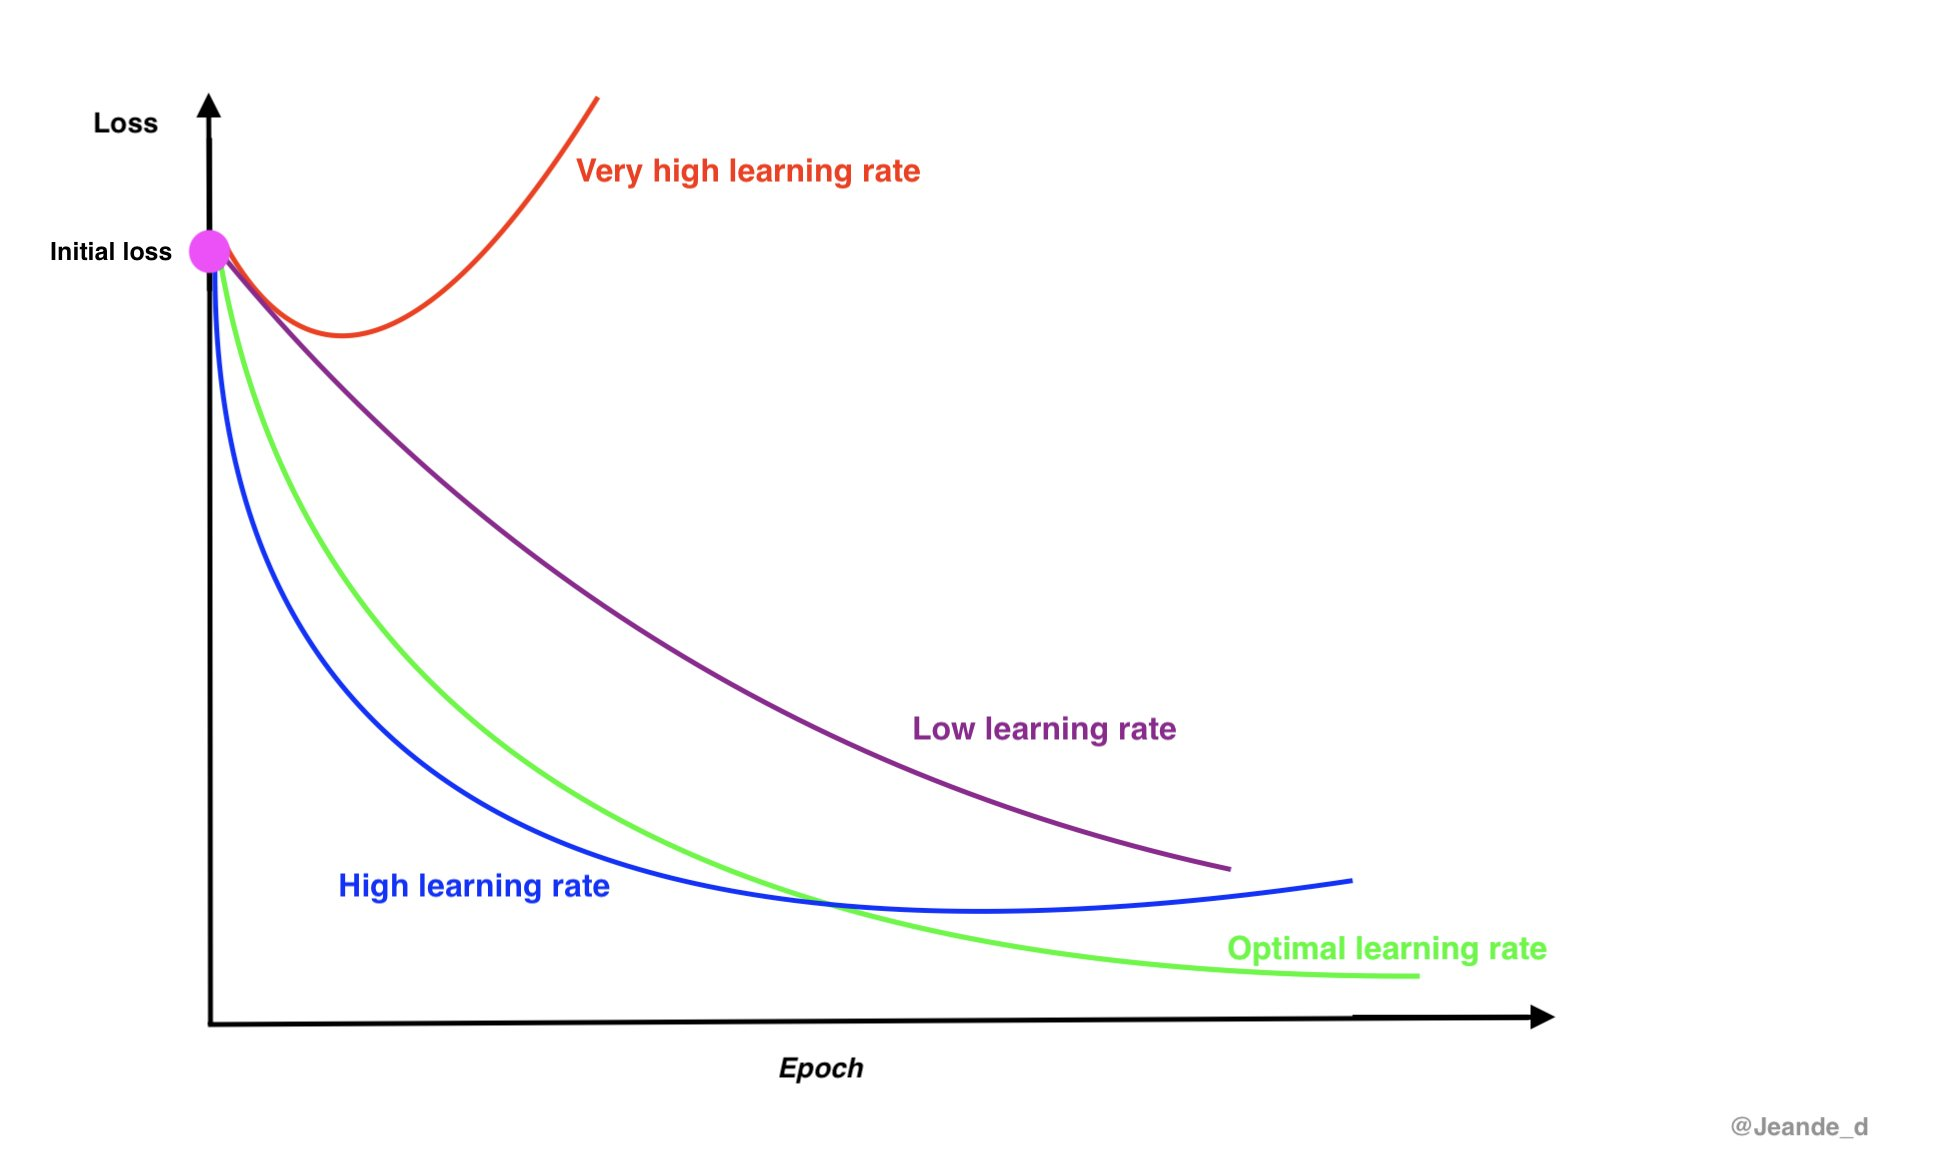
\includegraphics[width=0.5\linewidth]{img/Learning curve and eta.png}
\end{figure}
In a practical approach, it's useful to consider the mean of the gradients over the epoch, in order to have a uniform approach with respect to the number of input data. When using LMS, dividing by $l$ is equivalent to using $\eta/l$ as our learning rate. As a way to improve the choice of learning rate, the following approaches may be considered:

\begin{itemize}
    \item Using \textbf{momentum}: by adding momentum, $\Delta w$ is now calculated as:
    \begin{equation*}
        \Delta w = - \eta \dfrac{\partial E(w)}{\partial w} + \alpha \Delta w_{old} \, ,
    \end{equation*}
    so we introduce a new term that depends on the previous value of $\Delta w$. $\alpha$ is a value between 0 and 1.

    This is called the ``heavy ball method''. It's faster in plateaus, because the same sign of gradient causes the momentum to increase the delta, and also compensates oscillations in the training, allowing us to use a higher value of $\eta$. It's commonly assumed to help with batch mode more, but can also be used with on-line; in this case, $\Delta w_{old}$ is the $\Delta w_{p-1}$ (as in, of the previous example).

    A variant of momentum is the \textbf{Nesterov momentum}, where the gradient is evaluated after the momentum is applied; so we firs calculate $w = w + \alpha \Delta w_{old}$, the we evaluate the gradient on this new $w$. This variant has been shown to improve the rate of convergence for the batch mode, but not for the stochastic mode.
    
    \item Variable learning rate (start high, then decrease):
    using minibatch, the gradient does not reach 0 even when close to a minimum (as exact gradient can do), hence a fixed learning rate should be avoided. We can linearly decay $\eta$ for each step until iteration $\tau$, using $\alpha = step / \tau$:
    \begin{equation*}
        \eta_s = (1-\alpha)\eta_0 + \alpha \eta_{\tau} 
    \end{equation*}
    and then stop for some iteration, from which we can use a fixed small value of $\eta$. Ideally, the final value of $\eta$ should be $\sim 1\%$ of $\eta_0$, so it takes a few hundred steps to reach it.
    
    \item Adaptive learning rates (changed during training and for each $w$): automatically adapt the learning rate during training, avoiding or reducing the fine tuning phase via hyperparameter selection. Some popular ones include AdaGrad, RMSProp, Adam. Can be combined with momentum.
    
    \item Varying in NNs with many layers (higher for deep layers, or higher for units with few input connections).
\end{itemize}

\paragraph{Number of units}

The number of units controls the complexity of the NN. This choice is in general a model selection issue, so it's selected by a cross-validation. Few units typically lead to underfitting, while too many lead to overfitting, but we can have NNs with many units that don't overfit if regularization is used. We can follow two approaches; either a \textbf{constructive}, incremental, one, in which the learning algorithm decides the (small) starting number of units and then adds more as needed, or a \textbf{pruning} one, where we start with a large network and progressively eliminate weights or units.

A common constructive approach is the \textbf{Cascade Correlation (CC)} learning algorithm. It starts with a minimal network, and adds units until the error is low. It learns both the network weights and topology.

\begin{algorithm}
\caption{Cascade Correlation algorithm.}
\begin{algorithmic}[1]
    \State Start with N0, a network with no hidden units, train it and calculate the error.

    \If{N0 does not solve the problem}
        \State Set i = 1.
        \Repeat 
            \State Create a new unit, and add to the network (creating Ni).
            
            \State Train the unit so that the correlation between the output of the unit and residual error of network Ni-1 is maximized.

            \State Freeze the weights of the unit, and retrain all other units.
            
            \State Calculate error of the new network.
            \State Increase i by 1.
        \Until{Error is $\leq$ a given threshold.}
    \EndIf
\end{algorithmic}
\end{algorithm}
Specifically, this algorithm works by interleaving the minimization of the error function with the maximization of the correlation, which is the covariance of the output of the new unit with the residual error. The role of hidden units is to reduce the residual output error.

\subsubsection{Multiple Minima}

Loss in no longer convex. The function may have multiple minima, as well as maxima. The final result depends a lot on the starting weight values. Ideally, we should try a number of random starting configurations (trials), and then take the mean result (as in, the mean of errors) and check the variance in order to evaluate the model. Then, we can either pick the solution that produces the lowest/median validation error, or we can consider the mean of the outputs.

It's worth noting that finding a local minima with too high error that stops training is not a big issue, since we can always check the final training error (and restart if needed). In general, we don't need to find the global minimum, a ``good'' local minima is sufficient. This is because the minimum we find is of $R_{emp}$, not $R$ (which is what we want to approximate). Also, instead of finding a point corresponding to the null gradient, we may want to stop at a point that has sufficiently small gradient.

Another aspects to consider is that the NN builds a variable size hypothesis space, and tends to increase the VC-dim during training. As the VC-dim increases, the $R_{emp}$ decreases towards the global minimum, but we'll likely incur into overfitting, so stopping before we find the minimum might actually produce a better approximation of the target function.

\subsubsection{Stopping Criteria}

The basic stopping criteria is to check the error (mean or max error $ E$), however, we may not always have enough information to set a tolerance threshold for the error. We may want to use an internal criterion: we stop if the improvement of the error (e.g., less than 0.1\%), or the changes to the weights (e.g. norm of gradient $ < \eta$) are negligible.

We must not stop at an arbitrary number of steps; if it's too small, then it may be too early and cause underfitting, while if it is too large, we may incur into overfitting. Also, if we use K-Fold cross validation, the number of ideal steps for each fold may vary: how do we choose it for the final model, trained over all data? We can consider the number of epochs as a hyperparameter, and select its value as the mean across the folds; however, changing the data size at the end, adding all the records of validation and test set, the stop point may be different, leading to underfitting.

\subsubsection{Overfitting and Regularization}

As said before, we typically don't want the global minimizer of $R_{emp}$, since it would be an overfitting solution. The control of complexity requires some form of regularization (as seen for LBE). This can be achieved by introducing a penalty term, or indirectly by early stopping. Another important step is to perform cross-validation on empirical data to find the best trade-off.

In NNs, learning normally starts by setting the weights to small, random values, and the VC-dim is low. As optimization proceeds, hidden units tend to saturate, increasing the number of free parameters, hence increasing the VC-dim. So, how do we choose when to stop this optimization?

\begin{itemize}
    \item \textbf{Early stopping}: using a validation set to determine when to stop. We ideally want to consider multiple epochs to estimate the error. Since the effective number of parameters grows during the course of training, stopping means limiting the complexity.

    \item \textbf{Regularization}: we can use a regularization related to Tikhonov theory, applied to the loss; a penalty term is added, such that the loss will be calculated as:

    \begin{equation*}
        Loss(w) = \sum_p (d_p - o(x_p))^2 + \lambda\|w\|^2
    \end{equation*}
    This is a form of weight decay, since the new values of the weights during gradient descent will be calculated by adding the term $- \lambda w$, which causes it to decrease even when $\Delta w$ is 0. The regularization parameter $\lambda$ is generally a low value, and is selected in the model selection phase.

    \item \textbf{Pruning methods}: will see later.
\end{itemize}

Remember that, when using regularization, the loss is used during model training, while the error (or risk) for the ``data term'' is used during model evaluation, since it only measures how different the output of the hypothesis is from the correct label. A common misconception is that regularization helps convergence stability, but it does not. It only controls the complexity.

Also, early stopping and regularization can be used together. The difference is that early stopping is an \textbf{empirical approach}, that requires a VL set to decide a stopping point, while regularization is a \textbf{principled approach}, and allows the VL curve to follow the TR curve.

Note, also, that the bias $w_0$ is often omitted from the regularizer, since its inclusion causes the results to not be independent from target shift or scaling. If it's included, it has its own regularization term.

\subsubsection{Putting Momentum and Weight Decay Together}

By putting the two together, the $\Delta w$ can be calculated as:

\begin{equation*}
    \Delta w = -\eta \dfrac{\partial Loss(w)}{\partial w_{tu}} + \alpha \Delta w_{old_{tu}} \doteq \eta \delta_t o_u - \lambda w_{tu} + \alpha \Delta w_{old_{tu}}
\end{equation*}
Here, the index $p$ is omitted and we consider the Loss as the sum of Error + Penalty and using $\eta$ only for the Error term. This form, where $\Delta w$ includes $\lambda$, $\eta$ and $\alpha$, is often used by major tools/libraries for NNs. However, we can define a form that keeps the hyperparameters separated, b y writing:

\begin{equation*}
    \Delta w = \eta \delta_t o_u + \alpha \Delta w_{old_{tu}} \, ,
\end{equation*}

\begin{equation*}
    w_{new_{tu}} = w_{tu} + \Delta w_{tu} - \lambda w_{tu} 
\end{equation*}
In this form, eta and alpha are independent.

\subsubsection{Input Scaling/Output Representation}

Preprocessing of the data can have a large effect on the result of training. Data should be normalized via either standardization (each feature is modified so that mean is 0 and standard deviation is 1), or rescaling (the range of values is restricted to [0,1]).

For regression, there's one or more output linear units; for classification, there's either a singular binary output unit, or there's multiple binary units. In the latter case, we can use a sigmoid to choose the threshold to assign the class, a rejection zone, or 1-to-K encoding to choose the ``winner'' class. Often, the symmetric logistic function learns faster. To avoid asymptotic convergence, 0.9 and 0.1 can be used instead of 1 an 0 as a label value (for the logistic function, for the tanh function -0.9 is used instead of -1). In any case, the target range must be in the output range of units. If targets are 0/1, it's common to use the Softmax function:

\begin{equation*}
    o_k(x) = \dfrac{e^{(-net_k)}}{\sum_{j=1}^Ke^{(-net_j)}}
\end{equation*}
We can also use an alternative error/cost function, where we minimize the cross entropy:

\begin{equation*}
   E(w) = - \sum_{i \in TR} \{ d_i \log (out(x_i)) + (1-d_i) \log(1-out(x_i)) \}
\end{equation*}



\section{When To Consider NNs}

\begin{itemize}
    \item The input is high dimensional discrete or real-valued, both for regression and classification tasks;

    \item The dataset possibly contains noise;

    \item The form of the target function is unknown;

    \item Human readability of the output is not critical;

    \item Training time is not critical;
    
    \item The computation of the output itself has to be fast.
\end{itemize}
\chapter{Deep Learning}

\section{Convolutional Neural Networks}

Convolutional Neural Networks are a specialized kind of neural network for processing data with a known, grid-like topology, such as 2D images. The name ``convolutional'' refers to the mathematical operation called \textbf{convolution}, indicated by an asterisk ($*$). This is an operation of two functions of a real valued argument, defined as follows:
\begin{equation*}
    s(t) = (f * g)(t) \stackrel{def}{=} \int_{-\infty}^{\infty} f(\tau)g(t - \tau) d \tau = \int_{-\infty}^{\infty} f(t - \tau)g(\tau) d\tau \,,
\end{equation*}
The idea behind this operator is that we want to calculate the average of $f$ weighted by another function $g$ moved over time (``sliding''), calculated for a certain $t$. In convolutional network terminology, the first argument (here, $f$) is referred to as the \textbf{input}, and the second argument ($g$) as the \textbf{kernel}. The output is called \textbf{feature map}.

This operator can be applied to neural networks as well. Consider a simple network with one hidden layer:
\begin{figure}[h]
    \centering
    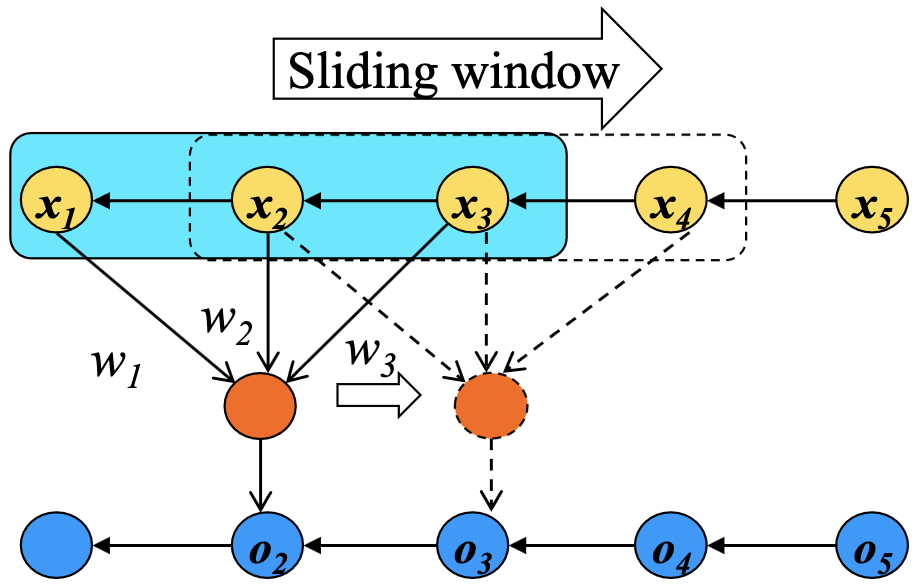
\includegraphics[width=0.45\linewidth]{img/CNN_simple.png}
\end{figure} \\
Here, the output of each node in the hidden layer is calculated as $out_t = \sum_{i=1}^3 w_i x_{t+i-2}$. In other words, the weights assigned to the inputs ``slide'' across the hidden layer. Weights are tuned as usual by learning.

\subsection{2D Convolution}

Discrete convolution can be seen as a multiplication by a matrix, with several entries constrained to be equal to other entries. The convolution over a 2D image $I$ with a kernel $K$ can be expressed as:
\begin{equation*}
    S(i,j) = (I*K)(i,j) = \sum_m \sum_n I(m,n)K(i-m, j-n) \,,
\end{equation*}
or, as expressed by many libraries, as the \textbf{cross-correlation function}:
\begin{equation*}
    S(i,j) = (I*K)(i,j) = \sum_m \sum_n I(i+m,j+n)K(m, n) \,.
\end{equation*}

The example below shows a 2D image with 25 pixels, and a 3x3 kernel (unit local receptive field) with a stride equal to 1 (i.e., the kernel moves across the image 1 pixel at a time; by choosing the stride we choose the size of the feature map). The image also has padding added to its edge.
\begin{figure}[h]
    \centering
    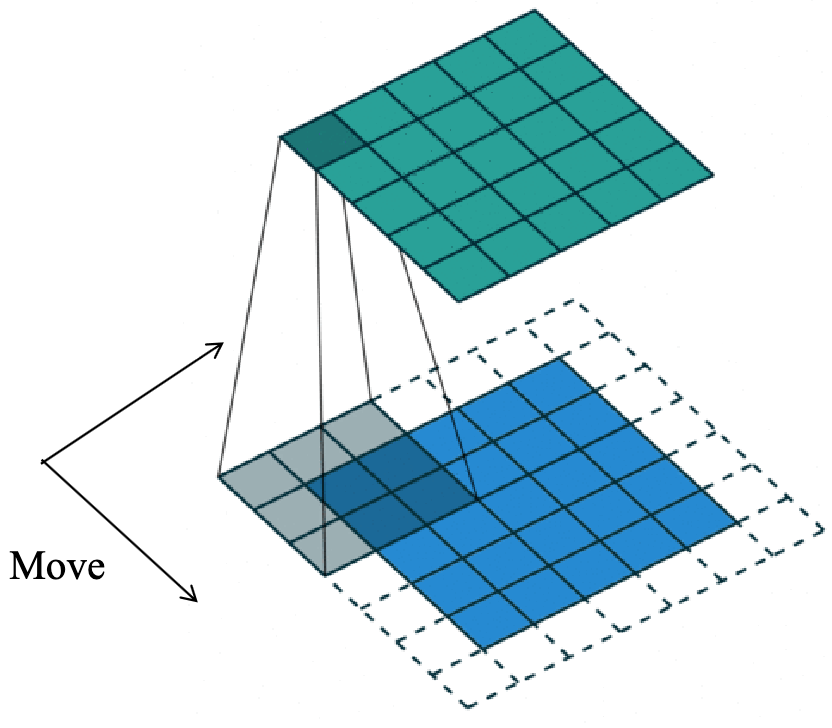
\includegraphics[width=0.6\linewidth]{img/CNN_2D.png} 
\end{figure}

Once the kernel reaches the end of the first ``row'' of pixels, it restarts from the position it started from shifted one pixel below. The full movement of the kernel over the image produces the feature map. The next image better shows the matrix multiplication interpretation of convolution; the image is 4x3 and the kernel is 2x2. The stride is again equal to 1.

\begin{figure}[h]
    \centering
    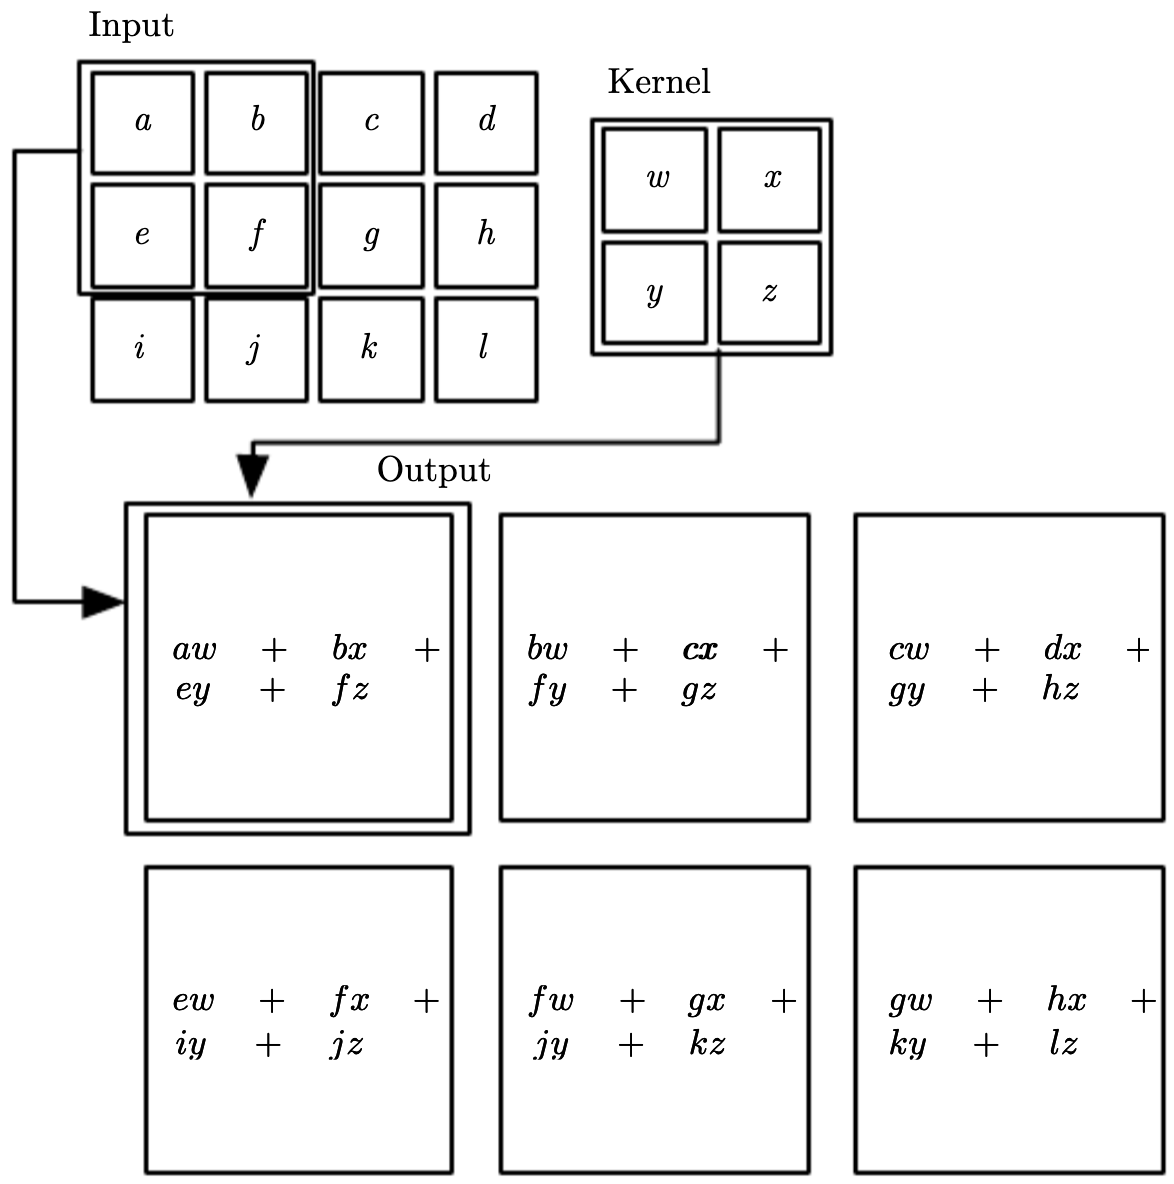
\includegraphics[width=0.5\linewidth]{img/CNN_matrix.png}
\end{figure}
Each unit's weights are a \textbf{filter} trained to detect some specific feature or pattern in the image. Each filter produces the strongest response to a spatially local input pattern, and then the filters obtained by training are applied to the whole (global) image, so that features and patterns can be identified regardless of where they are positioned on the image. \\
The size of the feature map can be reduced via pooling. Some examples of pooling are:
\begin{itemize}
    \item \textbf{Subsampling}, using a stride greater than 1;
    \item \textbf{Average Pooling} (normal or weighted average);
    \item \textbf{Max Pooling} (most common option).
\end{itemize}
This way, instead of producing a value for every single pixel of the original image, we get a smaller set of pixels where each value is obtained by considering the values of neighboring ones (calculating the mean or max value). Pooling also helps to make the representation approximately invariant to small translations of the input, since the mean or max value of a neighborhood of points is unlikely to be affected by a small translation of the pixels in the image.

CNN exploits \textbf{weight sharing}, where the number of connections in the network is kept the same while reducing the number of actual free parameters. The produced sliding window of units is applied over a segment of the input, and reapplied multiple times to produce various layers of feature maps. Training of the weights is usually done via backpropagation. Since these networks tend to be big and deal with large amount of data, many hyperparameters are fixed by experience or by suggestions of experts, since it would be too expensive to run cross-validation.

\section{Deep Learning}

The Deep Learning framework includes many different models, such as:
\begin{itemize}
    \item Deep Neural Networks;
    \item Convolutional Neural Networks;
    \item Deep belief Networks;
    \item Recurrent and Recursive Neural Networks.
\end{itemize}
They differ from ``shallow'' models in that they have a big amount of layers.

The core concept at the base of deep learning is increasing the level of abstraction of the data through the use of several layers; for example, an image can be gradually abstracted on each layer, first as a vector of intensity values per pixel, then a set of edges, then regions of a particular shape, and so on. We've already mentioned this idea with CNNs: the original complicated mapping is broken down into its simple elements, by gradually calculating simpler mapping at each layer. A series of hidden layers extracts increasingly abstract features from a set of example images. Additionally, these abstract features, once learned by the units, can also be combined together to generalize on examples that were never seen during training.

In general, deeper networks are often able to use less units per layer, thus less free parameters as well and less training data required to achieve a good generalization. Still, many layers may be harder to be trained, so there's a need to improve the techniques we know regarding gradient descent, regularization, and data exploitation.

\subsection{Insights}

\subsubsection{Why So Many Layers?}

Imagine a two-layer circuit of logic gates, which can represent any Boolean function. Any Boolean function can indeed be written as a sum of products (i.e., in disjunctive normal form). With logical circuits of depth two, the number of logic gates required to represent most Boolean functions is exponential w.r.t. input size.

An example of such function is the parity function: it returns 1 if there is an odd number of 1s over $N$ binary inputs (i.e., $N$ bits), 0 otherwise. If we were to implement this function with logic gates, assuming $N$ inputs, we would need:
\begin{equation*}
    \dfrac{2^N}{2} + 1 = 2^{N-1} + 1
\end{equation*}
gates, since we have to perform 1 OR and exactly $2^{N-1}$ ANDs.

We can propose an alternative solution with a polynomial number of gates, by increasing the number of layers to $log(N)$. The solution for $N=8$ is shown below (in a simplified view where each XOR corresponds to 2 AND gates and 1 OR gate). In this solution, the number of gates is greatly reduced from $2^7 + 1 = 129$ to only $7 * 3 = 21$.
\begin{figure}[h]
    \centering
    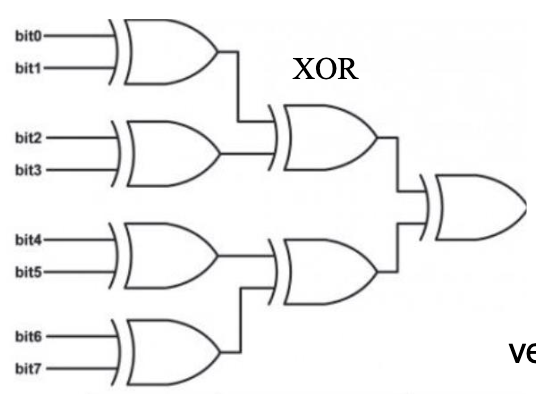
\includegraphics[width=0.5\linewidth]{img/Circuit_deep.png}
\end{figure}

The universal approximation theorem states that even with 1 hidden layer, a NN can approximate any possible function, however it does not specify the number of units needed. For some families of functions a boundary on this number can be found, but as seen in the example above, the bound may be exponential w.r.t. the dimension of the input. Also, there exist families of functions which can be approximated efficiently by a NN with depth greater than some value $d$, but which require a much larger model if depth is restricted to be less or equal than $d$.

This theorem also implies that regardless of what function we are trying to learn, a large MLP is able to represent the function, but there's no guarantee that that the training algorithm will be able to learn that function, either because it can't find the value of the parameters that correspond to the desired function, or because it might choose the wrong function due to overfitting. So another advantage to using multiple layers is ensuring that the learning algorithm can actually properly learn.

The inductive bias is: choosing a deep model encodes the (very general) belief that the function we want to learn should involve composition of several simple functions. If our task actually matches our bias, then the deep shape of the learner is suitable, and those deeper models also perform better than shallow ones. Typically, these tasks are the ones that involve images or language, but for other tasks that deal with different data this deep structure may not be appropriate.

\subsection{Techniques}

When implementing a deep neural network, there's many technical aspects to consider. As already stated before, the deeper the network, the less units are needed for each layer, and therefore there will be less parameters to train, but some layers may be difficult to train. This section will focus on the methods that need improvement and their issued when used with deep NNs.

\textbf{Batch normalization} is a method that normalizes each batch by calculating each individual batch statistics such as mean and variance for each layer. Each matrix (batch x activation of units) is normalized with mean and variance, shifting the values to zero-mean and unit variance. This technique helps to keep the normalization of the input across all layers of the network. It also achieves a faster learning and higher accuracy for Deep Learning.

\textbf{Dropout} is a method that makes bagging more practical for large neural networks. Dropout trains the ensemble consisting of all sub-networks that can be formed by removing non-output units from an underlying base network. In most modern neural networks, we can effectively remove a unit from a network by multiplying its output value by 0. Then, a minibatch-based learning algorithm is used to train one working sub-network at a time. The sub-network is selected at random, with each binary mask to apply to the original network having a different probability set as an hyperparameter (e.g., 0.8 for input units and 0.5 for hidden units). The sub-networks inevitably share weights, since they're obtained from the same base network; this causes the training of the sub-networks to find good settings for the parameters.

Dropout has a regularization effect as well: it avoids to train all units on all training data and reduces unit interactions. It also reduces variance without affecting bias just like bagging does. It even regularizes singular hidden units to be not just good features, but features that can be good in different contexts (different sub-networks). It can be used for any model that uses distributed representation and SGD training.

\section{Recurrent Neural Networks}

Up until now, we considered feedforward neural networks. The input is read from the first layer, then traverses a number of hidden layers, and the prediction is finally produced by the output layer. Recurrent neural networks are a different category of architecture, based on the addition of feedback loops to the network topology. These self loops provide the network with dynamical properties, introducing the ability of holding a memory (state) of past computations of the model.

RNNs have been the reference approach for sequence processing, especially for speech and text recognition, processing, and generation. The type of data handled by these models is structured; it is usually an ordered set of sequences of vectors.

\section{Memory}

The introduction of feedback loops allows the network to hold a memory about past computations. This memory is needed because the output of a certain input depends on previous outputs produced by the same network.
\begin{figure}[h]
    \centering
    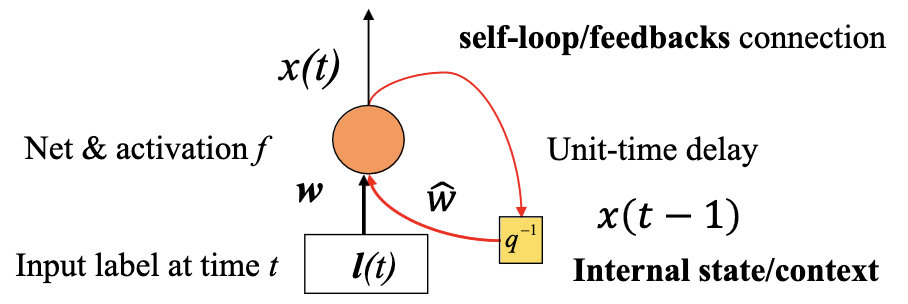
\includegraphics[width=0.5\linewidth]{img/RNN_unit.png}
\end{figure}

The output of the node is calculated for a time $t$ recursively, as:
\begin{equation*}
    x(t) = \begin{cases}
            0 & t = 0 \\
            \tau(i(t), x(t-1)) = f(w^Ti(t) + \hat{w}x(t-1) + \theta) & t \geq 0 \\
    \end{cases}
\end{equation*}
Here, $f$ is the activation function of the unit, $i(t)$ is the input label at time $t$, $\hat{w}$ is the recurrent weight (the one that's coming from a feedback), and $\theta$ is the bias. The internal state summarizes the past information, and changes each time the unit produces a new output. The encoding of the past memory is also adaptive. $\tau$ is the state transition function realized by the NN. $x(t)$ here refers only to one state, but it can also include a set of states.

\section{Properties}

Many RNN architectures are possible, but even a simple one with a few nodes each with its own feedback loop is already incredibly powerful. They are universal approximators of non-linear dynamic systems, and are Turing equivalent (they can simulate any automata).

RNN models are based on the following assumptions:
\begin{itemize}
    \item \textbf{Causality}: a system is causal if the output at time $t_0$ only depends on inputs at time $t<t_0$ (necessary and sufficient for internal state);

    \item \textbf{Stationarity}: time invariance after model training. The state transition function $\tau$ is independent on node $v$ of the sequence.

    \item \textbf{Adaptivity}: transition functions are realized by NN with free parameters, so they are learned from data.
\end{itemize}

RNNs can also be \textbf{unfolded}. Unfolding a RNN means representing it as a graph with a repetitive structure corresponding to a chain of events (so it represents how the same model behaves through time). Unfolding is associated with weight sharing between unfolded layers.
\chapter{Ensemble Learning}

Ensemble methods (also known as classifier combination methods) are used to improve classification accuracy by aggregating the predictions of multiple classifiers. An ensemble method constructs a set of \textbf{base classifiers} trained on the training set (sampled differently depending on the specific technique), and then predicts the output on instances by taking the majority vote.

The key idea that justifies the use of ensemble methods is the so-called \hyperlink{https://en.wikipedia.org/wiki/The_Wisdom_of_Crowds}{\textbf{wisdom of the crowds}}: the collective knowledge of a diverse and independent group of people usually exceeds that of a single individual. According to Surowiecki, there are five elements required to form a wise crowd: diversity of opinion, independence, decentralization, aggregation, and trust. These same elements can be applied to machine learning, where each ``individual'' in the crowd is a model.

To illustrate how a classifier's performance can be improved, consider the following example. \\
We have an ensemble of 25 binary classifiers, each with the same error rate $\varepsilon = 0.35$. The ensemble predicts the class label of a test instance by taking the majority vote on the predictions of the single classifiers. If these classifiers are perfectly identical, then they will all answer the same way on any test input, so the error rate of the ensemble will also be $\varepsilon$.

If instead the base classifiers are independent (their errors are uncorrelated), the ensemble makes a wrong prediction only if more than half of the base classifiers make a mistake; so the error rate of the ensemble is:
\begin{equation*}
    e = \sum_{i=13}^25 \binom{25}{i} \varepsilon^i (1-\varepsilon)^{25 - i} = 0.06
\end{equation*}
which is considerably lower than $\varepsilon$. \\\\
Ensemble classifiers can be constructed in many ways:
\begin{itemize}
    \item By manipulating the training set (bagging, boosting);
    \item By manipulating the input features (random forests);
    \item By manipulating the class labels. (error-correcting output coding).
\end{itemize}

\section{Bagging}

Bagging, which stands for Bootstrap AGGregatING, is a technique that samples with replacement from a data set according to a probability distribution. Given a dataset $X = \{x_1, \dots, x_n \}$, $m$ datasets o size $n$ are sampled from it, such that each record $x_i$ has $\frac{1}{n}$ probability of being extracted. Since replacement is used, the same record may appear multiple times in the same sample, while some records may not appear at all.
\begin{algorithm}
\caption{Bagging algorithm.}
\begin{algorithmic}[1]
    \State Let $k$ be the number of bootstrap samples.

    \For{$i=1$ to $k$}
        \State $D_i$ = Sample of size $N$.
        \State Train a base classifier $C_i$ on $D_i$.
    \EndFor
    \State $C^*(x) = \arg\max_y \sum_i \delta(C_i(x) = y)$
\end{algorithmic}
\end{algorithm} \\
In the above pseudocode, $\delta()$ is a function that returns 1 if its argument is true, 0 else.

Bagging improves generalization error by reducing the variance of the base classifiers. The performance of bagging depends on the stability of the base classifier: if a base classifier is unstable, bagging helps to reduce the errors associated with fluctuations in the training data, and if it is stable, the error of the ensemble will be mainly caused by bias of the base classifier.

\section{Boosting}

Boosting is an iterative procedure used to change the distribution of training examples for base classifiers, increasing weights for instances that are harder to learn. Initially, all instances in the original dataset are assigned a weight equal to $\frac{1}{n}$; a sample is selected (the same way bagging does, with replacement), and a classifier is built on it. All records that are incorrectly classified by this base classifier have their weight increased, while the ones that are correctly classified have theirs decreased. For the next step, another sample is obtained considering the new weights, and used to train a second model. After classifying those instances, their weights are updated, and this goes on until the desired number of boosting rounds is reached.

\subsection{AdaBoost}

In the AdaBoost algorithm, each base classifier $C_i$ is assigned an \textbf{importance}. It depends on the classifier's error rate, defined as:
\begin{equation*}
    \varepsilon_i = \dfrac{1}{l} \sum_{j=1}^l w_j \delta(C_i(x_j) \neq y_i)
\end{equation*}
where $\delta()$ is the same function seen in the bagging pseudocode. The importance is then calculated as:
\begin{equation*}
    \alpha_i = \dfrac{1}{2} \ln \left(\dfrac{1-\varepsilon_i}{\varepsilon_i}\right)
\end{equation*}
When the error is close to 0, the importance is a large positive value, while when the error is close to 1, the importance is a large negative value.
\begin{figure}[h]
    \centering
    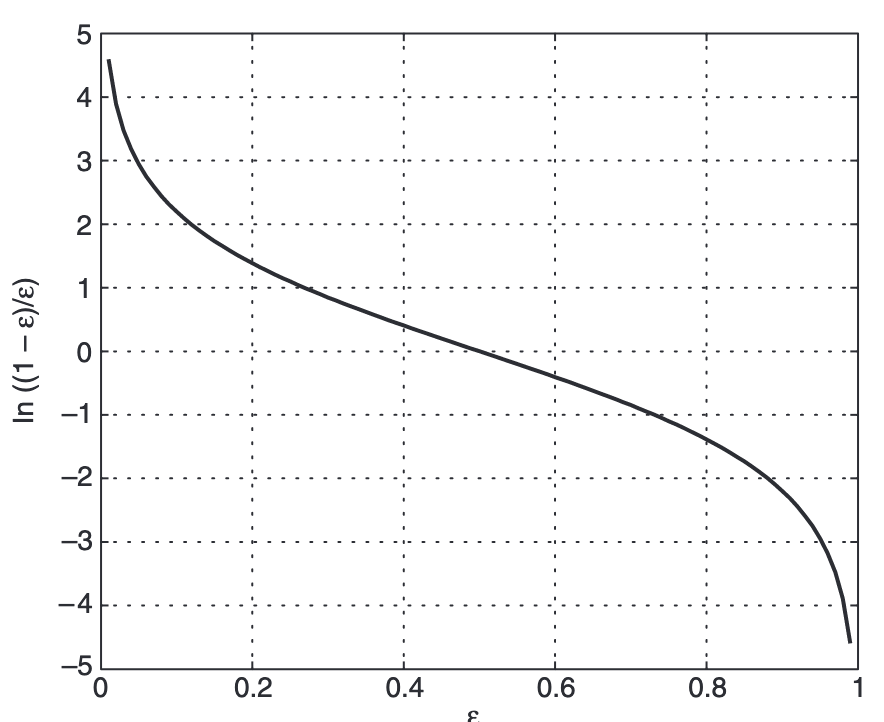
\includegraphics[width=0.4\linewidth]{img/importance_vs_errorrate.png}
    \caption{$\alpha$ as a function of the error rate.}
    \label{fig:importance-errorrate}
\end{figure} \\
The importance is used to update the weights of the training examples, as well. Given an example $x_i$, its corresponding weight at boosting round $j+1$ is:
\begin{equation*}
    w_i^{(j+1)} = \dfrac{w_i^{(j)}}{Z_j} \times \begin{cases}
        e^{-\alpha_j} & C_j(x_i) \neq y_i \\
        e^{\alpha_j} & C_j(x_i) \neq y_i 
    \end{cases}
\end{equation*}
$Z_j$ is the normalization factor, used to ensure that $\sum_i w_i^{(j+1)} = 1$. Using this formula, the weights of examples are increased for those incorrectly classified and decreased for those correctly classified, but the update is influenced by how ``good'' the classifier is. The classification is also influenced by the importance of the classifier:
\begin{equation*}
    C*(x) = \arg\max_y \sum_{j=1}^T \alpha_j \delta(C_j(x) = y)
\end{equation*}
This approach penalizes models with poor accuracy; additionally, if any intermediate boosting round produces an error rate higher than 50\%, the weights of the examples are reverted to their original value $\frac{1}{l}$, and the resampling procedure is repeated.

A default choice of models used by AdaBoost is \textbf{decision stumps}, a decision tree with only the root and two leaf nodes. By themselves, they are very weak learners, but together in an ensemble, they can be very powerful.

\section{Random Forest}

Random forests improve the performances of classifiers by constructing an ensemble of decorrelated decision trees. A key feature of this method is that each base model receives a sample that only selects a subset of the original attributes, usually of dimension $m' \approx \sqrt{m}$, or $m' \approx \log(m)$.

The decision trees used in a random forest are unpruned, as they are allowed to grow to their largest possible size until every leaf is pure. Hence, the base classifiers have lo bias but high variance.

This technique is one of the most accurate learning algorithms available, and is also efficient even on large datasets with thousands of input variables with no need for explicit variable deletion. It also provides an estimate of which variables are most important in classification, and generates an internal unbiased estimate of the generalization error as the forest building progresses.

\appendix
\chapter{Maximum Likelihood Estimation}

Maximum Likelihood Estimation is a method used to determine values for the parameters of a model, such that they maximize the likelihood that the process described by the model produces the observed data. This is done by maximizing a likelihood function, so that the observed data is most probable.

The dataset is modeled as a random sample $x = [x_1, x_2, \dots, x_n]$ of i.i.d. points, taken from an unknown joint probability distribution, expressed in terms of parameters $\theta = [\theta_1, \theta_2, \dots, \theta_k]^T$, so that the distribution falls within the set $\{f(\cdot; \theta) | \theta \in \Theta \}$, where $\Theta$ is the parameter space. Evaluating the joint density at $x$ is
\begin{equation*}
    \mathcal{L}_n(\theta) = \mathcal{L}_n(\theta; x) = f_n(x;\theta) = \prod_{i=1}^n f_n(x_i;\theta)
\end{equation*}
called the likelihood function. The goal is to find the $\theta$ which maximizes it:
\begin{equation*}
    \theta = \arg \max_{\theta \in \Theta} f_n(x;\theta)
\end{equation*}
Since this maximum is found by differentiation, it is often convenient to use the natural logarithm of the likelihood function, called \textbf{log-likelihood}:
\begin{equation*}
    l(\theta;x) = \ln \mathcal{L}_n (\theta;x)
\end{equation*}

Sometimes there's known estimators for the parameters; for example, when assuming a Gaussian distribution, the $\mu$ parameter is estimated as the arithmetic mean of the available observations.
\chapter{Odds and Log Odds}

Given an event with probability $p$, the \textbf{odds} of that even occurring are:
\begin{equation*}
    \textit{odds} = \dfrac{p}{1-p}
\end{equation*}
The \textbf{log-odds} of that event occurring are:
\begin{equation*}
    \ln \left(\dfrac{p}{1-p} \right)
\end{equation*}
An \textbf{odds ratio} is a statistic that quantifies the strength of the association between two events $x$ and $y$, and is calculated as the ratio of the odds of the to events:
\begin{equation*}
    \textit{odds ratio} = \dfrac{\dfrac{p_x}{1-p_x}}{\dfrac{p_y}{1-p_y}}
\end{equation*}
For example, consider the following contingency table:
\begin{center}
\begin{tblr}{
hline{1-2}={3-4}{1pt},
hline{3-5}={1-4}{1pt}, 
vline{3-5}={1-4}{1pt},
vline{1-2}={3-4}{1pt},
colspec = {cccc}}
    & & \SetCell[c=2]{c} Has Cancer & \\
    & & Yes & No \\
    \SetCell[r=2]{c} Has Mutation & Yes & 23 & 117 \\
    & No & 6 & 210 \\
\end{tblr}
\end{center}
We want to know if there is a relationship between the presence of a mutated gene and cancer. The odds ratio is:
\begin{equation*}
    \dfrac{\dfrac{23}{117}}{\dfrac{6}{210}} = \dfrac{0.2}{0.03} = 6.88
\end{equation*}
The result tells us that if someone has a mutated gene, the odds of having cancer are 6.88 higher than for those who do not have a mutation.

\nocite{*}
\bibliographystyle{unsrt}
\clearpage\bibliography{bibliography}

\end{document}
